% BU ECE template for MS thesis and PhD dissertation.
%
%==========================================================================%
% MAIN PREAMBLE 
%==========================================================================%
\documentclass[12pt,letterpaper]{report}          % Single-sided printing for the library
%\documentclass[12pt,twoside]{report} % Double-sided printing
\usepackage[intlimits]{amsmath}
\usepackage{amsfonts,amssymb,amsthm,mathtools}
\usepackage{enumitem}
\DeclareSymbolFontAlphabet{\mathbb}{AMSb}
%\usepackage{natbib}
\usepackage{apalike}
\usepackage{float}
\usepackage[bf]{caption}       
\setcaptionmargin{0.5in}
\usepackage{fancyhdr}
%\usepackage{fancyheadings}
\usepackage{fancybox}
\usepackage{ifthen}
\usepackage{bu_ece_thesis}
\usepackage{url}
\usepackage{lscape,afterpage}
\usepackage{xspace}
\usepackage{epstopdf} 
\usepackage{subfig}

%==========================================================================%
%%% graphicx and pdf creation
\usepackage{graphicx}
\usepackage{appendix}
\usepackage{tikz}
\usetikzlibrary{arrows,calc}
\usepackage{pgfplots}
%\usepackage{psfrag}
%\DeclareGraphicsExtensions{.eps}   % extension for included graphics
%\usepackage{thumbpdf}              % thumbnails for ps2pdf
%\usepackage[ps2pdf,                % hyper-references for ps2pdf
%bookmarks=true,%                   % generate bookmarks ...
%bookmarksnumbered=true,%           % ... with numbers
%hypertexnames=false,%              % needed for correct links to figures !!!
%breaklinks=true,%                  % breaks lines, but links are very small
%linkbordercolor={0 0 1},%          % blue frames around links
%pdfborder={0 0 112.0}]{hyperref}%  % border-width of frames 
%                                   % will be multiplied with 0.009 by ps2pdf
%\hypersetup{
%  pdfauthor   = {Joe Graduate <joe.graduate@bu.edu>},
%  pdftitle    = {dissertation.pdf},
%  pdfsubject  = {doctoral dissertations},
%  pdfkeywords = {mathematics, science, technology},
%  pdfcreator  = {LaTeX with hyperref package},
%  pdfproducer = {dvips + ps2pdf}
%}
\usepackage{cleveref}

\usepackage{thmtools}
\usepackage{thm-restate}
%==========================================================================%
% customized commands can be placed here
\newcommand{\mcX}{\mathcal{X}}
\newcommand{\mcU}{\mathcal{U}}
\newcommand{\mcQ}{\mathcal{Q}}

% Common sets
\newcommand{\Z}{\mathbb{Z}}
\newcommand{\R}{\mathbb{R}}
\newcommand{\N}{\mathbb{N}}


% Environements
\newtheorem{defn}{Definition}
\newtheorem{prop}{Proposition}
\newtheorem{lem}{Lemma}
\newtheorem{theorem}{Theorem}
\newtheorem{assum}{Assumption}

\crefname{lem}{lemma}{lemmas}
\Crefname{lem}{Lemma}{Lemmas}
\crefname{assum}{assumption}{assumptions}
\Crefname{assum}{Assumption}{Assumptions}
%==========================================================================%

%==========================================================================%
% BEGIN
%==========================================================================%
\begin{document}
	
	% The preliminary pages
	% !TeX root = ../thesis.tex
% This file contains all the necessary setup and commands to create
% the preliminary pages according to the buthesis.sty option.

\title{Kink-like Solutions for the FPUT Lattice and the mKdV as a Modulation Equation}
\author{Trevor Norton}

% Type of document prepared for this degree:
%   1 = Master of Science thesis,
%   2 = Doctor of Philisophy dissertation.
%   3 = Master of Science thesis and Doctor of Philisophy dissertation.
\degree=2

\prevdegrees{B.S., Virginia Polytechnic Institute and State University, 2015\\
	M.S., Virginia Polytechnic Institute and State University, 2018}

\department{Department of Mathematics and Statistics}

% Degree year is the year the diploma is expected, and defense year is
% the year the dissertation is written up and defended. Often, these
% will be the same, except for January graduation, when your defense
% will be in the fall of year X, and your graduation will be in
% January of year X+1
\defenseyear{2023}
\degreeyear{2023}

% For each reader, specify appropriate label {First, Second, Third},
% then name, and title. IMPORTANT: The title should be:
%   "Professor of Electrical and Computer Engineering",
% or similar, but it MUST NOT be:
%   Professor, Department of Electrical and Computer Engineering"
% or you will be asked to reprint and get new signatures.
% Warning: If you have more than five readers you are out of luck,
% because it will overflow to a new page. You may try to put part of
% the title in with the name.
\reader{First}{C. Eugene Wayne, PhD}{Professor of Mathematics}
\reader{Second}{Tasso Kaper, PhD}{Professor of Mathematics}
\reader{Third}{Margaret Beck, PhD}{Professor of Mathematics}
\reader{Fourth}{Ryan Goh, PhD}{Assistant Professor of Mathematics}

% The Major Professor is the same as the first reader, but must be
% specified again for the abstract page. Up to 4 Major Professors
% (advisors) can be defined. 
\numadvisors=1
\majorprof{C. Eugene Wayne, PhD}{{Professor of Mathematics}}
%\majorprofb{First M. Last, PhD}{{Professor of Astronomy}}
%\majorprofc{First M. Last, PhD}{{Professor of Biomedical Engineering}}

%%%%%%%%%%%%%%%%%%%%%%%%%%%%%%%%%%%%%%%%%%%%%%%%%%%%%%%%%%%%%%%%  

%                       PRELIMINARY PAGES
% According to the BU guide the preliminary pages consist of:
% title, copyright (optional), approval,  acknowledgments (opt.),
% abstract, preface (opt.), Table of contents, List of tables (if
% any), List of illustrations (if any). The \tableofcontents,
% \listoffigures, and \listoftables commands can be used in the
% appropriate places. For other things like preface, do it manually
% with something like \newpage\section*{Preface}.

% This is an additional page to print a boxed-in title, author name and
% degree statement so that they are visible through the opening in BU
% covers used for reports. This makes a nicely bound copy. Uncomment only
% if you are printing a hardcopy for such covers. Leave commented out
% when producing PDF for library submission.
%\buecethesistitleboxpage

% Make the titlepage based on the above information.  If you need
% something special and can't use the standard form, you can specify
% the exact text of the titlepage yourself.  Put it in a titlepage
% environment and leave blank lines where you want vertical space.
% The spaces will be adjusted to fill the entire page.
\maketitle
\cleardoublepage

% The copyright page is blank except for the notice at the bottom. You
% must provide your name in capitals.
\copyrightpage
\cleardoublepage

% Now include the approval page based on the readers information
\approvalpage
\cleardoublepage

% Here goes your favorite quote. This page is optional.
%\newpage
%\thispagestyle{empty}
%\phantom{.}
\vspace{4in}

\begin{singlespace}
\begin{quote}
  \textit{Facilis descensus Averni;}\\
  \textit{Noctes atque dies patet atri janua Ditis;}\\*
  \textit{Sed revocare gradum, superasque evadere ad auras,}\\
  \textit{Hoc opus, hic labor est.}\hfill{Virgil (from Don's thesis!)}
\end{quote}
\end{singlespace}

% \vspace{0.7in}
%
% \noindent
% [The descent to Avernus is easy; the gate of Pluto stands open night
% and day; but to retrace one's steps and return to the upper air, that
% is the toil, that the difficulty.]

%\cleardoublepage

% The acknowledgment page should go here. Use something like
% \newpage\section*{Acknowledgments} followed by your text.
\newpage
\section*{\centerline{Acknowledgments}}
% !TeX root = ../thesis.tex

I would like to thank my advisor, Gene, for all his help with this thesis. He originally suggested the topic of research, and since then he has been giving guidance and feedback on my work. This thesis would not have been possible without his help, and I greatly appreciated having him as an advisor.

%Thank the committee 

%Thank Julio and Mark

%Thank my parents

%Thank Stuart

This research was supported in part by the US National Science Foundation through grant DMS-1813384 whose assistance is gratefully acknowledged.


%\vskip 1in

%\noindent
%Janusz Konrad\\
%Professor\\
%ECE Department
\cleardoublepage

% The abstractpage environment sets up everything on the page except
% the text itself.  The title and other header material are put at the
% top of the page, and the supervisors are listed at the bottom.  A
% new page is begun both before and after.  Of course, an abstract may
% be more than one page itself.  If you need more control over the
% format of the page, you can use the abstract environment, which puts
% the word "Abstract" at the beginning and single spaces its text.

\begin{abstractpage}
% !TeX root = ../thesis.tex
% ABSTRACT

[This is where the text for the abstract will go]

\end{abstractpage}
\cleardoublepage

% Now you can include a preface. Again, use something like
% \newpage\section*{Preface} followed by your text

% Table of contents comes after preface
\tableofcontents
\cleardoublepage

% If you do not have tables, comment out the following lines
%\newpage
%\listoftables
%\cleardoublepage

% If you have figures, uncomment the following line
%\newpage
%\listoffigures
%\cleardoublepage

% List of Abbrevs is NOT optional (Martha Wellman likes all abbrevs listed)
\chapter*{List of Abbreviations}
\begin{center}
  \begin{tabular}{lll}
    \hspace*{2em} & \hspace*{1in} & \hspace*{4.5in} \\
    FPUT  & \dotfill & Fermi-Pasta-Ulam-Tsingou \\
    KdV & \dotfill & Korteweg-de Vries \\
    mKdV  & \dotfill & modified Korteweg-de Vries\\
  \end{tabular}
\end{center}
\cleardoublepage

% END OF THE PRELIMINARY PAGES

\newpage
\endofprelim
        
	\cleardoublepage
	
	% -------------------------------------
	% CHAPTER ?: BACKGROUND MATERIAL
	% -------------------------------------
	% !TeX root = ../thesis.tex
\chapter{Background Material}
\section{Fenichel Theory}\label{sec:fenichel_theory}
\cite{wiggins1994normally}

\begin{equation}\label{generic_ode}
	\dot x = f(x), \quad x \in \R^n
\end{equation}

\begin{defn}
	Let \(\overline M = M \cup \partial M\) be a compact, connected \(C^r\) manifold with boundary contained in \(\R^n\). Then \(\overline M\) is said to be \emph{overflowing invariant} under \cref{generic_ode} if for every \(p \in \overline M\), \(\phi_t(p) \in \overline M\) for all \(t\leq 0\) and the vector field \cref{generic_ode} is pointing strictly outward on \(\partial M\).
\end{defn}

%Wiggins Thm. 4.5.1 originally Fenichel 1971
\begin{theorem}\label{unstable-manifold-fenichel}
	Suppose \(\dot x = f(x)\) is a \(C^r\) vector field on \(\R^n\), \(r\geq 1\). Let \(\overline M = M \cup \partial M\) be a \(C^r\), compact connected manifold with boundary overflowing invariant under the vector field \(f(x)\). Suppose \(\nu^s(p) < 1\), \(\lambda^u(p) < 1\), and \(\sigma^s(p) < \frac 1 r\) for all \(p\in M\). Then there exists a \(C^r\) overflowing invariant manifold \(W^u(\overline M)\) containing \(\overline M\) and tangent to \(h_u(N'^u_\epsilon )\) along \(\overline M\) with trajectories in \(W^u(\overline M)\) approaching \(\overline M\) as \(t\to -\infty\).
\end{theorem}

%Wiggins Thm 5.6.1
\begin{theorem}\label{foliation-of-unstable-manifold}
	Suppose \(\dot x = f(x) \) is a \(C^r\) vector field on \(\R^n\), \(r\geq 1\). Let \(\overline M = M \cup \partial M\) be a \(C^r\) compact connected manifold with boundary, overflowing invariant under the vector field \(f(x)\). Suppose \(\lambda^u(p)< 1\), \(\sigma^{cu}(p) < 1\), and \(\sigma^{su}(p) < 1\) for every \(p \in \overline M_1\). Then there exists a \(n-(s+u)\)-parameter family \(\mcF^u = \cup_{p\in M} f^u(p)\) of \(u\)-dimensional surfaces \(f^u(p)\) (with boundary) such that the following hold:
	\begin{enumerate}
		\item \(\mcF^u\) is a negatively invariant family, i.e., \(\phi_{-t} (f^u(p)) = f^u(\phi_{-t}(p))\) for any \(t\geq 0\) and \(p\in M\).
		\item The \(u\)-dimensional surfaces \(f^u(p)\) are \(C^r\).
		\item \(f^u(p)\) is tangent to \(h_u(N'^u_p)\) at \(p\).
		\item There exists \(C_u,\lambda_u > 0\) such that if \(q\in f^u(p)\), then \[| \phi_{-t}(q) - \phi_{-t}(p) | < C_u e^{-\lambda_u t}\] for any \(t\geq 0\).
		\item Suppose \(q\in f^u(p)\) and \(q'\in f^u(p')\). Then \[\frac{|\phi_{-t}(q) - \phi_{-t}(p) |}{| \phi_{-t}('q) - \phi_{-t}(p) |} \to 0 \quad \text{as } t\to\infty\] unless \(p = p'\).
		\item \(f^u(p) \cap f^u(p') = \emptyset \), unless \(p=p'\).
		\item If the hypotheses of the unstable manifold theorem hold, i.e., if additionally \(\nu^s(p) < 1\) and \(\sigma^s(p) < \frac 1 r\) for every \(p \in \overline M_1\), then the \(u\)-dimensional surfaces \(f^u(p)\) are \(C^r\) with respect to the basepoint \(p\).
		\item \(\mcF^u = W_{\mathrm{loc}}^u(M)\).
	\end{enumerate}
\end{theorem}

	\cleardoublepage
	
	% -------------------------------------
	% CHAPTER ?: EXISTENCE OF KINK-LIKE TRAVELLING WAVE SOLUTIONS
	% -------------------------------------
	% !TeX root = ../thesis.tex
\chapter{Existence of Kink-Like Traveling Wave Solutions}
\label{chp:existence}
\pagestyle{myheadings}

\section{Introduction}

The goal of this chapter is to show the existence of the traveling wave solution for the FPUT lattice and describe its profile. From formal calculations and the numerical experiments carried out in \cite{pace2019beta}, it seems that the traveling wave solution has a profile given by the kink solution to the defocusing mKdV, \cref{intro-defocusing-mkdv}; that is, for \(\varphi_1(\cdot) = \frac 1 {\sqrt 2} \tanh(\cdot/\sqrt 2)\) we expect to have a traveling wave solution \(u\) such that 
\begin{equation}\label{formal-approximation}
	u_n(t) = \epsilon \varphi_1(\epsilon(n - ct)) +\mcO(\epsilon^3)
\end{equation}
when \(c\) is slightly smaller than \(V''(0) = 1\).

One would expect that methods used to find the solitary wave solution for the FPUT can also be applied to this case. Notably it was shown in \cite{friesecke1999solitary} that there exists a solitary wave solution whose profile is described by the KdV soliton using a fixed-point argument. The argument relies on creating a map from \(H^1(\R)\) to itself using Fourier multipliers such that the fixed point of the map is the profile of the solitary wave. However, this argument does not seem to extend to our case since the function \(\varphi_1\) is not in a Sobolev space and its Fourier transform is defined only in a distributional sense. Due to this problem, we neglect the functional approach and focus on techniques from bifurcation theory. 

One common technique for constructing traveling wave solutions to PDEs is by using the center manifold theorem. For PDEs of one spatial and one temporal variable, the strategy is to assume that the solution is a traveling wave (i.e.\ of the form \(f(x-ct)\)) to eliminate the derivative with respect to \(t\) and reduce the problem to an ODE with respect to the spatial variable \(x\). Finding bounded solutions of this ODE then results in traveling wave solutions of the PDE. The center manifold is an important tool for finding these solutions since (1) it is typically finite-dimensional, (2) can be approximated by Taylor series up to arbitrary order, and (3) contains all bounded solutions. If a linear operator has an eigenvalue pass through the line \(\{\lambda\in\mathbb C: \Re \lambda = 0\}\) as a parameter \(\mu\) varies, then one can have a center manifold containing small bounded solutions parameterized by \(\mu\). Similar techniques can be used to find center manifold for more general semi-dynamical systems defined on Banach spaces \cite{vanderbauwhede1992center}. Such a construction was carried out in \cite{iooss2000travelling} for an abstract ODE representing an advance delay differential equation. The existence of several traveling wave solutions on the FPUT lattice were proved. The bifurcation parameter in this paper was given in part by the wave speed. In fact, \cite[Thm.\ 5]{iooss2000travelling} shows the existence of a heteroclinic orbit on the center manifold when \(c\) is slightly smaller than \(1\). This heteroclinic orbit corresponds to the kink-like solution of the FPUT we are interested in. But no description of its wave profile was given, so obtaining an estimate of the form in \cref{formal-approximation} is still an open problem.


Our argument for getting such an estimate will proceed as follows. We first follow the procedure in \cite{iooss2000travelling}
to construct the center manifold parameterized by \(\epsilon\), making sure to explicitly compute the dynamics on the center manifold. Making a suitable change of variables, we look for small-amplitude, long-wavelength solutions for the FPUT on the center manifold and show that formally setting \(\epsilon = 0\) gives a solution related to the kink solution \(\varphi_1\). Next we apply results from Fenichel theory to show that this solution persists for \(\epsilon> 0\). Lastly we convert our results back to the original formulation of the FPUT lattice and prove an estimate of the form \cref{formal-approximation}.


%Main result here?

\section{Construction of Center Manifold}
%Change of coordinates to get into the form of an abstract ODE.
We follow the construction of the center manifold carried out in \cite{iooss2000travelling}. Recall that the equations for the FPUT lattice are given by
\begin{equation*}
	\ddot x_n = V'(x_{n+1} - x_n) - V'(x_n - x_{n-1}), \quad n \in \Z. \tag{\ref{fput-lattice-odes}}
\end{equation*}
We assume that \(V(x) = \frac 12 x^2 - \frac 1 {24} x^4 + \mcO(x^5)\) near \(x=0\). This choice of potential is chosen so that \(V''(0) = 1\) and \(V^{(4)}(0) = -1\); if we have a potential where \(V(0) = V'''(0)=0\), \(V''(0) > 0\) and \(V^{(4)}(0)< 0\), we can rescale to get the potential above. We make the ansatz that 
\begin{equation}
	x_n(\tilde t) = x(n-c\tilde t),
\end{equation}
where the \(x(t)\) on the right is a function from \(\R\) to \(\R\). Hence \(x(t)\) must satisfy the advance-delay differential equation
\begin{equation}\label{advance-delay-equation}
	\ddot x (t) = \mu \Big(V'(x(t+1) - x(t)) - V(x(t) - x(t-1)) \Big)
\end{equation}
where \(\mu = c^{-2}\). For delay differential equations like the one above, we are inherently working with an infinite-dimensional problem; the dynamics of \(x(t)\) are determined by its value on an interval of \(t\). Instead of working directly with \cref{advance-delay-equation}, we rewrite the equation as a first-order differential equation in a Banach space. \Cref{advance-delay-equation} cannot be written as a differential equation in a finite-dimensional phase space, and so we use a Banach space to represent a ``slice'' of the function on the interval \([t-1,t+1]\) for \(t\in\R\). We introduce a new variable \(v\in[-1,1]\) and functions \(X(t,v) = x(t+v)\). We use the notation \(\xi(t) = \dot x(t)\), \(\delta^1X(t,v) = X(t,1)\), and \(\delta^{-1} X(t,v) = X(t,-1)\). Then letting \(U(t) = (x(t), \xi(t), X(t,v))^T\) represent our solution, \cref{advance-delay-equation} can be written as follows:
\begin{equation}\label{first-order-abstract-ode}
	\partial_t U = L_\mu U + M_\mu (U)
\end{equation}
where \(L_\mu\) is the linear operator %Explain \partial_\nu. Corresponds to shift, but how do we get unique solutions?
\begin{equation}
	L_\mu = \begin{pmatrix}
		0 & 1 & 0\\
		-2\mu & 0 & \mu(\delta^1 + \delta^{-1}) \\
		0 & 0 & \partial_v
	\end{pmatrix}
\end{equation}
and 
\begin{equation}
	M_\mu(U) = \mu (0, g(\delta^1X -x) - g(x- \delta^{-1} X), 0)^T
\end{equation}
where we define \(g(x)= V'(x) - x\). Note the second component of \cref{first-order-abstract-ode} corresponds with the advance-delay equation. The third component corresponds to the functional part  \(X(t,\nu)\) and gives \(\partial_t X = \partial_\nu X\), so that the solution is given by a translation . We will also require that \(X(t,0) = x(t)\), so that \(X(t,v) = x(t+v)\) and solutions of \cref{first-order-abstract-ode} correspond with solutions of \cref{advance-delay-equation}. We introduce the following Banach spaces for \(U\):
\begin{equation}
	\begin{aligned}
		\bbH &= \R^2 \times C[-1,1] \\
		\bbD &= \{(x, \xi, X) \in \R^2 \times C^1[-1,1] \mid X(0) = x\}
	\end{aligned}
\end{equation}
where the spaces have the usual maximum norms. The operator \(L_\mu\) is continuous from \(\bbD\) to \(\bbH\). Assuming that \(g\in C^4(I)\) where \(I\) is an open neighborhood around \(0\), we have \(M_\mu \in C^4(\bbD,\bbD)\).

The system above has a reversibility symmetry \(S\) given by 
\begin{equation}
	S(x, \xi, X)^T = (-x, \xi, -X \circ s)^T
\end{equation}
where \(X\circ s (v) = X(-v)\). That is, \cref{first-order-abstract-ode} is reversible and if \(U(t)\) is a solution then so is \((S\circ U)(-t)\). Additionally, if \(V'(x)\) is odd, then \cref{first-order-abstract-ode} is also odd; this means that if \(U(t)\) is a solution then so is \(-U(t)\).

Note that \cref{first-order-abstract-ode} does not have all solutions in \(\mathbb D\) and so some may not correspond with the requirement that \(X(t,0) = x(t)\). However, we can show that there is a center manifold which contains global solutions and lies in \(\bbD\), and so we will be able to extract the traveling wave solutions that we are interested in.

%The linear operator has a quadruple zero eigenvalue when mu = 1. 
%Write out the eigenvectors and their corresponding projection operators
As shown in \cite[Lem.\ 1]{iooss2000travelling}, when \(\mu = \mu_0:= 1\) (i.e.\ when \(c = \sqrt{V''(0)} = 1\)) the linear operator \(L_{\mu_0}\) has a quadruple zero eigenvalue with the rest of the spectrum bounded uniformly away from the imaginary axis. This allows for the construction of a four-dimensional center manifold. This construction is not carried out explicitly in \cite{iooss2000travelling}, but it follows similarly to the calculations carried out in \cite{iooss2000travelling2} which relies on results in \cite{vanderbauwhede1992center}.

The four-dimensional eigenspace for \(\lambda = 0\) is spanned by the following generalized eigenfunctions:
\begin{equation}
	\begin{aligned}
		&\zeta_0 = (1,0,1)^T  & &\zeta_1 = (0,1,v)^T \\
		&\zeta_2 = (0, 0, \frac 12 v^2)^T & &\zeta_3 = (0,0,\frac 1 6 v^3)^T
	\end{aligned}
\end{equation}
which satisfy
\begin{equation}
	\begin{aligned}
		L_{\mu_0} \zeta_0 &= 0 \\
		L_{\mu_0} \zeta_1 &= \zeta_0 \\
		L_{\mu_0} \zeta_2 &= \zeta_1 \\
		L_{\mu_0} \zeta_3 &= \zeta_2.
	\end{aligned}
\end{equation}
The spectral projection onto the eigenspace can be found using the Laurent expansion in \(\mcL(\bbH)\) near \(\lambda = 0\)
\begin{equation}
	(\lambda \mathrm I - L_{\mu_0} )^{-1} = \frac{D^3}{\lambda^4} + \frac{D^2}{\lambda^2} + \frac{D}{\lambda^2} + \frac P \lambda - \tilde L _{\mu_0} ^{-1} + \lambda \tilde L_{\mu_0} ^{-1} - \cdots
\end{equation}
where \(P\) is the spectral projection onto the \(\lambda = 0\) eigenspace, \(D = L_{\mu_0} P\), and \(\tilde L _{\mu_0} ^{-1}\) is the pseudo-inverse of \(L_{\mu_0}\) on the subspace \((\mathrm I - P)\bbH\) (see \cite{kato2013perturbation}). The spectral projection satisfies %Is there a better citation for this?
\begin{equation}
\begin{aligned}
	PW &= ((PW)_x, (PW)_\xi, (PW)_X)^T \\
	&= (PW)_x \zeta_0 + (DW)_x\zeta_1 + (D^2W)_x\zeta_2 + (D^3W)_x \zeta_3
\end{aligned}
\end{equation}
The projection operator has an explicit form given by 
\begin{equation}
	P = \oint_\gamma (\lambda I - L_\mu)^{-1} \, d\lambda
\end{equation}
where \(\gamma\) is a curve going around \(\lambda = 0\) counter-clockwise and not intersecting the spectrum of \(L_\mu\). The projection can be computed by first finding the resolvent \((\lambda \mathrm I - L_\mu)^{-1}\) and then using the residue theorem to compute the integral. 

The resolvent operator is straightforward to find. For \(F=(f_0,f_1,F_2)^T\in\bbH\), we want to find \(U = (x,\xi, X)^T\in \bbD\) such that
\begin{equation}
	(\lambda I a- L_\mu) U = F.
\end{equation}
The above is a differentil equation with coupled algebraic equations. The operator on the left-hand side is invertible when \(N(\lambda ;\mu) \neq 0\), where 
\begin{equation}
	N(\lambda;\mu) = - \lambda^2 + 2\mu(\cosh \lambda - 1).
\end{equation}
Solving for \(U\) gives
\begin{align}
	x &= -[N(\lambda;\mu)]^{-1}(\lambda f_0 + f_1 + \mu\tilde f_\lambda) \\
	\xi &= -[N(\lambda;\mu)]^{-1} \Big( [\lambda^2 + N(\lambda;\mu)]f_0 + \lambda f_1 + \mu\lambda \tilde f_\lambda \Big) \\
	X(v) &= e^{\lambda v}x - \int_0^v e^{\lambda(v-s)} F_2(s)\, ds
\end{align}
with 
\begin{equation}
	\tilde f_\lambda = \int_0^1 [-e^{\lambda(1-s)} F_2(s) + e^{-\lambda (1-s)} F_2(-s)]\, ds.
\end{equation}
The projection can be computed by using the residue theorem. For instance, note that 
\begin{equation}
	(PF)_x = \mathrm{Res}(((\lambda  I - L_{\mu_0})^{-1} F)_x, 0) = \mathrm{Res}(-[N(\lambda;\mu_0)]^{-1}(\lambda f_0 + f_1 + \mu_0\tilde f_\lambda), 0).
\end{equation}
For fixed \(F\in\bbH\), the last term can be found by finding the residue of a meromorphic function in \(\bbC\). For example, we can compute that the Laurent series of \(-[N(\lambda,\mu_0)]^{-1}\) is given by
\begin{equation}
	-[N(\lambda;\mu_0)]^{-1} = \frac  1 {\lambda^2 - 2(\cosh\lambda - 1)} = \frac{-12}{\lambda^4} + \frac{2}{5\lambda^2} - \frac{13}{2100} + \cdots.
\end{equation}
Similarly, we have the power series representation
\begin{equation}
	\begin{aligned}
		\int_0^1[-e^{\lambda(1-s) } F_2(s) + e^{-\lambda (1-s)} F_2(-s)]\, ds = &- \int_0^1[F_2(s) - F_2(-s)] \, ds \\
		&\quad - \lambda  \int_0^1 (1-s)[F_2(s) + F_2(-s)]\, ds \\
		&\quad - \frac{\lambda^2}{2} \int_0^1 (1-s)^2[F_2(s) - F_2(-s)]\, ds \\
		&\quad - \frac{\lambda^3}{6} \int_0^1 (1-s)^3[F_2(s) + F_2(-s)]\, ds \\
		&\quad + \cdots
	\end{aligned}
\end{equation}
Thus taking a convolution of the Laurent series and finding the \(-1\)st coefficient yields
\begin{equation}
\begin{aligned}
	&\mathrm{Res}(-[N(\lambda;\mu_0)]^{-1}(\lambda f_0 + f_1 + \mu_0\tilde f_\lambda), 0)&\\
	&\quad= \frac 2 5 f_0 - \frac 2 5 \int_0^1 (1-s)[F_2(s) + F_2(-s)]\, ds + 2 \int_0^1 (1-s)^3[F_2(s) + F_2(-s)]\, ds \\
	&\quad =  \frac 2 5 \Bigg(  f_0 - \int_0^1[(1-s) - 5(1-s)^3][F_2(s) + F_2(-s)]\, ds \Bigg) .
\end{aligned}
\end{equation}
Proceeding in this way, we can get  
\begin{align}
	(PF)_x &= \frac 2 5 \Bigg(  f_0 - \int_0^1[(1-s) - 5(1-s)^3][F_2(s) + F_2(-s)]\, ds \Bigg) \\
	(DF)_x &= (PF)_\xi = \frac 2 5 \Bigg(  f_1 - \int_0^1[1 - 15(1-s)^2][F_2(s) - F_2(-s)]\, ds \Bigg) \\
	(D^2F)_x &= (DF)_\xi = -12 \Bigg( f_0 - \int_0^1(1-s)) [F_2(s) + F_2(-s)]\, ds \Bigg) \\
	(D^3F)_x &= (D^2 F)_\xi = -12 \Bigg(f_1 - \int_0^1 [F_2(s) - F_2(-s)]\, ds \Bigg).
\end{align}
We denote by \(\zeta_j^*\) the linear continuous forms on \(\bbH\) given for any \(F\in\bbH\) by
\begin{equation}
	\begin{aligned}
		\zeta_0^*(F)&= (PF)_x \\
		\zeta_1^*(F) &= (DF)_x  = \zeta_0^*(L_{\mu_0} F) \\
		\zeta_2^*(F) &= (D^2F)_x  \\
		\zeta_3^*(F) &= (D^3F)_x 
	\end{aligned}
\end{equation}
and we have that
\begin{equation}
	\zeta_k^*(\zeta_j) = \delta_{kj} \quad k,j = 0, 1, 2, 3
\end{equation}
where \(\delta_{kj}\) is the Kronecker delta.

%Go through the invariance argument to reduce to three eigenvectors (the invariance is a shift invariance on the original lattice).
At this point we could start to compute the four-dimensional center manifold parameterized by \(\mu\), but we can do a further simplification. Note that \cref{first-order-abstract-ode} is invariant under 
\begin{equation}
	U \mapsto U + q \zeta_0, \quad \forall q \in \R
\end{equation}
which corresponds to the shift invariance of \cref{advance-delay-equation}. This invariance allows us to reduce the center manifold to a three-dimensional manifold. We first decompose \(U \in \bbH\) as follows:
\begin{equation}
	U = W + q \zeta_0, \quad \zeta_0^*(W) = 0.
\end{equation}
Denote by \(\bbH_1\) the codimension-one subspace of \(\bbH\) where \(\zeta_0^*(W) = 0\), and similarly define \(\bbD_1\). Then the system in \cref{first-order-abstract-ode} becomes
\begin{align}
	\frac{dq}{dt} &= \zeta_0^*(L_{\mu} W) = \zeta_0^*(L_{\mu_0} W) = \zeta_1^*(W) \label{ode-for-q} \\
	\frac{d W}{dt} &= \widehat{L}_\mu W + M_\mu(W) \label{reduced-first-order-system}
\end{align}
where \(\widehat{L}_\mu W = L_\mu W - \zeta_1^*(W)\zeta_0\). The operator \(\widehat L_{\mu_0}\) acting on \(\bbH_1\) has the same spectrum as \(L_{\mu_0}\) except that \(0\) is now a triple eigenvalue instead of a quadruple eigenvalue. One can check that
\begin{equation}\label{reduced-eigenfunction}
	\widehat{L}_{\mu_0} \zeta_1 = 0, \quad \widehat{L}_{\mu_0}\zeta_2 = \zeta_1, \quad \widehat{L}_{\mu_0}\zeta_3 = \zeta_2, \quad \zeta_3^*(\widehat{L}_{\mu_0}W) = 0.
\end{equation}

% State the center manifold theorem at this point. Should discuss regularity of Phi and that it is in the null space of the spectral projection operators.
Hence we have a three-dimensional center manifold on which solutions are given by
\begin{equation}\label{W-center-manifold}
	W = A \zeta_1 + B\zeta_2 + C\zeta_3 +\Phi_\mu(A,B,C).
\end{equation}
Here \(\Phi_\mu\) takes values in \(\bbD_1\). Note that this implies solutions on the center manifold correspond with solutions of \cref{advance-delay-equation}, as desired. We also have that (1) \(\Phi_\mu\) has the same regularity as \(V'\), (2) it satisfies \(\zeta_k^*(\Phi_\mu) = 0\) for \(k=1,2,3\),  and (3) it is at least quadratic in its arguments.

The symmetries noted before in \cref{first-order-abstract-ode} are preserved in the center manifold \cite{vanderbauwhede1992center}. The reversibility symmetry \(S\) is reduced to following representation on the three-dimensional subspace:
\begin{equation}
	S_0: (A, B, C) \mapsto (A, -B, C).
\end{equation}
The dynamics on the center manifold will be odd when \(V'(x)\) is odd, in which case if  \((A(t),B(t),C(t))\) is a solution then so is \((-A(t), -B(t), -C(t))\).

It is at this point that our discussion diverges from the work in \cite{iooss2000travelling}. From this point, Iooss uses the reversibility of the vector field and results from normal form theory to study the existence of homoclinic, heteroclinic, and periodic solutions on the center manifold. However, since there is an unspecified change of coordinates, the results in \cite{iooss2000travelling} do not give quantitative estimates but rather qualitative descriptions of the solutions. For our purposes though, we would like to determine the profile of the traveling wave solutions and compare it to the mKdV kink solution, and so we must proceed differently. We shall instead compute the first several terms of the Taylor expansion of \(\Phi_\mu\) and get an explicit representation of the center manifold (up to some specified error).


%Compute the taylor expansion of the center manifold function up to a certain order.
%Again make a change of coordinates to get a system in terms of epsilon.
We assume that \(\Phi_\mu\) can be written as a Taylor series in \(A,B,C\), and \(\mu\):
\begin{equation}\label{phi-taylor-series}
	\Phi_\mu(A,B,C) = \sum_{i,j,k,\ell} (\mu - 1)^\ell A^i B^j C^k \Phi^{(\ell)}_{ijk} 
\end{equation}
Note that the \(\mu\) terms are centered at \(\mu_0 = 1\). We will only need to compute up to some of the cubic terms, so we do not need \(\Phi_\mu\) is analytic as suggested by \cref{phi-taylor-series}. In fact, \(\Phi_\mu \in C^4\) in a neighborhood of \((\mu, A, B, C) = (1,0,0,0)\) is sufficient and is guaranteed by the regularity we assumed for \(V'\) and \(g\).

It is useful to compute \(\widehat L_\mu\) applied to each eigenvector:
\begin{align}
	\widehat L_\mu \zeta_1 &= 0 \\
	\widehat L_\mu \zeta_2 &= \zeta _1  + (\mu-1)\begin{bmatrix}0 \\ 1 \\ 0 \end{bmatrix} \\
	\widehat L_\mu \zeta_3 &= \zeta_2.
\end{align}
Note that these calculations agree with \cref{reduced-eigenfunction} when \(\mu\) is equal to \(\mu_0 = 1\). Now plugging \cref{W-center-manifold} into \cref{reduced-first-order-system} gives
\begin{multline}\label{center-manifold-necessary-ode}
	\dot A \zeta_1 + \dot B \zeta_2 + \dot C \zeta_3 + D\Phi_\mu(A,B,C) \begin{bmatrix} \dot A \\ \dot B \\ \dot C \end{bmatrix} = \\
	B \zeta_1 + B(\mu-1) \begin{bmatrix}0 \\ 1 \\ 0 \end{bmatrix} + C \zeta_2 + L_{\mu_0} \Phi_\mu(A,B,C) \\
	+ \left(2(1-\mu) \Phi_\mu^x + (\mu-1)(\delta^1 \Phi_\mu^X + \delta^{-1} \Phi_\mu^X)\right) \begin{bmatrix}0 \\ 1 \\ 0 \end{bmatrix} \\
	+ \mu\left( g\big(A + \frac 1 2 B + \frac 1 6 C + (\delta^1 \Phi_\mu^X -\Phi_\mu^x)\big) - g\big(A - \frac 1 2 B + \frac 1 6 C + (\Phi_\mu^x - \delta^{-1} \Phi_\mu^X)\big) \right) \begin{bmatrix}0 \\ 1 \\ 0 \end{bmatrix}
\end{multline}
where we represent the components of \(\Phi_\mu\) by \((\Phi_\mu^x, \Phi_\mu^\xi, \Phi_\mu^X)^T\). We now apply the spectral projections \(\zeta_i^*\) to \cref{center-manifold-necessary-ode} to get the a system of differential equations. Note that we have 
\begin{equation}
	\begin{bmatrix}
		0 \\ 1 \\ 0 
	\end{bmatrix} = \frac 25 \zeta_1 - 12 \zeta_3 + \begin{bmatrix}
	0 \\ \frac 3 5 \\ 2v^3 - \frac 2 5 v
\end{bmatrix},
\end{equation}
where the final term is in the kernel of each \(\zeta^*_i\). Thus we get the following system of differential equations:
\begin{align}
	\dot A =& B + \frac 2 5 \Big[ \cdots \Big] \label{dotA}\\
	\dot B =& C \label{dotB}\\
	\dot C =& -12 \Big[\cdots \Big] \label{dotC} \\
	D\Phi_\mu&(A,B,C) \begin{bmatrix} \dot A \\ \dot B \\ \dot C \end{bmatrix} = L_{\mu_0} \Phi_\mu + \Big[ \cdots \Big] \begin{bmatrix} 0 \\ \frac 35 \\ 2v^3 - \frac 2 5 v \end{bmatrix} \label{perp}.
\end{align}
The \(\cdots\) within the brackets are given by the following expression
\begin{equation}\label{ellipses}
\begin{aligned}
	&B (\mu-1) + 2(1-\mu) \Phi_\mu^x + (\mu-1)(\delta^1 \Phi_\mu^X + \delta^{-1} \Phi_\mu^X) \\
	&+  \mu\left( g\big(A + \frac 1 2 B + \frac 1 6 C + (\delta^1 \Phi_\mu^X -\Phi_\mu^x)\big) - g\big(A - \frac 1 2 B + \frac 1 6 C + (\Phi_\mu^x - \delta^{-1} \Phi_\mu^X)\big) \right),
\end{aligned}
\end{equation}
which we abridged to improve legibility. \Cref{dotA,dotB,dotC} define the dynamics on the center manifold. \Cref{perp} contains the components of \cref{center-manifold-necessary-ode} which are in the kernel of the spectral projections. Now using the expression for the derivatives in \cref{dotA,dotB,dotC} and plugging into \cref{perp} gives the following:
\begin{equation}\label{final-eq}
	\frac{\partial\Phi}{\partial A}\left( B + \frac 2 5 [\cdots]\right) + \frac{\partial\Phi}{\partial B}C + \frac{\partial\Phi}{\partial C}\left(-12 [\cdots]\right) = L_{\mu_0} \Phi_\mu + [\cdots] \begin{bmatrix} 0 \\ \frac 35 \\ 2v^3 - \frac 2 5 v \end{bmatrix}.
\end{equation}
We will now assume \(\Phi_\mu\) has the form given in \cref{phi-taylor-series}. Plugging in the terms of the series into \cref{final-eq} above gives use a system of equations we can iteratively solve to get the coefficients. In particular, we will get equations of the form
\begin{equation}
	L_{\mu_0} \Phi^{(\ell)}_{ijk} = \mathrm{RHS},
\end{equation}
where the right-hand side will depend on coefficients of order no higher than \(\ell + i + j + k\). From the center manifold theorem, we have that the constant and first-order terms are zero. Thus we start by first computing the second-order terms: that is, terms where \(\ell + i + j + k = 2\). We get the following set of equations as a result.
\begin{align}
	0 &= L_{\mu_0} \Phi^{(2)}_{000} \label{phi-2-000}\\ 
	0 & = L_{\mu_0} \Phi^{(1)}_{100} \label{phi-1-100} \\
	\Phi^{(1)}_{100}  & = L_{\mu_0} \Phi^{(1)}_{010} + \begin{bmatrix} 0 \\ \frac 35 \\ 2v^3 - \frac 2 5 v \end{bmatrix} \label{phi-1-010} \\
	\Phi^{(1)}_{010}  & = L_{\mu_0} \Phi^{(1)}_{001} \label{phi-1-001} \\
	0 & = L_{\mu_0} \Phi^{(0)}_{200} \label{phi-0-200}\\
	2\Phi^{(0)}_{200}  & = L_{\mu_0} \Phi^{(0)}_{110} \\ 
		\Phi^{(0)}_{110}  & = L_{\mu_0} \Phi^{(0)}_{101} \\
	\Phi^{(0)}_{110}  & = L_{\mu_0} \Phi^{(0)}_{020} \\
	2\Phi^{(0)}_{020}  + \Phi^{(0)}_{101} & = L_{\mu_0} \Phi^{(0)}_{011} \\
	\Phi^{(0)}_{011}  & = L_{\mu_0} \Phi^{(0)}_{002} 
\end{align}
\Cref{phi-2-000,phi-1-100,phi-0-200} can be solved by noting that \(\zeta_0\) is the only zero eigenfunction for \(L_{\mu_0}\) and \(\zeta_0^*(\Phi_{000}^{(2) }) = \zeta_0^*(\Phi_{100}^{(1)}) = \zeta_0^*(\Phi_{200}^{(0)}) = 0\) since \(\Phi_\mu\) takes values in \(\bbD_1\), thus \(\Phi_{000}^{(2)} = \Phi_{100}^{(1)} =\Phi_{200}^{(0)} = 0\). Then \cref{phi-1-010} is reduced to 
\begin{equation}
	0 =  L_{\mu_0} \Phi^{(1)}_{010} + \begin{bmatrix} 0 \\ \frac 35 \\ 2v^3 - \frac 2 5 v \end{bmatrix},
\end{equation}
which can be solved by integrating to get 
\begin{equation}
	\Phi_{010}^{(1)} = \begin{bmatrix}
		0 \\ 0 \\ - \frac 1 2 v^4 + \frac 1 5 v^2
	\end{bmatrix} + k  \zeta_0
\end{equation}
for some \(k\in \R\). Imposing the constraint that \(\zeta_0^*(\Phi_{010}^{(1)}) = 0\) gives us that \[k = -13/2100.\] Similarly integrating \cref{phi-1-001} gives
\begin{equation}
	\Phi_{001}^{(1)} = \begin{bmatrix}
		0 \\ 0 \\ - \frac 1 {10} v^5 + \frac 1 {15} v^3
	\end{bmatrix} + k  \zeta_1
\end{equation}
with the same value of \(k\). The remaining terms end up equaling zero, which can be found by substituting in known values into the equations.

One can compute the cubic coefficients in a similar way. In particular, we have that 
\begin{equation}
	0 = L_{\mu_0}\Phi_{300}^{(0)}
\end{equation}
and so \(\Phi_{300}^{(0)} = 0\).
We will not need to compute any of the other coefficients. As we will soon see, after a change of variables they end up being in the higher order terms to be neglected. Before proceeding, we will need a new parameterization for the center manifold. We let \(\epsilon > 0\) be the new bifurcation parameter such that \(c^{2} = 1- \epsilon^2/12\). This choice of parameterization is partially based on the parameterization in \cite{friesecke1999solitary}, and -- as we will soon see -- the value of \(\epsilon\) is related to the amplitude of the traveling wave solutions. The bifurcation will now occur at \(\epsilon = 0\), which corresponds to the case where \(\mu = c^{-2} = 1\). As seen in \cite{iooss2000travelling}, the heteroclinic orbits on the center manifold will only exist for \(c^2\) slightly less than \(1\), and so we will look for these orbits when \(\epsilon > 0\). We have that \[\mu-1 = c^{-2} - 1 = \frac 1 {1-\epsilon^2/12} -1 = \frac {\epsilon^2}{12} +\mcO(\epsilon^4).\] Since we are looking for \(\epsilon\)-amplitude waves with wavelength of order \(\epsilon^{-1}\), we are motivated to make the following change of variables:
\begin{equation}
	A(t) = \epsilon \underline A (\epsilon t), \quad B(t) = \epsilon^2 \underline B(\epsilon t), \quad C(t) =  \epsilon^3 \underline C(\epsilon t).
\end{equation}
By grouping together orders of \(\epsilon\) and using the values of \(\Phi^{(\ell)}_{ijk}\) computed above, we have the following expansion of the terms in \cref{ellipses}
\begin{equation}
	\frac {\epsilon^4} {12} (\underline B - 6\underline A^2 \underline B) + \frac {\epsilon^5} 6 V^{(5)}(0) \cdot \underline A^3\underline B + \mathcal O (\epsilon^6)
\end{equation}
Then the equations of motion on the center manifold become
\begin{equation}\label{eqns-center-manifold}
\begin{aligned}
	\underline A ' &= \underline B + \mathcal O(\epsilon^2) \\
	\underline B ' &= \underline C \\
	\underline C ' &= - \underline B + 6 \underline A^2 \underline B - 2 \epsilon V^{(5)}(0) \cdot \underline A^3\underline B +  \mathcal O(\epsilon^2),
\end{aligned}
\end{equation}
where \('\) represents the derivative with respect to the new time variable \(s = \epsilon t\). The \(\mcO(\epsilon^2)\) represents functions that are at least \(C^4\) in \(\epsilon\), \(\underline A\), \(\underline B\), and \(\underline C\) and can be bounded by a constant times \(\epsilon^2\) when we are on bounded domains and \(\epsilon >0\) sufficiently small. Since we will be looking for bounded solutions on the center manifold, these terms can be controlled. Thus the dynamics on the center manifold are controlled up to \(\mcO(\epsilon)\) terms. We may upgrade this to \(\mcO(\epsilon^2)\) if we additionally have \(V^{(5)}(0) = 0\).

We shall consider three different assumptions on the potential going forward:
\begin{enumerate}[label = (H\arabic*)]
	\item \(V(x) = \frac 12 x^2 - \frac 1 {24} x^4 + \mcO(x^5)\) as \(x\to 0\)
	\item \(V(x) = \frac 12 x^2 - \frac 1 {24} x^4 + \mcO(x ^6)\) as \(x \to 0\)
	\item \(V(x) = \frac 12 x^2 - \frac 1 {24} x^4\)
\end{enumerate}
The arguments for each assumption are similar, but stronger assumptions on the potential gives better estimates on the final result.

For (H1), we have that the flow on the center manifold is given by
\begin{equation}\label{epsilon-flow}
	\begin{aligned}
		\underline A ' &= \underline B + \epsilon F_1(\underline A, \underline B, \underline C;\epsilon) \\
		\underline B ' &= \underline C \\
		\underline C ' &= - \underline B + 6 \underline A^2 \underline B + \epsilon G_1(\underline A, \underline B, \underline C;\epsilon) \\
		\epsilon' &= 0
	\end{aligned}
\end{equation}
where \(F_1\) and \(G_1\) will be \(C^4\) for \(\epsilon > 0\) and \(\mcO(1)\) as \(\epsilon \to 0\). The additional equation \(\epsilon' = 0\) is added so that we may use \(\epsilon\) as an additional coordinate in our results. Note that this will not change the flow on the center manifold since \(\epsilon\) remains fixed. For (H2) and (H3), we parameterize based on \(\eta = \epsilon^2\) and the flow is now given by
\begin{equation}\label{eta-flow}
	\begin{aligned}
		\underline A ' &= \underline B + \eta F_2(\underline A, \underline B, \underline C;\sqrt \eta) \\
		\underline B ' &= \underline C \\
		\underline C ' &= - \underline B + 6 \underline A^2 \underline B + \eta G_2(\underline A, \underline B, \underline C;\sqrt\eta) \\
		\eta' &= 0
	\end{aligned}
\end{equation}
where \(F_2\) and \(G_2\) will be \(C^4\) for \(\eta > 0\) and \(\mcO(1)\) as \(\eta \to 0\). Reparameterizing to \(\eta\) will ultimately allow us to improve our error from \(\mcO(\epsilon)\) to \(\mcO(\epsilon^2)\). The systems can be extended for negative values of the parameters: for instance we make the replacement
\begin{equation}
\begin{aligned}
	\epsilon F_1(\underline A, \underline B, \underline C; \epsilon) &\rightarrow \epsilon F_1(\underline A, \underline B, \underline C; |\epsilon|) \\
	\epsilon G_1(\underline A, \underline B, \underline C; \epsilon) &\rightarrow \epsilon G_1(\underline A, \underline B, \underline C; |\epsilon|)
\end{aligned}
\end{equation}
to get \cref{epsilon-flow} is \(C^1\) for (possibly negative) \(\epsilon\) near zero. A similar replacement of \(\sqrt \eta \rightarrow \sqrt{|\eta|}\) makes \cref{eta-flow} \(C^1\) for \(\eta\) near zero. One can get improved regularity of the vector field for (H2) and (H3) by using the original parameter, \(\epsilon\), but this sacrifices the \(\epsilon^2\) error in the estimate. This trade-off will be necessary to get certain regularity results.

The arguments for the persistence of heteroclinic orbits is similar in each case, so we will focus first on the case where (H1) holds and we have \cref{epsilon-flow} as our vector field, noting where the results differ for (H2) and (H3).
\section{Existence of Heteroclinic Orbit}
%Take epsilon = 0. Then the system obviously has a heteroclinic orbit that is the profile for the kink solution for the mKdV. We need to show that 1) this solution exists and 2) it varys continuously wrt epsilon.

%Use Fenichel theory to get both of these

% Describe the overflowing invariant set. Compute the generalized Lyapunov coefficients. Use theorem (Wiggins book) to get an unstable manifold. The exact same result holds for the inflowing invariant set and its stable manifold.

%Show that the manifolds intersect transversally along the heteroclinic orbit at epsilon = 0
At this point, our goal is to show the existence of a heteroclinic orbit for \cref{eqns-center-manifold} for \(\epsilon>0\) sufficiently small and to get estimates of the solution. One might expect that the flow on the center manifold for \(\epsilon>0\) small is well approximated by formally setting \(\epsilon = 0\). Indeed, if we let \(\epsilon = 0\), then the ODEs in \cref{eqns-center-manifold} become equivalent to the third-order differential equation
\begin{equation}
	\underline A ''' + \underline A'  - 6 \underline A^2 \underline A' = 0 
\end{equation}
which has the solution 
\begin{equation}
	\underline A(s) = \frac 1 {\sqrt 2} \tanh\left(\frac s {\sqrt 2}\right).
\end{equation}
This solution is the profile for the kink solution of the defocusing mKdV, \(\phi\). This represents a heteroclinic orbit for the system of ODEs since \((\underline A(s), \underline B(s), \underline C(s)) \to (\pm1/\sqrt 2, 0, 0)\) as \(s\to\pm \infty.\) One might expect that for \(\epsilon > 0\) that there is also a heteroclinic orbit that is close to the above solution. Thus we want to show that the heteroclinic orbit at \(\epsilon = 0\) persists for small perturbations of \(\epsilon\), and we want to get estimates of these orbits relative to \(\epsilon\). To get these results, we apply Fenichel theory. Review \cref{condition-verification} for the relevant results that will be used.

The idea behind the proof is to show that there is an overflowing invariant set with an unstable manifold and a corresponding inflowing invariant set with a stable manifold. We then show that at \(\epsilon = 0\) these manifolds intersect transversally at a point, and that this intersection is given by the above heteroclinic orbit. From there, we show that this intersection is preserved for \(\epsilon > 0\) and the heteroclinic orbit remains \(\mcO(\epsilon)\) or \(\mcO(\epsilon^2)\) close to the original orbit.

\subsection{The Unstable and Stable Manifolds}\label{sec:manifolds}

We first must find the appropriate overflowing invariant set.\footnote{We need also to find the inflowing invariant set, but we can rely on the symmetry of \cref{eqns-center-manifold} to get this. At \(\epsilon = 0\), the vector field \cref{eqns-center-manifold} is both reversible and odd, so similar arguments can be applied. We will regularly rely on the symmetry of the flow to get many of the results for the inflowing invariant set after working it out for the overflowing invariant set.} From the heteroclinic orbit found for \(\epsilon = 0\), we know that \((\underline A,\underline B,\underline C, \epsilon) = (-1/\sqrt 2 , 0 ,0, 0)\) should be one point in the set. In fact, for fixed \(\epsilon> 0\) we have that multiples of \(\zeta_1\) are fixed points for \cref{reduced-first-order-system}, which correspond to the linear solutions \(x(t) = x_0 + mt\) for \cref{advance-delay-equation}. From the center manifold theorem in \cite{vanderbauwhede1992center}, bounded solutions sufficiently close to the origin will lie exactly on the center manifold. Thus for \(\epsilon>0\) sufficiently close to zero, any closed interval on the \(\underline A\)-axis is composed entirely of fixed points on the center manifold. We will choose \(\epsilon_0> 0\) small enough such that for \(\epsilon \in (0,\epsilon_0]\) the \(\underline A\)-axis from \([-1,1]\) is composed entirely of fixed points. 



If we fix a small \(\delta > 0\) and set \(A_{-\infty} = - 1/ \sqrt 2\), then 
\begin{equation}
	\overline M = \{(\underline A, 0, 0, \epsilon) \in \R^4: |(\underline A - A_{-\infty},  \epsilon)| \leq \delta\}
\end{equation}
is a smooth manifold with boundary that is invariant under the flow in \cref{epsilon-flow}. In fact, \(\overline M\) consists exclusively of fixed points of the flow.

To apply \cref{unstable-manifold-fenichel} and get an unstable manifold for \(\overline M\) we need that 
\begin{enumerate}[label=(\roman*)]
	\item \(\overline M\) is overflowing invariant, and 
	\item the generalized Lyapunov-type numbers on \(\overline M\) satisfy the inequalities in \cref{unstable-manifold-fenichel}.
\end{enumerate}
As written, \(\overline M\) is \emph{not} an overflowing invariant manifold. However, a common trick in Fenichel is to adjust the flow on the boundary of an invariant manifold so that it becomes overflowing invariant (see \cite[\S 6.3]{wiggins1994normally}). This will alter the behavior of our dynamical system at the boundary, but elsewhere the dynamics will remain the same. For our case, we may adjust the flow near the boundary \(|(\underline A - A_{-\infty}, 0, 0,  \epsilon)| = \delta\) to get \(\overline M\) is overflowing invariant, but this will not affect the dynamics near the heteroclinic orbit. Thus we can still talk about the existence of the heteroclinic orbit in the unaltered system. This adjustment will need to be done in a way to not greatly affect the generalized Lyapunov-type numbers. For now, we set aside point (i) and address (ii), which is more straightforward. 

Since \(\overline M\) consists only of fixed points, the generalized Lyapunov-type numbers can be computed using the linearization of the flow. Note that since each \((\underline A, 0, 0,\epsilon) \in \overline M\) is a fixed point, we have that
\begin{equation}
	\begin{aligned}
		F_1(\underline A, 0, 0, \epsilon) &= 0 \\
		G_1(\underline A, 0, 0, \epsilon) &= 0 \\
	\end{aligned}
\end{equation}
and the partial derivatives of \(F_1\) and \(G_1\) with respect to \(\underline A\) or \(\epsilon\) will be zero. Thus at a point \((\underline A, 0, 0, \epsilon) \in\overline M\), the linearization of the flow is given by
\begin{equation}\label{linearization-flow}
	\begin{bmatrix}
		0 & 1 + \epsilon \frac{\partial F_1}{\partial \underline B}(\underline A, 0, 0; \epsilon) & \epsilon \frac{\partial F_1}{\partial \underline C}(\underline A, 0, 0;\epsilon) & 0 \\
		0 & 0 & 1 & 0 \\
		0 & 6\underline A ^2 - 1 + \epsilon \frac{\partial G_1}{\partial \underline B}(\underline A, 0, 0; \epsilon) & \epsilon \frac{\partial G_1}{\partial \underline C}(\underline A, 0, 0; \epsilon) & 0 \\
		0 & 0 & 0 & 0
	\end{bmatrix}.
\end{equation}
The tangent space at \(p\in M\) is given by \(T_p M = \mathrm{span}\{(1,0,0,0), (0,0,0,1)\}\). The vector bundles \(N^u\) and \(N^s\) will be defined as the unstable and stable subspaces of each fixed point, respectively. That these vector bundles are invariant under the flow and continuous follow immediately from their definition. Furthermore, the vector bundles are \(C^1\) since \cref{linearization-flow} is continuously differentiable on \(M\). The two eigenvalues \(\lambda_1,\lambda_2=0\) correspond with the flow tangent to the manifold. Fixing \(\underline A = A_{-\infty}\) and \(\epsilon = 0\), the other eigenvalues are \(\lambda_{3,4} = \pm \sqrt{6A_{-\infty}^2-1}\), which correspond with the flow along the vector bundles \(N^u\) and \(N^s\), respectively. There at \(p_0 =(A_{-\infty}, 0, 0, 0)\)  we have the generalized Lyapunov-type numbers given by
\begin{equation}
	\lambda^u(p_0) = \nu^s(p_0) = \exp\big(-\sqrt{6A_{-\infty}^2-1}\big), \quad \sigma^s(p_0) = 0.
\end{equation}
To have a \(C^1\) unstable manifold, we are required to have \(\lambda^u(p), \nu^s(p), \sigma^s(p)  < 1\)  for each point \(p\in M\). By the continuity of eigenvalues, we can guarantee this by choosing \(\delta\) small enough. 

Then condition (ii) is satisfied. Now we want to show that we can alter near \(\partial M\) so that (i) is also satisfied without causing (ii) to become invalid. We first introduce a \(C^\infty\) bump function, \(\chi:[0, \infty) \to \R\), such that 
\begin{enumerate}[label = (\arabic*)]
	\item \(0\leq \chi(r) \leq 1\) for \(r \in[0,\infty)\)
	\item \(\chi(r) = 0\) when \(r\in [0, \delta -\sigma]\)
	\item \(\chi(r) = 1\) when \(r\in [\delta - \frac \sigma 2 , \delta + \frac \sigma 2]\)
	\item \(\chi(r) = 0\) when \(r\in [\delta +\sigma,\infty)\)
\end{enumerate}
where \(\sigma > 0\) will be a parameter that we can make as small as necessary. We then alter the vector field in \cref{epsilon-flow} by setting
\begin{equation}\label{perturbed-vector-field}
\begin{aligned}
	\underline A ' &= \underline B + \epsilon F_1(\underline A, \underline B, \underline C;\epsilon) + \chi( |(\underline A - A_{-\infty}, \underline B, \underline C, \epsilon)|) \cdot (\underline A - A_{-\infty}) \\
	\underline B' &= \underline C \\
	\underline C ' &= - \underline B + 6 \underline A^2 \underline B + \epsilon G_1(\underline A, \underline B, \underline C;\epsilon) \\
	\epsilon' &= \chi( |(\underline A - A_{-\infty}, \underline B, \underline C, \epsilon)|) \cdot \epsilon.
\end{aligned}
\end{equation}
This change keeps the flow \(C^1\) and makes \(\overline M\) an overflowing invariant vector field. However, a couple things need to be checked before applying \cref{unstable-manifold-fenichel}: the vector bundles \(N^u\) and \(N^s\) must be defined on \(\chi \neq 0\) and the generalized Lyapunov-type numbers must satisfy the necessary inequalities.

The extension of the normal vector bundles is somewhat technical. We need \(T M \oplus N^u\) and \(TM \oplus N^s\) invariant under the flow and continuous. This can be done and the details are carried out in \cref{sec:boundary-modifications}.

For the generalized Lyapunov-type numbers, it can be shown that the values on the altered region of \(M\) can be bounded by those on the unaltered region. More generally, we have the following result.
\begin{restatable}{prop}{lyapunovbound}\label{lyapunovbound}
	Let \(K \subset M\) be a compact set. If \(p \in M\) such that \(\phi_{-t}(p) \to K\) as \(t\to\infty\), then 
\begin{enumerate}[label=(\roman*)]
	\item \(\lambda^u(p) \leq \lambda^u(K)\), 
	\item \(\nu^s(p) \leq \nu^s(K)\), and 
	\item if \(\nu^s(K) < 1\), then \(\sigma^s(p) \leq \sigma^s(K)\).
\end{enumerate}
\end{restatable}
The proof is give in \cref{condition-verification} and follows similarly to the arguments found in \cite{dieci1997lyapunov}.

We can therefore conclude that \(W^u_{\mathrm{loc}}(\overline M)\) exists. If we set \(A_\infty = 1/ \sqrt 2\), then an analogous argument holds for showing that
\begin{equation}
	\overline N = \{(\underline A, 0, 0, \epsilon) \in \R^4: |(\underline A - A_{\infty},  \epsilon)| \leq \delta\}
\end{equation}
has a \emph{stable} manifold, \(W^s_{\mathrm{loc}}(\overline N)\).

\subsection{Transversal intersection at $\epsilon=0$}
To show a heteroclinic orbit exists for \(\epsilon > 0\), we first show that stable and unstable manifolds described above have a transverse intersection at \(\epsilon = 0\). This intersection then persists for perturbations in \(\epsilon\) (since the manifolds are \(C^1\) with respect to \(\epsilon\)) and thus implies the existence of the heteroclinic orbit.

The heteroclinic orbit at \(\epsilon = 0\) can be found explicitly. The dynamics (away from where we modified the vector field) are given by
\begin{equation}\label{ep-zero-system}
	\begin{aligned}
		\underline A ' &= \underline B \\
		\underline B' &= \underline C \\
		\underline C' &= - \underline B + 6 \underline A^2 \underline B.
	\end{aligned}
\end{equation}
The system of ODEs in \cref{ep-zero-system} has two invariants:
\begin{align}
	I_1(\underline A, \underline B, \underline C) &= \underline C + \underline A - 2 \underline A^3 \\
	I_2(\underline A, \underline B, \underline C) &= \frac 1 2 \underline B^2 + \frac 12 \underline A^2 - \frac 1 2 \underline A^4 - \underline A I_1(\underline A, \underline B, \underline C).
\end{align}
We then look for solutions on the manifolds given by
\begin{equation}
	I_1(A_{-\infty}, 0, 0) = 0 \quad \text{ and } \quad I_2(A_{-\infty}, 0, 0) = \frac 1 8.
\end{equation}
The above equations and the fact that \(\underline B = \underline A'\) gives us that \(\underline A\) must satisfy the following first order ODE:
\begin{equation}
	(\underline A')^2 = \left(\frac  1 2 - \underline A^2\right)^2,
\end{equation}
which can be solved by separation of variables. The solutions are thus
\begin{equation}
	\underline A(s) = \pm \frac{1}{\sqrt 2} \tanh\left(\frac s {\sqrt 2} \right)
\end{equation}
up to a shift in the variable \(s\). One can check that these are solutions of \cref{ep-zero-system} (taking \(\underline B = \underline A'\) and \(\underline C = \underline A''\)) and define two heteroclinic orbits: one traveling from \(A_{-\infty}\) to \(A_\infty\) and one traveling from \(A_{\infty}\) to \(A_{-\infty}\). Let
\begin{equation}\label{heteroclinic-orbit-at-zero}
	\gamma_{\pm} (t) = \begin{bmatrix}
		 \pm\frac 1 {\sqrt 2} \tanh\left(\frac s {\sqrt 2}\right) \\
		 \pm\frac 1 2 \mathrm{sech}^2\left( \frac s {\sqrt 2}\right) \\
		 \mp\frac{1}{\sqrt 2 }\tanh\left(\frac s {\sqrt 2 }\right)\mathrm{sech}^2\left(\frac {s}{\sqrt 2}\right)
	\end{bmatrix} = \begin{bmatrix}
	\pm \varphi_1(s)\\
	\pm \varphi_1'(s) \\
	\pm \varphi_1''(s) \
\end{bmatrix}
\end{equation}
denote the two heteroclinic orbits.

The solution corresponding with the choice of \(+\) also lies inside the manifolds \(W^u_{\mathrm{loc}}(\overline M)\) and \(W^s_{\mathrm{loc}}(\overline N)\) since it converges to \(\overline M\) and \(\overline N\) as \(s\to - \infty \) and \(s\to +\infty\), respectively. This does not imply the local manifolds intersect since they are only defined in a neighborhood of \(\overline M\) and \(\overline N\), but we may extend these manifolds under the flow so that they both contain the point \((\epsilon , \underline A, \underline B, \underline C) = (0, 0, 1/2, 0)\) and thus intersect. We shall refer to the manifolds extended under the flow by \(\mathcal M_\epsilon\) and \(\mathcal N_\epsilon\). These extended manifolds are still \(C^1\) with respect to the parameter \(\epsilon\).

Now the goal is to demonstrate that this intersection is transverse. That is for \(p = (0,1/2,0)\) we want to show that \(T_p\mathcal M_0 + T_p \mathcal N_0 = T_p \R^3\). One can explicitly compute each of the tangent spaces at \(p\) and show they span \(T_p\R^3\). This is done by finding the intersection each of these manifolds make with the \(\underline B\underline C\)-plane. Similar to the construction of the heteroclinic orbit, we find the orbit which approaches some asymptotic value on the \(\underline A\)-axis near \(A_{-\infty}\) or \(A_{\infty}\) and find where it intersects the \(\underline B\underline C\)-plane. These orbits lie on the stable and unstable manifolds, and so this shows how the manifolds intersect the plane.

\begin{figure}[h]
	\center
	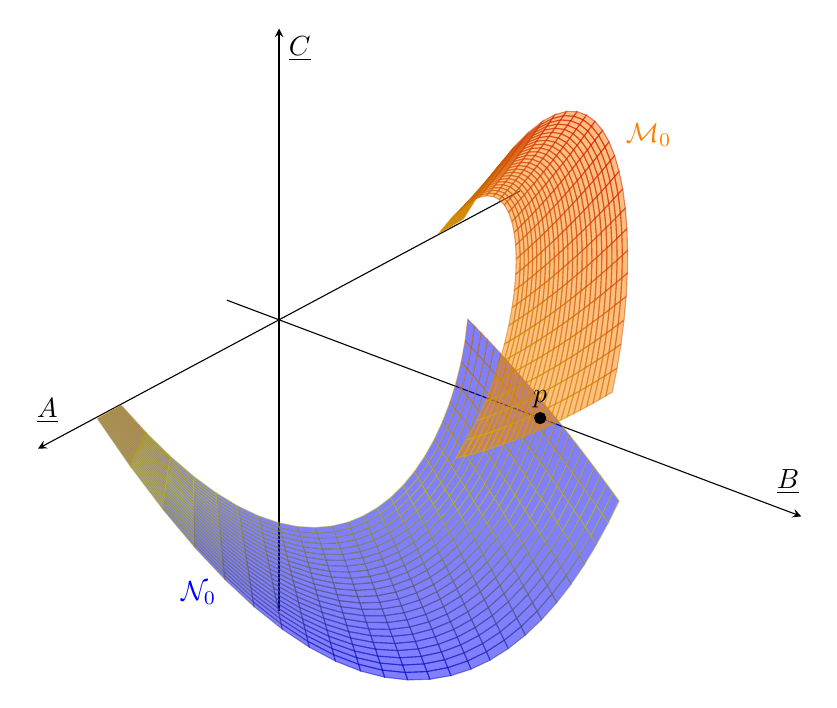
\begin{tikzpicture}
		\begin{axis}
			[
			axis lines = center,
			width=15cm,
			height=15cm,
			xmin = -1.0, xmax =1.0,
			ymin = -0.1, ymax= 1.0,
			zmin= -0.5, zmax=0.5,
			xtick style={draw = none},
			ytick style={draw = none},
			xticklabels={,,},
			yticklabels={,,},
			zticklabels={,,},
			ztick style={draw = none},
			xlabel=$\underline{A}$,
			ylabel=$\underline{B}$,
			zlabel=$\underline{C}$,
			view={130}{30},
			]
			\addplot3[surf,color= blue, opacity =0.5,
			domain=(0.7071 - 0.05 ):(0.7071 + 0.05), %omega
			domain y = 0.001:0.9, % t
			]
			({x*(1-y) - 0.1* y}, %
			{((-x^2 + 3*x^4 - (x*(1-y) - 0.1 * y)^2 + (x*(1-y) - 0.1 * y)^4 + 2*(x*(1-y) - 0.1 * 	y)*(x-2*x^3)))^(0.5)},
			{x - 2*x^3 - (x*(1-y) - 0.1 * y) + 2*(x*(1-y) - 0.1 * y)^3});
			\addplot3[surf,color= orange, opacity =0.5,
			domain=(-0.7071 - 0.05 ):(-0.7071 + 0.05), %omega
			domain y = 0.005:0.9, % t
			]
			({x*(1-y) + 0.1* y}, %
			{((-x^2 + 3*x^4 - (x*(1-y) + 0.1 * y)^2 + (x*(1-y) + 0.1 * y)^4 + 2*(x*(1-y) + 0.1 * y)*(x-2*x^3)))^(0.5)},
			{x - 2*x^3 - (x*(1-y) + 0.1 * y) + 2*(x*(1-y) + 0.1 * y)^3});
			\addplot3[mark=*,black,point meta=explicit symbolic,nodes near coords] 
			coordinates {(0,0.5,0)[$p$]};
			\addplot3[black,point meta=explicit symbolic,nodes near coords] 
			coordinates {(-0.45,0.5,0.35)[$\color{orange} {\mathcal M}_0$]};
			\addplot3[black,point meta=explicit symbolic,nodes near coords] 
			coordinates {(0.55,0.1,-0.35)[$\color{blue} {\mathcal N}_0$]};
		\end{axis}
	\end{tikzpicture}
	\caption{The above figure shows the stable and unstable manifolds for \(\epsilon = 0\). The manifolds \(\mathcal M_0\) and \(\mathcal N_0\) have a transverse intersection at \(p = (0,1/2,0)\).}
\end{figure}

Take \(\omega\) to be a point near \(A_{-\infty} = - 1/\sqrt 2\). The orbit that approaches \((\omega, 0, 0)\) in backwards time lies on the intersection of 
\begin{equation}
	\begin{aligned}
		I_1(\underline A, \underline B, \underline C) &= I_1(\omega, 0, 0) = \omega - 2\omega^3 \\
		I_2(\underline A, \underline B, \underline C) &= I_2(\omega, 0, 0) = - \frac 1 2 \omega^2 + \frac 3 2 \omega^4.
	\end{aligned}
\end{equation}
Setting \(\underline A = 0\), we can find that \(\mathcal M_0\) hits the \(\underline B \underline C\)- plane at 
\begin{equation}
	m(\omega) = (0, |\omega| \sqrt{3\omega^2 -1 }, \omega - 2\omega^3)
\end{equation}
for \(\omega\) close to \(A_{-\infty}\). In particular, we see \(m(A_{-\infty}) = p\). Identical reasoning gives that \(\mathcal N_0\) intersects the plane at 
\begin{equation}\label{intersection-with-plane}
	n(\alpha) = (0, |\alpha| \sqrt{3\alpha^2 -1 }, \alpha - 2\alpha^3)
\end{equation}
where \(\alpha\) is near \(A_\infty = 1 / \sqrt 2\) and \(n (A_{\infty} ) = p\).

A tangent vector to the heteroclinic orbit is given by \(\gamma_{+}'(0) = (1/2, 0, -1/2)\), and this vector lies in both \(T_p\mathcal M_0\) and \(T_p \mathcal N_0\). Since \(m(\omega) \in \mathcal M_0\) for \(\omega\) near \(A_{-\infty}\), we have that 
\begin{equation}
	m'(A_{-\infty}) = \left( 0, 1, \frac  1 {\sqrt 2} \right) \in T_p \mathcal M_0.
\end{equation}
Similarly,
\begin{equation}
	n'(A_{\infty}) = \left( 0, 1, \frac  {-1} {\sqrt 2} \right) \in T_p \mathcal N_0.
\end{equation}
Therefore
\begin{equation}
	T_p \mathcal M_0 + T_p \mathcal N_0 = \mathrm{span} \left\{ \left(\frac 1 2 , 0, \frac{-1} 2\right),  \left( 0, 1, \frac  1 {\sqrt 2} \right) ,  \left( 0, 1, \frac  {-1} {\sqrt 2} \right) \right\} = T_p\R^3
\end{equation}
and the intersection is transverse. This implies that there is a heteroclinic orbit on the intersection of \(\mathcal M_\epsilon\) and \(\mathcal N_\epsilon\) for \(\epsilon > 0\). 


\subsection{Estimates on the heteroclinic orbit}

From the previous section, we have the existence of heteroclinic orbits that are perturbation of \(\gamma_\pm\) at \(\epsilon = 0\). From the \(C^1\) regularity of the manifolds with respect to the coordinates, we expect that the orbits remain \(\mcO(\epsilon)\) close to the unperturbed orbits in some sense. There are some subtleties to be addressed. The manifolds remain \(\mcO(\epsilon)\) close in Hausdorff distance, but this does not imply the orbits on the manifolds remain \(\mcO(\epsilon)\) close for all time. The dynamics on the manifolds might change causing orbits on the perturbed manifold to diverge asymptotically despite remaining close initially.

First, let us introduce notation for the perturbed heteroclinic orbits. We shall denote by \(\gamma_{\pm, \epsilon} = (A_{\pm, \epsilon} , B_{\pm, \epsilon}, C_{\pm,\epsilon})\) the perturbations of \(\gamma_{\pm}\) for \(\epsilon > 0\), where we set \(\gamma_{\pm,\epsilon}(0)\) to be the point where the orbits cross the \(\underline{B}\underline{C}\)-plane. From the continuity of the manifolds with respect to \(\epsilon\), we have that \(|\gamma_{\pm, \epsilon}(0) - \gamma_\pm(0)| = \mcO(\epsilon)\) for small \(\epsilon\). We can extend this estimate onto arbitrarily large finite time scales by applying an argument using the Gr\"onwall inequality. That is, for every \(T> 0\) we have for sufficiently small \(\epsilon\) that \(|\gamma_{\pm, \epsilon}(s) - \gamma_\pm(s)| = C\epsilon\) for all \(s\in[-T,T]\), where \(C>0\) is independent of \(s\). 

This argument is insufficient for extending the estimate to all time. To get that the orbits remain close as \(s\to\pm\infty\), we can rely on part 7 of \cref{foliation-of-unstable-manifold}. Checking the values of the generalized Lyapunov-type numbers, we can see that at \(p = (A_{-\infty}, 0, 0, 0)\), we have that
\begin{equation}
	\sigma^{cu}(p_0) = \exp(-\sqrt{6 A_{-\infty}^2 -1}), \quad \sigma^{su}(p_0) = \exp(-2\sqrt{6 A_{-\infty}^2 -1}).
\end{equation}
Then if we make the manifold small enough, this condition for the hypotheses of \cref{foliation-of-unstable-manifold} hold. We check that this condition is not broken by perturbation of the vector field with the bump function in \cref{condition-verification}. Taking \((\epsilon, \omega)\) sufficiently close to \((0, A_{-\infty})\) as base points, the theorem states that the unstable manifold is \(C^1\) with respect to \((\epsilon, \omega)\). Note that the overflowing invariant manifold (away from the bump function) consists only of fixed points, so orbits on the unstable manifold approach a unique fixed point given by \((\epsilon, \omega)\). Take \(T> 0\) large enough so that all the points on \(\mathcal M_\epsilon\) (for \(\epsilon \leq \epsilon_0\)) which intersect the \(\underline B \underline C\)-plane are in the local unstable manifold when flowed backward in time by \(-T\) units. Then locally, there is a one-to-one correspondence between these points flowed backward in time and the points in \(\overline M\); furthermore, this correspondence is \(C^1\) due to \cref{foliation-of-unstable-manifold}. This implies that if the points flowed backward are \(\mcO(\epsilon)\) close then their backward limits are \(\mcO(\epsilon)\) close as well. In particular, the backward limits of \(\gamma_{+,\epsilon}\) and \(\gamma_+\) are \(\mcO(\epsilon)\) close. The argument for the stable manifold is analogous. This shows that the heteroclinic orbits remain \(\mcO(\epsilon)\) close for all time. In the case where \(V(x) = \frac 12 x^2 - \frac 1 {24} x^4 + \mcO(\epsilon^6)\), this can be upgraded to \(\mcO(\epsilon^2)\); the proof is similar but we use the regularity of the manifolds with respect to \(\eta = \epsilon^2\) instead. Therefore, we have the following.
\begin{prop}
	There exists \(\epsilon_0 > 0\) such that for every \(\epsilon\in(0,\epsilon_0]\) there exist two heteroclinic orbits \(\gamma_{\pm, \epsilon}\) of \cref{epsilon-flow} such that 
	\begin{equation}
		|\gamma_{\pm,\epsilon}(s) - \gamma_\pm(s) | \leq C \epsilon \quad \text{ for all } s\in \R
	\end{equation}
	where \(\gamma_{\pm}\) are defined in \cref{heteroclinic-orbit-at-zero}. If \(V\) satisfies (H2), then we instead have the estimate
	\begin{equation}
		|\gamma_{\pm,\epsilon}(s) - \gamma_\pm(s) | \leq C \epsilon^2 \quad \text{ for all } s\in \R.
	\end{equation}
\end{prop}

By starting to unravel the change of coordinates, we can show the existence of solutions to the advance-delay equation of the form
\begin{equation}
	x_{\pm,\epsilon}(t) = q_{\pm, \epsilon}(t) + (\Phi_\mu(\epsilon A_{\pm, \epsilon}(\epsilon t),\epsilon^2 B_{\pm, \epsilon}(\epsilon t) ,\epsilon^3 C_{\pm, \epsilon}(\epsilon t))_x
\end{equation}
where \(q_{\pm, \epsilon}(t)\) satisfies the differential equation
\begin{equation}
	\frac{dq_{\pm, \epsilon}}{dt} =  \epsilon A_{\pm, \epsilon}(\epsilon t).
\end{equation}
The differential equation for \(q\) comes from \cref{ode-for-q} and the fact that \(\zeta_1^*(\Phi_\mu) = 0\). Using the fact that for solutions of \cref{first-order-abstract-ode} satisfy \(\partial_t (U)_x = U_\xi\), we also have that
\begin{equation}
	\dot x_{\pm, \epsilon}(t) =  \epsilon A_{\pm, \epsilon}(\epsilon t) + (\Phi_\mu(\epsilon A_{\pm, \epsilon}(\epsilon t),\epsilon^2 B_{\pm, \epsilon}(\epsilon t) ,\epsilon^3 C_{\pm, \epsilon}(\epsilon t))_\xi.
\end{equation}
The coordinates \(A_{\pm, \epsilon}\), \(B_{\pm, \epsilon}\), and  \(C_{\pm, \epsilon}\) are at least \(C^5\) and \(\Phi_\mu\) is at least \(C^4\) in its spatial variables.

The main result will be stated by writing \cref{fput-lattice-odes} in terms of the strain variables, \(u_n = x_{n+1} - x_n\). That is, we look at the traveling wave solution given by 
\begin{equation}
	x_{\pm, \epsilon}(n+1-c\tilde t) - x_{\pm, \epsilon}(n-c\tilde t).
\end{equation}
Using a Taylor series expansion centered at \(t + \frac 12 \) for \( x_{\pm, \epsilon}(t+ 1)\) and \( x_{\pm, \epsilon}(t)\), we get 
\begin{align}
	& x_{\pm, \epsilon}(t+ 1/2) + \frac 12 \dot x_{\pm, \epsilon}(t+1/2) + \frac 1 8\ddot x_{\pm, \epsilon}(t+1/2) + \frac 1 2\int_{0}^{1/2} \dddot x_{\pm, \epsilon}(t+1/2+s)(s-1/2)^2 \, ds \\
	& x_{\pm, \epsilon}(t+ 1/2) - \frac 12 \dot x_{\pm, \epsilon}(t+1/2) + \frac 1 8 \ddot x_{\pm, \epsilon}(t+1/2) - \frac 1 2\int_0^{1/2} \dddot x_{\pm, \epsilon}(t+s)s^2 \, ds 
\end{align}
respectively for each term. Thus 
\begin{equation}
\begin{aligned}
	&x_{\pm, \epsilon}(t+1) - x_{\pm, \epsilon}(t) \\
	&\quad= \dot x_{\pm, \epsilon}(t+ 1/2) + \frac 12 \int_{0}^{1/2} [\dddot x_{\pm, \epsilon}(t+1/2+s)(s-1/2)^2 - \dddot x_{\pm, \epsilon}(t+s)s^2] ds \\
	&\quad= \pm \epsilon \varphi_1(\epsilon (t+1/2)) + \epsilon^2 \mathcal R_{\epsilon, \pm}(\epsilon (t+1/2))
\end{aligned}
\end{equation}
where \(R_{\epsilon, \pm} \in C^3_b\). Thus (after shifting the solution) we have that there are traveling wave like solutions of the FPUT of the form
\begin{equation}
	u_n(t) = \pm \epsilon \varphi_1(\epsilon(n-ct)) + \epsilon^2 \mathcal R_{\epsilon, \pm}(\epsilon (n-ct))
\end{equation}
Additionally, if (H2) holds we improve the error estimate so that there are solutions of the form 
\begin{equation}
	u_n(t) = \pm \epsilon \varphi_1(\epsilon(n-ct)) + \epsilon^3 \mathcal R_{\epsilon, \pm}(\epsilon (n-ct)).
\end{equation}

To match similar estimates made in \cite{friesecke1999solitary}, one would expect the remainder terms to also be in a Sobolev space like \(H^1\). This is in general not true. The traveling wave solution found above may approach a different limit asymptotically than \(\epsilon \varphi_1 \), in which case the remainder does not approach zero asymptotically in space. A necessary condition to get \(\mathcal R_{\epsilon,\pm}\in H^1\) would be for \(u_n\) to approach the same limits of \(\pm \epsilon \varphi_1(\epsilon (n-ct))\) as \(|n| \to \infty\).

A useful tool for showing this is the following invariant for \cref{advance-delay-equation}:
\begin{equation}\label{advance-delay-invariant}
	\dot x(t) - \mu \int_t^{t+1} V'(x(s) - x(s-1)) \, ds.
\end{equation}
It is easy to check that the above is constant for solutions of the advance-delay differential equation. If \(\dot x(t) \to r_\infty\) as \(t\to \infty\), then \cref{advance-delay-invariant} is equal to 
\begin{equation}
	r_\infty - \mu V'(r_\infty)
\end{equation}
If we also have that \(\dot x(t) \to r_{-\infty}\) as \(t\to-\infty\), then we have \cref{advance-delay-invariant} is also equal to 
\begin{equation}
	r_{-\infty} - \mu V'(r_{-\infty}) 
\end{equation}
and so the limits \(r_{\pm \infty}\) satisfy the equation
\begin{equation}
	r_\infty - \mu V'(r_\infty) = r_{-\infty} - \mu V'(r_{-\infty}) .
\end{equation}
For arbitrary \(V\), we cannot show that the limits agree with the limits of \(\pm\epsilon \phi \). However, if we assume (H3) holds, i.e.\ that \(V(x) = \frac 1 2 x^2 - \frac 1 {24} x^4\), then we do have the limits agree. This follows in part from the oddness of \(V'\) and the reversibility of the system. Recall that the vector field on the center manifold is reversible (given by the reversibility operator \(S_0\)) and odd. Therefore, we have that
\begin{equation}
	\begin{bmatrix}
		- A_{\pm, \epsilon} (-s) \\
		B_{\pm, \epsilon} (-s) \\
		-C_{\pm, \epsilon} (-s)
	\end{bmatrix}
\end{equation}
is also a solution on the center manifold. One can note that the above solutions lie on the intersection of the stable and unstable manifolds and are in an \(\epsilon\)-neighborhood of the unperturbed heteroclinic orbits \(\gamma_{\pm}(s)\). This contradicts the uniqueness of the transverse intersection of the manifolds in a neighborhood of the original intersection, and thus the above solutions must in fact be \(\gamma_{\pm,\epsilon}(s)\). Hence, comparing the limits at infinity we have that \(\lim_{s\to\infty} A_{\pm,\epsilon} (s) = -\lim_{s\to-\infty} A_{\pm, \epsilon}(s)\) and so \(r_\infty = - r_{-\infty}\). Therefore, we must have that 
\begin{equation}
	r_\infty - \mu V'(r_\infty) = 0.
\end{equation}
Given that \(V'(x) = x - \frac 1 6 x^3\), we have that the only solutions to the above equation are \(r_{\infty} = 0, \pm \epsilon / \sqrt 2\). This implies that the limits of the traveling wave solutions agree with \(\pm \epsilon \phi\). Specifically, we must have \(A_{\pm, \epsilon}(s) \to \pm 1 / \sqrt 2\) as \(s\to \infty\) and \(A_{\pm, \epsilon}(s) \to \mp 1 / \sqrt 2\) as \(s\to -\infty\).

Now to get the Sobolev estimate, we use the following lemma.
\begin{restatable}{lem}{heteroclinicorbitsobolev}\label{heteroclinic-orbit-sobolev}
	Suppose that (H3) holds. Then there exist \(C> 0\) and \(\alpha > 0\) such that
	\begin{equation}
		| \gamma_{\pm, \epsilon}(s) - \gamma_{\pm}(s) | \leq C e^{-\alpha| s|} \epsilon.
	\end{equation}
	Furthermore, the difference of the heteroclinic orbits are in \(H^5(\R; \R^3)\) and 
	\begin{equation}
		\| \gamma_{\pm, \epsilon}(s) - \gamma_{\pm}(s) \|_{H^5(\R;\R^3)}  \leq C \epsilon.
	\end{equation}
\end{restatable}
The proof of \cref{heteroclinic-orbit-sobolev} is given in \cref{lemma-appendix}. Thus we have
\begin{equation}
	\|A_{\pm, \epsilon} \mp \varphi_{1}\|_{H^5(\R;\R)} \leq C \epsilon.
\end{equation}
One can also show from the exponential decay of \(\gamma_{\pm, \epsilon}\) and the smoothness of \(\Phi_\mu\) that
\begin{equation}
	(\Phi_\mu(\epsilon A_{\pm, \epsilon}(s),\epsilon^2 B_{\pm, \epsilon}(s) ,\epsilon^3 C_{\pm, \epsilon}(s))_\xi \in H^4(\R;\R).
\end{equation}
By noticing that the Taylor expansion of \(\Phi_\mu(\epsilon A_{\pm, \epsilon}, \epsilon^2 B_{\pm, \epsilon}, \epsilon^3 C_{\pm, \epsilon})\) has no terms of order \(\epsilon^2\) or lower, the function is at least of order \(\epsilon^3\). Therefore, we have that there is an \(R_{\pm,\epsilon} \in H^4(\R;\R)\) such that
\begin{equation}
	\dot x_{\pm, \epsilon }(t) = \pm \epsilon\varphi_1(\epsilon t) + \epsilon^2 R_{\pm,\epsilon}(\epsilon t).
\end{equation}
Then converting to strain coordinates as before we have
\begin{equation}
	u_n(t) = \pm\epsilon\varphi_1(\epsilon(n-ct)) + \epsilon^2 \mathcal R_{\pm, \epsilon}(\epsilon(n-ct))
\end{equation}
where \(\mathcal R_{\pm, \epsilon} \in H^3(\R;\R)\).

We state our results as follows.
\begin{theorem}\label{thm:estimates-on-profile}
	There exists \(\epsilon_0> 0\) and \(C> 0\) such that for every \(\epsilon > (0,\epsilon_0]\) there is a traveling wave solution given by \(u_n(t) = u_c(n-ct)\) with positive wave speed \(c^2 = 1 - \epsilon^2/12\). Furthermore, we have the additional estimates on the wave profile of \(u_c\).
	\begin{enumerate}[label = (\roman*)]
		\item If (H1) holds, then
		\begin{equation}
			\left\| \frac 1 \epsilon u_c\left(\frac \cdot \epsilon \right) - \varphi_1 \right\|_{C^3} \leq C \epsilon
		\end{equation}
		\item If (H2) holds, then
		\begin{equation}
			\left\| \frac 1 \epsilon u_c\left(\frac \cdot \epsilon \right) - \varphi_1 \right\|_{C^3} \leq C \epsilon^2
		\end{equation}
		\item If (H3) holds, then
		\begin{equation}
			\left\| \frac 1 \epsilon u_c\left(\frac \cdot \epsilon \right) - \varphi_1 \right\|_{H^3} \leq C \epsilon
		\end{equation}
	\end{enumerate}
\end{theorem}
The same estimates hold for \(-\varphi_1\) as the profile wave or for left-moving waves or for both.
	\cleardoublepage
	
	% -------------------------------------
	% CHAPTER ?: LONG-TIME STABILITY OF SMALL FPU SOLITARY WAVES
	% -------------------------------------
	% !TeX root = ../thesis.tex
\chapter{Long-Time approximations of small-amplitude, long-wavelength  FPUT solutions}
\label{chp:long-time-stability}
\pagestyle{myheadings}

\section{Introduction}

As shown in earlier work, there exists a wave solution of the FPUT lattice whose profile is well approximated by that of the kink solution to the (defocusing) mKdV. This approximation holds globally in time, but is restricted to one special solution of the FPUT. We are now interested in studying more general solutions of the FPUT which can be approximated by solutions of the mKdV for long (but finite) time. The equations of motion on the lattice are given by 
\begin{equation*}
	\ddot x_n = V'(x_{n+1} - x_n) - V'(x_n - x_{n-1}), \quad n \in \Z. \tag{\ref{fput-lattice-odes}}
\end{equation*}
where \(V\) is the interaction potential between neighboring particles and \(\dot{\hspace{0.5em}}\) denotes the derivative with respect to the time \(t\in \mathbb{R}\). \Cref{fput-lattice-odes} can be rewritten in the strain variables \(u_n := x_{n+1} - x_n\) as follows
\begin{equation*}
	\ddot{u}_n = V'(u_{n+1}) - 2 V'(u_n) + V'(u_{n-1}), \quad n \in \Z \tag{\ref{fput-lattice-equations-strain-variables}}
\end{equation*}
The moving wave solution in \cref{fput-lattice-odes} corresponds to a kink-like solution in \cref{fput-lattice-equations-strain-variables}.

For the case where \(V\) is of the form \(V(u) = \frac 1 2 u^2 + \frac{\epsilon^2}{p+1} u^{p+1}\) for \(p\geq 2\), the generalized KdV equation given by 
\begin{equation}\label{generalized-KdV}
	2 \partial_TW + \frac 1 {12} \partial_X^3 W + \partial_X(W^p) = 0,\quad X\in\R
\end{equation} 
serves as a modulation equation for solutions of \cref{fput-lattice-equations-strain-variables} \cite{bambusi2006metastability,friesecke1999solitary}. That is, for a local solution \(W\in C([-\tau_0,\tau_0],H^s(\R))\) of \cref{generalized-KdV} there exist positive constants \(\epsilon_0\) and \(C_0\) such that, for all \(\epsilon \in (0,\epsilon_0)\), when initial data \((u_{\mathrm{in} }, \dot u_{\mathrm{in}})\in\ell^2(\R)\) satisfy
\begin{equation}
	\|u_{\mathrm{in}} - W(\epsilon\cdot, 0) \|_{\ell^2} + \| \dot u_{\mathrm{in}} + \epsilon \partial_X W(\epsilon\cdot, 0) \|_{\ell^2} \leq \epsilon^{3/2},
\end{equation}
the unique solution to \cref{fput-lattice-equations-strain-variables} with initial data \((u_{\mathrm{in} }, \dot u_{\mathrm{in}})\) belongs to \(C^1([-\tau_0\epsilon^{-3}, \tau_0 \epsilon^{-3}];\allowbreak \ell^2(\Z))\) and satisfies 
\begin{multline}
	\|u(t) - W(\epsilon (\cdot - t),\epsilon^3 t)\|_{\ell^2(\Z)} + \| \dot u(t) + \epsilon \partial_X W(\epsilon(\cdot - t), \epsilon^3 t) \|_{\ell^2(\Z)} \leq C_0 \epsilon^{3/2}, \\ t\in[-\tau_0 \epsilon^{-3},\tau_0 \epsilon^{-3}].
\end{multline}
Furthermore, the approximation can also be extended to include counter-propagating solutions of the KdV in the case where \(p=2\) \cite{schneider2000counter,hong2021korteweg}.

The KdV approximation was extended to longer time scales on the order of \(\epsilon^{-3}|\log(\epsilon)|\) by Khan and Pelinovsky in order to deduce the nonlinear metastability of small FPUT solitary waves from the orbital stability of the corresponding KdV solitary waves \cite{khan2017long}.

We consider the FPUT with potential
\begin{equation}\label{truncated-potential}
	V(u) = \frac 1 2 u^2 - \frac{1} {24} u^4.
\end{equation}
This potential differs from those studied in \cite{khan2017long} in that it admits kink solutions. Numerical experiments show that these kink solutions play an important role in the FPUT recurrence for lattices with potential give in \cref{truncated-potential} \cite{pace2019beta}. We will introduce an ansatz that solutions of the FPUT with this potential can be well-approximated by counter-propagating solutions of mKdV equations.

The technique of the proof follows from ideas in \cite{schneider2000counter,khan2017long} and is roughly sketched out as follows. First the system is rewritten into a Hamiltonian system on a Hilbert space, \(H\):
\begin{equation}\label{hamiltonian-system}
	\dot X(t) = J \mcH'(X)
\end{equation}
where \(J:H\to H\) is a skew symmetric operator and \(\mcH\) is the Hamiltonian such that \(\mcH'(X) = LX + N(X)\) with \(L:= \mcH'(0)\). We introduce some ansatz \(\tilde X_\epsilon\) which is an approximate solution to \cref{hamiltonian-system} in the sense that 
\begin{equation}
	\mathrm{Res}(t) := J[L\tilde X_\epsilon(t)  + N(\tilde X_\epsilon(t))] - \dot{\tilde {X_\epsilon}}(t) 
\end{equation}
has norm of order \(\epsilon^\alpha\) for \(\alpha > 0\)  for all time \(t\). The approximate solution will be ``small-amplitude" in the sense that \(\| \tilde X_\epsilon \| = \mathcal O(\epsilon^k)\) for \(k > 0 \). Then we can write the evolution equation for the \(R(t) = X(t) - \tilde X_\epsilon(t)\) as 
\begin{equation}\label{hamiltonian-system-2}
	\dot R(t) = J[L + N'(\tilde X_\epsilon(t))]R(t) + \mathrm{Res}(t) + \mathcal N(\tilde X_\epsilon, R)
\end{equation}
with \(\mathcal N( X_\epsilon, R) := J[N(\tilde X_\epsilon +R) - N(\tilde X_\epsilon) - N'(\tilde X_\epsilon)R]\). The goal is then to show that \(R(t)\) remains small for long periods of time so that the approximation \(X \approx \tilde X_\epsilon\) is valid for that time. The standard way to prove this is to find a suitable energy function to control the norm of \(R\) with. If \(L + N'(\tilde X_\epsilon(t))\) is self-adjoint, then \cref{hamiltonian-system-2} is up to first order a linear, non-autonomous, Hamiltonian system with Hamiltonian \(\mcH_1(R, t) = \frac 1 2 \langle (L+N'(\tilde X_\epsilon)) R, R\rangle\). Therefore, \(\mcE(t) := \mcH_1(R(t),t)\) serves as a natural choice of energy function for \cref{hamiltonian-system-2}. Hence, if one shows that \( \| R\|^2\lesssim\mcE(t)\) and that  \(\|\mathcal N(\tilde X_\epsilon, R) \| \lesssim \epsilon^{k+2} \mcE(t)\), then can show that \(\mcS(t) = \mcE(t)^{1/2}\) satisfies
\begin{equation}
	|\dot \mcS (t) | \lesssim \epsilon^{\alpha} + \epsilon^{k+2}\mcS(t).
\end{equation}
Intuitively, one would expect \(\mcS(t)\) to grow like \(\mcS(t) \sim \epsilon^\alpha t + e^{\epsilon^{k+2} t} \mcS(0)\). Taking \(\mcS(0) =\epsilon^\gamma\) for \(\gamma \geq 1\) and assuming \(\alpha > 2(k+2)\), we have \(\mcS(t) \sim \epsilon^\gamma \) for \(|t|\lesssim \epsilon^{-(k+2)}\). One can further the time where the approximation holds by relaxing how big \(\mcS(t)\) can get. Taking \(r>0\) small, one can show that \(\mcS(t) \sim \epsilon^{\gamma - r}\) for \(|t| \lesssim r \epsilon^{-(k+2)}|\log(\epsilon)|\).

%Something about metastability here.

\section{Counter-Propagating Waves Ansatz}

%Write out counter-propagting ansatz for solution 
We make the assumption that solutions of \cref{fput-lattice-equations-strain-variables} can be expressed as a sum of two counter-propagating small-amplitude waves, i.e., 
\begin{equation}\label{ansatz}
	u_n(t) \approx \epsilon f(\epsilon(n+t), \epsilon^3t) + \epsilon g(\epsilon(n-ct), \epsilon^3 t) + \epsilon^3\phi(\epsilon n, \epsilon t)
\end{equation}
where we allow \(f\) to have a fixed non-zero limits, \(f_{\pm\infty}\), at positive and negative infinity and \(\phi\) captures the interaction effects between \(f\) and \(g\). The wave speed of \(g\) is given by
\begin{equation}\label{ansatz-wave-speed}
	c = c(\epsilon, f_\infty) = 1 - \frac{\epsilon^2 f_\infty^2}{4}.
\end{equation}
Plugging in the ansatz in \cref{ansatz} back into \cref{fput-lattice-equations-strain-variables} and grouping terms of the same order \(\epsilon\) together gives
\begin{equation}
	\begin{aligned}
		&\epsilon^3 \Big(\partial_1^2 f(\cdot, \epsilon^3 t) + \partial_1^2 g(\cdot, \epsilon^3 t)\Big) \\
		&+ \epsilon^5 \Big( 2 \partial_1\partial_2 f(\cdot, \epsilon^3t) - 2 \partial_1\partial_2 g(\cdot, \epsilon^3 t) - \frac{f_\infty^2} 2 \partial_1^2 g + \partial_2^2 \phi(\epsilon x, \epsilon t)\Big) \\
		&+ \mathcal O(\epsilon^6)\\
		&\qquad = \quad \epsilon^3 \Big(\partial_1^2 f(\cdot, \epsilon^3 t) + \partial_1^2 g(\cdot, \epsilon^3 t)\Big) \\
		&\qquad\qquad + \epsilon^5\Big(\partial_1^2  \phi(\epsilon x, \epsilon t) \\
		&\qquad\qquad\qquad - \frac 1 6 \partial_1^2 \big[f^3(\cdot, \epsilon^3 t ) + 3 f^2(\cdot,\epsilon^3)g(\cdot, \epsilon^3t) + 3 f(\cdot, \epsilon t) g^2(\cdot,\epsilon^3 t) + g^3(\cdot, \epsilon^3 t)\big] \\
		&\qquad\qquad\qquad+ \frac 1 {12} \partial_1^4 f(\cdot, \epsilon^3 t) + \frac 1 {12} \partial_1^4 g(\cdot, \epsilon^3 t)\Big) \\
		&\qquad\qquad+ \mathcal O(\epsilon^6).
	\end{aligned}
\end{equation}
Clearly the equation will hold up to order \(\epsilon^3\). For the order \(\epsilon^5\) terms, the equation will again hold if \(f\), \(g\), and \(\phi\) satisfy
\begin{equation}\label{f-mKdV}
	2 \partial_2 f = - \frac 1 6 \partial_1(f^3) + \frac 1 {12} \partial_1^3 f
\end{equation}
and 
\begin{equation}\label{g-gKdV}
	-2 \partial_2 g = - \frac 1 6 \partial_1 (g^3 + 3f_\infty g^2) + \frac 1 {12}\partial_1^3 g,
\end{equation}
and
\begin{equation}\label{phi-pde}
	\begin{aligned}
		\partial_2^2 \phi(\xi, \tau) = \partial_1^2\phi(\xi, \tau)- \frac 1 6 \partial_1^2 \big[& 3(f^2(\xi+\tau,\epsilon^2\tau)-f_\infty^2)g(\xi-c\tau,\epsilon^2\tau) \\&+ 3 (f(\xi+\tau,\epsilon^2\tau)-f_\infty)g^2(\xi-c\tau,\epsilon^2\tau) \big ] \\
		\phi(\xi,0) = \partial_1 \phi(\xi, 0) = 0.
	\end{aligned}
\end{equation}
Note that \cref{f-mKdV} is the defocusing mKdV equation and \cref{g-gKdV} is a type of generalized KdV equation. This formal calculation shows that the mKdV can serve as a modulation equation. That is, for \(\epsilon\) sufficiently small, one would expect the ansatz in \cref{ansatz} to hold for time on the order of \(\epsilon^{-3}\). We make precise this notion, but we must first make decisions for the function spaces in which the functions \(f\), \(g\), and \(\phi\) must live.

A natural choice of function space for \(g\) is a Sobolev space like \(H^k(\R)\). However, for \(f\), we want to allow the possibility of the function approaching a non-zero limit at positive and negative infinity while also having sufficient regularity. 
\begin{defn}
	For \(k\in\N\), let \(\mcX^k(\R)\) be the Banach space 
	\begin{equation}
		\mcX^k(\R) := \{f \in L^\infty(\R) \mid f'\in H^{k-1}(\R)\}
	\end{equation}
	with norm
	\begin{equation}
		\| f \|_{\mcX^k(\R)} := \| f \|_{L^\infty(\R)} + \| f' \|_{H^{k-1}(\R)}.
	\end{equation}
\end{defn}
Then \(\mcX^k\) is the set of \(L^\infty\) functions which are \(k\) times weakly differentiable and whose derivatives are in \(L^2\). That this is a Banach space follows from the Banach space isomorphism
\begin{equation}
	\mcX^k(\R) \cong L^\infty(\R) \cap \dot H^1(\R) \cap \dot H^k(\R),
\end{equation}
where \(\dot H^k(\R)\) denotes the homogeneous Sobolev spaces. For convenience, we let \(\mcX^0(\R)\) denote \(L^\infty(\R)\)

Note that \cref{f-mKdV} has kink solutions of the form
\begin{equation}\label{kink-solutions}
	f(X,T) = - \sqrt{12 v} \tanh\left( \sqrt{12v} (X-vT)\right).
\end{equation}
In particular, setting \(v = 24\) we get the approximate solution on the lattice given by
\begin{equation}
	- \frac \epsilon {\sqrt 2} \tanh\left(\frac \epsilon {\sqrt 2} \left(n + \left(1-\frac{\epsilon^2} {24}\right) t\right)\right),
\end{equation} which seems to agree with the kink solution on the lattice for long periods of time (i.e.\ it should hold formally for \(t\) of order \(\mathcal O(\epsilon^{-4})\)). The space \(\mcX^k\) allows for \(f\) to be these kink solutions and thus allows us to study the kink solution of the lattice found previously. 

We also have the following inequalities for products of functions in \(\mcX^k\) and \(H^k\) that will be useful. 

	
\begin{restatable}{lem}{prodruleone}
	\label{prod-rule-1-lem}
	For non-negative integers \(k\), there is a \(C>0\) such that
	\begin{equation}\label{prod_rule}
		\| fg \|_{H^k} \leq C \| f \|_{\mathcal X^k} \| g \|_{H^k}
	\end{equation}
	for any \(f\in \mcX^k(\mathbb R)\) and \(g \in H^k(\mathbb R)\).
\end{restatable}

\begin{restatable}{lem}{prodruletwo}
	\label{prod-rule-2-lem}
	For non-negative integers \(k\), there is a \(C>0\) such that
	\begin{equation}\label{prod_rule_2}
		\| fg \|_{\mcX^k} \leq C \| f \|_{\mcX^k} \| h \|_{\mcX^k}
	\end{equation}
	for any \(f,g\in \mcX^k(\mathbb R)\).
\end{restatable}
See \cref{lemma-appendix} for proofs.

However, for our main result, we require that \(\phi\), the term which captures the interaction effects, remains uniformly bounded for all time. Intuitively, if \(f\) and \(g\) are localized, the inhomogeneous term in \cref{phi-pde} will quickly go to zero, and the equation governing \(\phi\) \cref{phi-pde} will approach the homogeneous wave equation, for which Sobolev norms remain uniformly bounded. Since the two functions are localized and counter-propagating, their product will quickly decay in time as the two wave profiles move in opposite directions. Thus we require that \(f\) and \(g\) quickly decay to their respective limits at infinity. This is enforced by assuming the functions belong to appropriate weighted Banach spaces.

\begin{figure}[h]
	\center
	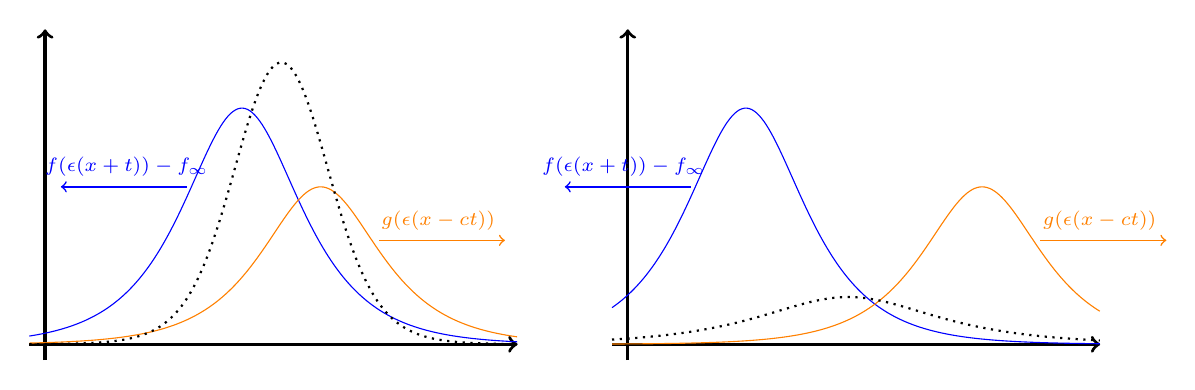
\begin{tikzpicture}[
		scale=2,
		declare function={sech(\x) = 2/(exp(\x) + exp(-\x));
			fun1(\x,\c) = 1.5 * sech((\x-\c)*3;
			fun2(\x,\c) = sech((\x-\c)*3);
		},
		]
		%axis
		\draw[->, very thick] (-0.1,0) -- (3,0) {};
		\draw[->, very thick] (0,-0.1) -- (0,2) {};
		
		%functions
		\draw[domain=-.1:3, samples = 200, color=blue] plot (\x, {fun1(\x, 1.25)} );
		\draw[domain=-.1:3, samples = 200, color=orange] plot (\x, {fun2(\x, 1.75)} );
		\draw[domain=-.1:3, samples = 200, thick, dotted] plot (\x, {2* fun1(\x,1.25) * fun2(\x,1.75)});
		
		%arrows
		\draw[->,line width=0.20mm,color=blue] (.9, 1) -- (0.1,1) {} node[above right] {\scriptsize\hspace{-1.5em} $f(\epsilon(x+t)) - f_\infty$};
		\draw[->,line width=0.20mm,color=orange] (2.12, .66) -- (2.92,.66) {} node[above left] {\scriptsize $g(\epsilon(x-ct))$};
		
		\begin{scope}[xshift=3.7cm]
			%axis
			\draw[->, very thick] (-0.1,0) -- (3,0) {};
			\draw[->, very thick] (0,-0.1) -- (0,2) {};
			
			%functions
			\draw[domain=-.1:3, samples = 200, color=blue] plot (\x, {fun1(\x, .75)} );
			\draw[domain=-.1:3, samples = 200, color=orange] plot (\x, {fun2(\x, 2.25)} );
			\draw[domain=-.1:3, samples = 200, thick, dotted] plot (\x, {0.3 * sech((\x - 1.4)*2});
			
			%arrows
			\draw[->,line width=0.20mm,color=blue] (.4, 1) -- (-0.4,1) {} node[above] {\scriptsize \hspace{5em} $f(\epsilon(x+t)) - f_\infty$};
			\draw[->,line width=0.20mm,color=orange] (2.62, .66) -- (3.42,.66) {} node[above left] {\scriptsize $g(\epsilon(x-ct))$};
		\end{scope}
	\end{tikzpicture}
	\caption{\label{fig-counter-propogating-interaction} The function \(f(\epsilon(x+t)) -f_\infty\) (shown in blue) moves to the left while \(g(\epsilon(x-ct))\) (shown in orange) moves to the right. Since they are localized, the product (shown by the dotted line) will quickly decay in time.}
\end{figure}

A suitable choice of space for \(g\) is the weighted Sobolev spaces \(H^k_n(\R)\). Here, \(H^k_n\) for \(k,n\in\mathbb N\cup \{0\}\)
\begin{equation}
	H^k_n(\R) := \{ g\in H^k(\R) \mid   g\langle \cdot \rangle^n \in H^k \}
\end{equation}
where \(\langle x \rangle = \sqrt{1+x^2}\). The norm on this space is
\begin{equation}
	\| g \|_{H^k_n(\R)} := \|  g \langle \cdot \rangle^n\|_{H^k(\R)}.
\end{equation}
This space has the useful property that if \(g \in H^k_n\), then its Fourier transform, \(\hat g \), is in \(H^n_k\) and 
\begin{equation}
	c \| \hat g \|_{H^n_k} \leq \| g \|_{H^k_n} \leq C \| \hat g \|_{H^n_k}
\end{equation}
for \(c,C>0\) independent of \(g\).

We want an analogous space for \(f\), but allowing for non-zero limits at infinity. Let \(\langle\cdot \rangle_+ :\R \to \R\) be a smooth function such that
\begin{equation}
	\langle x \rangle_+ = \begin{cases} \langle x \rangle, & x>1 \\ 1, & x<0\end{cases}
\end{equation}
and \(\langle \cdot \rangle_+\) continued smoothly between \(0\) and \(1\) such that it is always greater than or equal to \(1\). Thus \(\langle \cdot \rangle_+\) is a function that only acts like \(\langle \cdot \rangle\) for numbers greater than \(1\). The function \(\langle \cdot \rangle_-\) is similarly defined but for numbers less than \(-1\).

\begin{defn}
	Define \(\mcX^k_{n^+} (\R)\) to be the Banach space of functions where 
	\begin{equation}
		\mcX^k_{n^+} (\R) := \{ f \in \mcX^k(\R) \mid \lim_{x\to\infty} f(x) = f_\infty\text{ and } (f-f_\infty)\langle\cdot\rangle_+^n \in \mcX^k(\R)\}
	\end{equation}
	with norm given by
	\begin{equation}
		\| f \|_{\mcX^k_{n^+}(\R)} := |f_\infty| + \|(f-f_\infty) \langle \cdot \rangle_+^n \|_{\mathcal X^k(\R)}
	\end{equation}
	Similarly, 
	\begin{equation}
		\mcX^k_{n^-} (\R) := \{ f \in \mcX^k(\R) \mid \lim_{x\to-\infty} f(x) = f_{-\infty}\text{ and } (f-f_{-\infty})\langle\cdot\rangle_-^n \in \mcX^k(\R)\}
	\end{equation}
	and 
	\begin{equation}
		\| f \|_{\mcX^k_{n^-}(\R)} := |f_{-\infty}| + \|(f-f_{-\infty}) \langle \cdot \rangle_-^n \|_{\mathcal X^k(\R)}
	\end{equation}
	Define \(\mcX^k_n(\R)\) to be the intersection of these Banach spaces. That is,
	\begin{equation}
		\mcX^k_n(\R) := \mcX^k_{n^+} (\R) \cap \mcX^k_{n^-} (\R), \quad \| f \|_{\mcX^k_{n} (\R)} := \|f\|_{\mcX^k_{n^+} (\R)} + \|f\|_{\mcX^k_{n^-} (\R)}.
	\end{equation}
\end{defn}
	That \(\mcX^k_{n^\pm}\) are Banach spaces follows from the fact that there exists a linear isomorphism between the Banach space \(\R\times \mcX^k\) and these spaces, which is given by
\begin{equation}
	(\alpha, f) \mapsto \alpha + f \langle \cdot \rangle^{-n}_{\pm}.
\end{equation}
One can show that the kink solutions as specified in \cref{kink-solutions} lie in \(\mcX^k_n\) for all \(k,n\geq 0\); the derivatives are smooth and decay exponentially to zero, and the kink solutions approach the limits \(\mp\sqrt{12v}\) exponentially fast. These spaces also contain bounded rational functions. For instance, the function \[1 + \frac 1 {x^2 +1}\] is in \(\mcX^k_2(\R)\) since it approaches its limit at infinity (which in this case is \(1\)) at a rate of \(\mathcal O(1/x^2)\), and its derivatives are in \(H^0_2(\R)\).

The definitions above are used to prove that \(\phi\) remains bounded for all time. The idea behind the proof is similar to that of \cite[Lemma~3.1]{schneider2000counter}. The following lemma will be useful in showing the decay in products of \(f-f_\infty\) and \(g\).
\begin{restatable}{lem}{cknormbound}
	For each \(k\geq 0\) and \(c > 0\), there exists \(C> 0\) depending only on \(k\) such that 
	\begin{equation}\label{Ck-bound}
		\left \| \frac 1 {\langle \cdot +\tau\rangle_+^2 \langle \cdot - c\tau \rangle^2} \right \|_{C^k} \leq C\, \sup_{x\in\mathbb R} \frac 1 {\langle x +\tau\rangle_+^2 \langle x -c \tau \rangle^2}.
	\end{equation}
	Furthermore,
	\begin{equation}\label{sup-integrable}
		\int_0^\infty \sup_{x\in\mathbb R} \frac 1 {\langle x +\tau\rangle_+^2 \langle x -c \tau \rangle^2}\, d\tau <\infty.
	\end{equation}
\end{restatable}
See \cref{lemma-appendix} for proof. 

We are now ready to prove that \(\phi\) (and its time derivative) remain uniformly bounded in time.
\begin{prop}
	Fix \(T_0> 0\) and suppose that \(f \in C([-T_0,T_0], \mcX_2^{k+1}(\R))\) and \(g \in C([-T_0,T_0], H^{k+1}_2(\R)) \), with \(k>2\) an integer. Also, suppose that \(f(X,T)\to f_\infty\) as \(X\to \infty\) for any \(T\in[-T_0,T_0]\). Then there exists a constant \(C>0\) such that 
	\begin{equation}\label{phi-bound}
		\sup_{t\in[-\epsilon^{-3}T_0,\epsilon^{-3}T_0]} \|\phi(\cdot,\epsilon t)\|_{H^k} \leq C \Bigg( \sup_{t\in[-\epsilon^{-3}T_0,\epsilon^{-3}T_0]} \left\{\| f(\cdot, \epsilon^3t) \|_{\mathcal X^{k+1}_{2}},  \| g(\cdot, \epsilon^3t) \|_{H^{k+1}_2} \right\}\Bigg)^3
	\end{equation}
	and
	\begin{equation}\label{psi-bound}
		\sup_{t\in[-\epsilon^{-3}T_0,\epsilon^{-3}T_0]} \|\psi(\cdot,\epsilon t)\|_{H^{k-1}} \leq C \Bigg( \sup_{t\in[-\epsilon^{-3}T_0,\epsilon^{-3}T_0]} \left\{\| f(\cdot, \epsilon^3t) \|_{\mathcal X^{k+1}_{2}},  \| g(\cdot, \epsilon^3t) \|_{H^{k+1}_2} \right\}\Bigg)^3,
	\end{equation}
	where \(\psi = \partial_2 \phi\).
\end{prop}

\begin{proof}
	Set \(\partial_2 \phi = \psi\). Taking the Fourier transform \(\mathcal F\) on both sides of \cref{phi-pde} and writing the ODE as a first order system, we get that 
	\begin{equation}
	\begin{aligned}
		&\partial_2 \begin{bmatrix} \hat \phi(k,\tau) \\ \hat \psi(k,\tau) \end{bmatrix} = \begin{bmatrix}\hat \psi(k,\tau) \\ -k^2 \hat\phi(k,\tau) \end{bmatrix} \\ &+ \begin{bmatrix}
			0 \\   \frac 1 2 k^2 \mathcal F[ (f^2(\cdot+\tau),\epsilon^2\tau)-f_\infty^2)g(\cdot-c\tau,\epsilon^2\tau) +(f(\cdot+\tau,\epsilon^2\tau)-f_\infty)g^2(\cdot-c\tau,\epsilon^2\tau)](k)
		\end{bmatrix}.
	\end{aligned}
	\end{equation}
	The semigroup generated by the linear part can be computed explicitly. Putting the solution into variation of constants form with initial conditions set to zero gives
	\begin{equation}
	\begin{aligned}
		&\hat  \phi(k,T) = \frac 1 2 \int_0^Tk\sin(k(T-\tau)) \times\\
		&\quad\mathcal F[ (f^2(\cdot+\tau),\epsilon^2\tau)-f_\infty^2)g(\cdot-c\tau,\epsilon^2\tau) +(f(\cdot+\tau,\epsilon^2\tau)-f_\infty)g^2(\cdot-c\tau,\epsilon^2\tau)](k)\, d\tau
	\end{aligned}
	\end{equation}
	and 
	\begin{equation}\label{psi-fourier-transform}
	\begin{aligned}
		&\hat  \psi(k,T) = \frac 1 2 \int_0^Tk^2\cos(k(T-\tau)) \times\\
		&\quad\mathcal F[ (f^2(\cdot+\tau,\epsilon^2\tau)-f_\infty^2)g(\cdot-c\tau,\epsilon^2\tau) +(f(\cdot+\tau,\epsilon^2\tau)-f_\infty)g^2(\cdot-c\tau,\epsilon^2\tau)](k)\, d\tau
	\end{aligned}
	\end{equation}
	Hence we can get that 
	\begin{equation}\label{phi-sobolev-bound}
	\begin{aligned}
		&\|\phi(\cdot, T) \|_{H^k} \\
		&\quad\leq C \| \hat\phi(\cdot, T) \|_{H^0_k} \\
		&\quad\leq C \int_0^T \| \partial_1 ((f^2(\cdot+\tau)-f_\infty^2)g(\cdot-c\tau)) \|_{H^k} + \| \partial_1( (f(\cdot+\tau)-f_\infty)g^2(\cdot-c\tau)) \|_{H^k} \, \mathrm d \tau \\
		&\quad\leq C \int_0^T \| f(\cdot+\tau)\partial_1 f(\cdot + \tau)g(\cdot-c\tau) \|_{H^k} + \|(f^2(\cdot+\tau) -f_\infty^2) \partial_1 g(\cdot - c\tau) \|_{H^k}  \\
		&\qquad + \|\partial_1f(\cdot+\tau) g^2(\cdot - c\tau) \|_{H^k} + \| (f(\cdot + \tau) -f_\infty) \partial_1 g(\cdot - c\tau) \|_{H^k}\, \mathrm{d}\tau \\ 
		&\quad\leq C \int_0^T \sup_{x\in\R} \frac 1 {\langle x + \tau\rangle_+^2 \langle x - c\tau\rangle^2} \times \Bigg( \|f\|^2_{\mathcal X^{k+1}_{2}} \| g \|_{H^{k+1}_2} + \|f\|_{\mathcal X^{k+1}_{2}} \| g \|^2_{H^{k+1}_2} \Bigg) \, \mathrm d \tau, 
	\end{aligned}
	\end{equation}
	whence \cref{phi-bound} follows. The proof for \cref{psi-bound} is analogous.
\end{proof}

\section{Setup of Lattice Equations}

The scalar second-order differential equation \cref{fput-lattice-equations-strain-variables} with potential \(V\) given by \cref{truncated-potential} can be rewritten as the following first-order system:
\begin{equation}\label{first-order-lattice-eqns}
	\left\{\begin{aligned}\dot u _n &= q_{n+1} - q_n, \\
	\dot q_n &= u_n - u_{n-1} - \frac{1} 6 ( u_n^3 - u^3_{n-1}),\end{aligned} \right. \quad n \in \Z.
\end{equation}

Recall that \(u_{n} = x_{n+1} - x_n\), so we have that \(u_n\) physically represents the displacement between two neighbors on the lattice and \(q_n\) is equal to 
\begin{equation}
	q_n(t) = \sum_{k=-\infty}^{n-1} \dot u_k(t) = \sum_{k=-\infty}^{n-1} [\dot x_{k+1}(t) - \dot x_k(t)] = \dot x_n(t)
\end{equation}
and so represents the velocity at a lattice point (assuming that \(\dot x_k(t) \to 0\) as \(k\to-\infty\)). Note that we have the flexibility to add or subtract a constant from \(q\) without changing the dynamics on \(u\) (a fact that we use later to adjust the approximation and guarantee the error terms are in \(\ell^2(\Z)\)). Writing the equations for the FPUT lattice in the form given by \cref{first-order-lattice-eqns} also puts the system into a Hamiltonian framework (when \(u, q\in\ell^2(\Z)\)). Here the equations are of the form
\begin{equation}
	\dot U = J \mcH'(U)
\end{equation}
where \(U = (u,q)\), \(J\) is the skew-symmetric operator given by
\begin{equation}
	J = \begin{bmatrix}
		0 & e^\partial - 1 \\ 1 - e^{-\partial} & 0
	\end{bmatrix}
\end{equation}
and \(\mcH(U) = \sum_{n\in\Z} \frac 1 2 q_n^2 + V(u_n)\). The operators \(e^\partial\) and \(e^{-\partial}\) are the forward and backward shift operators, respectively. So we have \((e^\partial u)_n = u_{n+1}\) and \((e^{-\partial}u)_n = u_{n-1}\).

We will now introduce the traveling wave ansatz for the system in \cref{first-order-lattice-eqns}, but we first must assume certain regularity and decay of \(f\) and \(g\).
\begin{assum}\label{assumption-1}
	Let \(f\) and \(g\) be solutions of \cref{f-mKdV,g-gKdV}, respectively. Assume that \[f\in C([-\tau_0, \tau_0], \mcX_2^6(\R)) \quad \text{ and } \quad g\in C([-\tau_0,\tau_0],H_2^6(\R))\] for some \(\tau_0>0\) fixed. Furthermore, assume that \(f\) has fixed limits in its spatial variable at \(\pm \infty\) given by \(f_{\pm \infty}\).
\end{assum}

The traveling wave ansatz for \(u_n\) and \(q_n\) is then given by
\begin{equation}\label{u-ansatz}
	u_n(t) = \epsilon f(\epsilon(n+t), \epsilon^3t) + \epsilon g(\epsilon(n-ct), \epsilon^3 t) + \epsilon^3 \phi(\epsilon n , \epsilon t) + \mcU_n(t)
\end{equation}
and 
\begin{equation}\label{q-ansatz}
	q_n(t) = \epsilon F(\epsilon(n+t), \epsilon^3 t) + \epsilon G(\epsilon(n-ct), \epsilon^3 t) + \epsilon^3 \Phi(\epsilon n, \epsilon t) - \epsilon F_{-\infty} + \mcQ_n(t).
\end{equation}
The wave speed \(c\) is again given by \cref{ansatz-wave-speed}. 

The form that the ansatz takes for \(u_n(t)\) is clear. For \(q_n(t)\) we need to define \(F\), \(G\), and \(\Phi\) (where \(F_{-\infty}\) is a constant to specified shortly thereafter). One would expect  
\begin{equation}
	\begin{aligned}
		q_n(t) &= \sum_{k=-\infty}^{n-1} \dot u_n(t) \\
		&\approx \sum_{k=-\infty}^{n-1} [ \epsilon^2 \partial_1 f (\epsilon(k+t) ) + \epsilon^4 \partial_2 f(\epsilon(k+t)) \\
		&\quad+ \epsilon^2 c \partial_1 g(\epsilon (k-ct))  +\epsilon^4 \partial_2 g(\epsilon(k-ct)) \\
		&\quad+ \epsilon^4 \partial_2 \phi(\epsilon k) ].
	\end{aligned}
\end{equation}
However, the final summation does not have a simple closed form, and so would be difficult to use. Instead, the summation is approximated with simpler terms up to an appropriate order of \(\epsilon\). We choose \(F\), \(G\), and \(\Phi\) so that 
\begin{equation}
	\begin{aligned}
		\epsilon F(\epsilon (n+1 + t)) - \epsilon F(\epsilon(n+t)) &= \epsilon^2 \partial_1 f(\epsilon(n+t)) + \epsilon^4 \partial_2 f(\epsilon (n+1)) + \mathcal O(\epsilon^6) \\
		\epsilon G(\epsilon(n+1 -ct)) - \epsilon G(\epsilon(n-ct)) &=  \epsilon^2 c \partial_1 g(\epsilon (n-ct))  +\epsilon^4 \partial_2 g(\epsilon(n-ct)) + \mathcal O(\epsilon^6) \\
		\epsilon^3 \Phi(\epsilon(n+1)) - \epsilon^3 \Phi(\epsilon(n)) &= \epsilon^4 \partial_2 \phi(\epsilon n) + \mathcal O(\epsilon^6) .
	\end{aligned}
\end{equation}
After this choice, the summation of the terms on the left has a simpler and explicit representation. Thus, following some calculations, we get the following:
\begin{align}
	F &:= f - \frac{\epsilon} 2 \partial_1 f + \frac{\epsilon^2} 8 \partial_1^2 f - \frac{\epsilon^2}{12} f^3  - \frac{\epsilon^3}{48} \partial_1^3 f + \frac{\epsilon^3} 8 f^2 \partial_1 f\\
	G &:= - g + \frac{\epsilon}{2}\partial_1 g + \frac{\epsilon^2 f_\infty^2} 4  g + \frac{\epsilon^2}{12}(g^3 + 3f_\infty g^2) -\frac{ \epsilon^2} 8 \partial_1^2 g  + \frac{\epsilon^3}{48} \partial_1^3 g \\
	&\qquad - \frac{\epsilon^3}{24} \partial_1(g^3 + 3f_\infty g^2) - \frac{\epsilon^3 f_\infty^2} 8 \partial_1 g \nonumber \\
	\Phi &:=  \partial_1^{-1}\psi - \frac{\epsilon} 2 \psi.
\end{align}
Here \(\psi = \partial_2 \phi\) and \(\partial_1^{-1}\) is defined as a Fourier multiplier. That \(\partial_1^{-1}\psi\) is well-defined and in \(H^5(\R)\) follows from \cref{psi-fourier-transform}. Namely, we have that 
\begin{equation}
\begin{aligned}
	&\mcF[\partial_1^{-1} \psi(\cdot, T)](k) = (ik)^{-1} \hat\psi(k,T) \\
	&\quad = \frac{-i} 2 \int_0^T k \cos(k(T-\tau)) \times \\ &\quad \mcF[(f^2(\cdot+\tau,\epsilon^2\tau)-f_\infty^2)g(\cdot-c\tau,\epsilon^2\tau) +(f(\cdot+\tau,\epsilon^2\tau)-f_\infty)g^2(\cdot-c\tau,\epsilon^2\tau)](k) \, d\tau
\end{aligned}
\end{equation}
and (following the same calculations in \cref{phi-sobolev-bound}) 
\begin{equation}
	\| \partial_1^{-1}\psi(\cdot,T) \|_{H^5} \leq C \int_0^T \sup_{x\in\R} \frac 1 {\langle x + \tau\rangle_+^2 \langle x - c\tau\rangle^2} \times \Bigg( \|f\|^2_{\mathcal X^{6}_{2}} \| g \|_{H^{6}_2} + \|f\|_{\mathcal X^{6}_{2}} \| g \|^2_{H^{6}_2} \Bigg) \, \mathrm d \tau. 
\end{equation}\Cref{assumption-1} implies that \(F\) has fixed limits in its spatial variable at \(\pm \infty\) given by \(F_{\pm\infty} = f_{\pm\infty} -\frac{\epsilon^2}{12} f^3_{\pm\infty}\).

We want \(\mcU(t)\) and \(\mcQ(t)\) to be elements of \(\ell^2(\Z)\) (at least locally in time). However, to satisfy \(\mcQ(0)\in\ell^2(\Z)\) and \(\dot u_n(0) = q_{n+1}(0) - q_n(0)\), a compatibility condition must hold.
\begin{assum}\label{assumption-2}
	Assume that \[\sum_{n=-\infty}^\infty \dot u_n(0) = \epsilon F_{+\infty} - \epsilon F_{-\infty}.\]
\end{assum}
Note that if this did not hold, then \(\mcQ_n(0)\not\to 0\) as \(n\to\infty\) and \(\mcQ(0)\notin \ell^2(\Z)\). That \(\mcQ_n(0) \to 0\) as \(n\to-\infty\) follows directly from the ansatz. The introduction of the constant \(\epsilon F_{-\infty}\) in \cref{q-ansatz} does not affect the dynamics of \(q\) in \cref{first-order-lattice-eqns}

An equivalent set of equations to \cref{first-order-lattice-eqns} are given by
\begin{equation}\label{error-lattice-eqns}
	\left\{\begin{aligned}
			\dot{\mathcal U}_n(t) =& \, \mathcal Q_{n+1}(t) - \mathcal Q_n(t) +\ResnI \\
\dot{\mathcal Q}_n(t) =& \, \mathcal U_n(t) - \mathcal U_{n-1}(t)  \\
&\quad - \frac 1 2 (\epsilon f(\epsilon(n+t)) + \epsilon g(\epsilon(n-ct)) + \epsilon^3\phi(\epsilon n))^2 \mathcal U_{n}(t) \\
&\quad + \frac 12  (\epsilon f(\epsilon(n-1+t)) + \epsilon g(\epsilon(n-1-ct)) + \epsilon^3\phi(\epsilon (n-1)))^2 \mathcal U_{n-1}(t) \\
&\quad +\ResnII + \mathcal B_n(\epsilon f + \epsilon g + \epsilon^3 \phi,  \mathcal U) 
	\end{aligned} \right. \hspace{-0.5em}n\in\Z,
\end{equation}
where
\begin{equation}
\begin{aligned}
	\ResnI =& \epsilon F(\epsilon(n+1+t)) - \epsilon F(\epsilon(n+t)) \\
	&\quad + \epsilon G(\epsilon(n+1-c t) - \epsilon G(\epsilon(n-c t) + \epsilon^3 \Phi(\epsilon (n+1))   - \epsilon^3 \Phi(\epsilon n) \\
	&\quad - \epsilon^2 \partial_1 f(\epsilon(n+t)) - \epsilon^4 \partial_2
	f(\epsilon(n+t)) \\
	&\quad + \epsilon^2 c \partial_1 g(\epsilon(n-ct)) - \epsilon^4 \partial_2 g(\epsilon(n-ct)) - \epsilon^4 \partial_2 \phi(\epsilon n) ,
\end{aligned}
\end{equation}
\begin{equation}
\begin{aligned}
	\ResnII =& \epsilon f(\epsilon(n+t)) - \epsilon f(\epsilon(n-1+t)) \\
	&\quad+ \epsilon g(\epsilon(n-c t)) - \epsilon g(\epsilon(n-1-c t) + \epsilon^3 \phi(\epsilon n) - \epsilon^3 \phi(\epsilon (n-1)) \\
	&\quad - \epsilon^2 \partial_1 F(\epsilon(n+t)) - \epsilon^4 \partial_2
	F(\epsilon(n+t)) \\
	&\quad + \epsilon^2 c \partial_1 G(\epsilon(n-ct)) - \epsilon^4 \partial_2 G(\epsilon(n-ct)) - \epsilon^4 \partial_2 \Phi(\epsilon n) \\
	&\quad - \frac 1 6 \Big( (\epsilon f(\epsilon(n+t)) + \epsilon g(\epsilon(n-c t)) + \epsilon^3 \phi(\epsilon n))^3 \\
	&\hspace{6em} - (\epsilon f(\epsilon(n-1+t)) + \epsilon g(\epsilon(n-1-c t)) + \epsilon^3 \phi(\epsilon (n-1)))^3 \Big),
\end{aligned}
\end{equation}
and 
\begin{equation}
\begin{aligned}
	&\mathcal B_n(\epsilon f + \epsilon g + \epsilon^3 \phi, \mathcal U) \\
	&\quad= -\frac 1 6 \Big( 3(\epsilon f(\epsilon(n+t) + \epsilon g(\epsilon(n-ct)) + \epsilon^3 \phi(\epsilon n))  \mathcal U^2_n(t) \\
	&\quad \qquad - 3(\epsilon f(\epsilon(n-1+t) + \epsilon g(\epsilon(n-1-ct)) + \epsilon^3 \phi(\epsilon (n-1)))  \mathcal U^2_{n-1}(t) \\
	&\quad\qquad + \mathcal U_n^3(t)  - \mathcal U_{n-1}^3(t)\Big).
\end{aligned}
\end{equation}
The terms \(\mcU\) and \(\mcQ\) control the error associated with the ansatz in \cref{u-ansatz,q-ansatz}. Thus if these terms remain small in the \(\ell^2(\Z)\) norm, then the traveling wave ansatz will remain valid. In particular, if one has that \(\|\mcU\|_{\ell^2} \leq C\epsilon^{5/2}\), then the ansatz \(\epsilon f + \epsilon g\) is valid up to order \(\epsilon^{5/2}\) (since \(\phi\) is uniformly bounded in norm and is thus \(\mathcal O (1)\)). Similarly, if \(\mcQ\) is of order \(\epsilon^{5/2}\), then one can show that \(\dot u_n(t)\) is approximated by \(\epsilon^2 \partial_1 f + \epsilon^2 \partial_1 g\) up to order \(\epsilon^{5/2}\). Hence, controlling the norms of \(\mcU\) and \(\mcQ\) is sufficient in proving the approximation holds.

\section{Preparatory Estimates}
 
To control the dynamics of \(\mcU\) and \(\mcQ\), we need estimates of the residuals and the nonlinearity. We will frequently need to bound the \(\ell^2(\Z)\) norm of a term by the \(H^1(\R)\) norm of a function. To this end the following lemma proved in \cite{dumas2014justification} is useful.
\begin{lem}\label{h1-ell2-ineq}
	There exists \(C>0\) such that for all \(X \in H^1(\R)\) and \(\epsilon \in (0,1)\), \[\|x\|_{\ell^2} \leq C \epsilon^{-1/2} \|X\|_{H^1},\] where \(x_n := X(\epsilon n)\), \(n\in \mathbb Z\).
\end{lem}


%Proof residual terms and nonlinear terms remain small
\begin{lem}\label{residual-nonlinearity-bounds}
	Let \(f\) and \(g\) be solutions of \cref{f-mKdV,g-gKdV}, respectively, such that \(f\in C([-\tau_0, \tau_0] , \mcX^6_2)\) and \(g\in C([-\tau_0,\tau_0], H^6_2)\). Let \(\tau_0 > 0\) be fixed and \(\delta>0\) be as \begin{equation}\label{delta-defn}
		\delta := \max \left\{\sup_{\tau\in[-\tau_0, \tau_0]}\|f(\cdot,\tau)\|_{\mcX^6_2},\ \sup_{\tau\in[-\tau_0, \tau_0]} \|g(\cdot, \tau)\|_{H^6_2} \right\}
	\end{equation}
 	Then there exists a \(\delta\)-independent constant \(C>0\) such that the residual and nonlinear terms satisfy
	\begin{equation}\label{res-ineq}
		\| \ResI \|_{\ell^2} + \|\ResII \|_{\ell^2} \leq C \epsilon^{11/2} (\delta + \delta^5)
	\end{equation}
	and 
	\begin{equation}\label{nonlinear-ineq}
		\| \mathcal B_n(\epsilon f + \epsilon g + \epsilon^3 \phi, \mathcal U) \|_{\ell^2} \leq C\epsilon [ (\delta+\epsilon^2\delta^3) \|\mcU\|_{\ell^2} ^2 + \|\mcU\|_{\ell^2}^3]
	\end{equation}
	for every \(t\in[-\epsilon^{-3} \tau_0, \epsilon^{-3} \tau_0]\) and \(\epsilon \in (0,1).\)
\end{lem}

\begin{proof}
	We first focus on bounding \(\ResI\). Looking at the terms in \(\ResI\) involving \(f\) and \(F\) and using Taylor expansions and \cref{f-mKdV}, we get the following:
	\begin{equation}\label{F-res1}
		\begin{aligned}
			&\epsilon F(\cdot + \epsilon) - \epsilon F - \epsilon^2 \partial_1 f - \epsilon^4 \partial_2 f = \\
			&\hspace{10em}\begin{aligned}
				&\epsilon^2 \partial_1 f + & & \frac{\epsilon^3} 2 \partial_1^2 f +& &\frac{\epsilon^4} 6 \partial_1^3 f   & + &\frac{\epsilon^5}{24} \partial_1^4 f  \\
				& & - &\frac{\epsilon^3} 2 \partial_1^2 f & - &\frac{\epsilon^4} 4 \partial_1^3 f & - & \frac{\epsilon^5} {12} \partial_1^4 f \\
				& & & & + &\frac {\epsilon^4} 8 \partial_1^3 f & + & \frac{\epsilon^5}{16} \partial_1^4 f   \\
				& & & & - &\frac {\epsilon^4} {12} \partial_1 (f^3) & - & \frac{\epsilon^5}{24} \partial_1^2(f^3)\\
				& & & & & & - & \frac{\epsilon^5}{48} \partial_1^4 f \\
				& & & & & & + & \frac{\epsilon^5}{24} \partial_1^2 (f^3) \\
				-&\epsilon^2 \partial_1 f \\
				& & & & + &\frac{\epsilon^4}{12}\partial_1(f^3) \\
				& & & & - &\frac{\epsilon^4}{24}\partial^3 f & & & + I_{f,1}(n,t),
			\end{aligned}
		\end{aligned}
	\end{equation}
	where \(I_{f,1}\) contains the integral remainder terms:
	\begin{equation}\label{If1}
	\begin{aligned}
		I_{f,1}(n,t) := \ &\frac{\epsilon^6} {24} \int_0^1 \partial_1^5 f(\epsilon(n+t+s))(1-s)^4\, ds - \frac{\epsilon^6} {12} \int_0^1 \partial_1^5 f(\epsilon(n+t+s))(1-s)^3\, ds \\
		+ & \frac{\epsilon^6} {16} \int_0^1 \partial_1^5 f(\epsilon(n+t+s))(1-s)^2\, ds -  \frac{\epsilon^6} {24} \int_0^1 \partial_1^3 (f^3)(\epsilon(n+t+s))(1-s)^2\, ds \\
		- & \frac{\epsilon^6}{48} \int_0^1 \partial_1^5f(\epsilon(n+t+s))(1-s)\, ds +  \frac{\epsilon^6}{24} \int_0^1 \partial_1^3 (f^3)(\epsilon(n+t+s)) (1-s)\, ds.
	\end{aligned}
	\end{equation}
	Note that all the terms in \cref{F-res1} cancel except \(I_{f,1}\), and so we are only left with terms of order \(\epsilon^6\). Applying \cref{h1-ell2-ineq} (and \cref{prod-rule-1-lem,prod-rule-2-lem} when needed) to the terms in \cref{If1} gives that the \(\ell^2\) norm on the left-hand side of \cref{F-res1} can be bounded by \[C(\epsilon^{11/2}(\delta + \delta^3))\] for some choice of constant \(C>0\).
	
	Doing the same Taylor expansion for the \(g\) and \(G\) gives
	\begin{equation}
		\begin{aligned}
			&\epsilon G(\cdot + \epsilon) - \epsilon G + \epsilon^2c \partial_1 g - \epsilon^4 \partial_2 g  = \\
			&\hspace{10em}\begin{aligned}
				- & \epsilon^2 \partial_1 g & -&\frac{\epsilon^3} 2 \partial_1^2 g & - &\frac{\epsilon^4} 6 \partial_1^3 g & - & \frac{\epsilon^5}{24} \partial_1^4 g \\
				& & +&\frac{\epsilon^3} 2 \partial_1^2 g & + &\frac{\epsilon^4} 4\partial_1^3 g &+ & \frac{\epsilon^5}{12} \partial_1^4 g \\
				& & & & + &\frac{\epsilon^4 f_\infty^2} 4\partial_1 g & + & \frac{\epsilon^5f_\infty^2} 8 \partial_1^2 g  \\
				& & & & + &\frac{\epsilon^4} {12}\partial_1 (g^3) & + & \frac{\epsilon^5}{24} \partial_1^2(g^3) \\
				& & & & + &\frac{\epsilon^4} {12}\partial_1 (3f_\infty g^2) & + & \frac{\epsilon^5}{24}\partial_1^2(3f_\infty g^2)  \\
				& & & & - &\frac{\epsilon^4} {8}\partial_1^3 g & - &  \frac{\epsilon^5}{16} \partial_1^4 g  \\ 
				& & & & & & + & \frac{\epsilon^5}{48} \partial_1^4 g  \\
				& & & & & & - & \frac{\epsilon^5}{24} \partial_1^2(g^3) \\
				& & & & & & - & \frac{\epsilon^5}{24} \partial_1^2(3f_\infty g^2) \\
				& & & & & & - & \frac{\epsilon^5 f_\infty ^2} 8 \partial_1^2 g  \\
				+&\epsilon^2 \partial_1g \\
				& & & & - & \frac{\epsilon^4f_\infty ^2}{4} \partial_1 g \\
				& & & & - &\frac{\epsilon^4} {12}\partial_1 (g^3) \\
				& & & & - &\frac{\epsilon^4} {12}\partial_1 (3f_\infty g^2) \\ 
				& & & & + & \frac{\epsilon^4}{24} \partial_1^3 g && &+ I_{g,1}(nt),
			\end{aligned}
		\end{aligned}
	\end{equation}
	where \(I_{g,1}\) contains the integral remainder terms.
	\begin{equation}\label{Ig1}
	\begin{aligned}
		&I_{g,1}(n,t) := \\
		-&\frac{\epsilon^6} {24} \int_0^1 \partial_1^5 g(\epsilon(n - ct + s)) (1-s)^4 \, ds +\frac{\epsilon^6} {12} \int_0^1 \partial_1^5 g(\epsilon(n - ct + s)) (1-s)^3 \, ds \\
		+&\frac{\epsilon^6 f_\infty^2} 8 \int_0^1 \partial_1^3 g(\epsilon(n - ct + s)) (1-s)^2 \, ds +\frac{\epsilon^6} {24} \int_0^1 \partial_1^3(g^3)(\epsilon(n - ct + s)) (1-s)^2 \, ds \\
		+&\frac{\epsilon^6} {24} \int_0^1 \partial_1^3(3f_\infty g^2)(\epsilon(n - ct + s)) (1-s)^2 \, ds - \frac{\epsilon^6} {16} \int_0^1 \partial_1^5g(\epsilon(n - ct + s)) (1-s)^2 \, ds \\
		+ & \frac{\epsilon^6}{48}\int_0^1 \partial_1^5 g(\epsilon(n-ct+s))(1-s)\, ds -  \frac{\epsilon^6}{24} \int_0^1 \partial_1^3(g^3)(\epsilon(n-ct+s))(1-s)\, ds \\
		- & \frac{\epsilon^6}{24} \int_0^1 \partial_1^3(3f_\infty g^2)(\epsilon(n-ct+s))(1-s)\, ds - \frac{\epsilon^6f_\infty ^2}{8} \int_0^1 \partial_1^3 g(\epsilon(n-ct+s)) (1-s) \, ds
	\end{aligned}
	\end{equation}
	All terms except those of order \(\epsilon^6\) cancel and the terms in \cref{Ig1} can be controlled by \cref{h1-ell2-ineq}. 

	
	Similarly we have
	\begin{equation}
		\epsilon^3 \Phi(\epsilon(n+1), \epsilon t) - \epsilon^3\Phi(\epsilon n , \epsilon t) - \epsilon^4 \partial_2 \phi_2(\epsilon n, \epsilon t) =  \frac{\epsilon^6} 2 \int_0^1 \partial_1^2 \psi(\epsilon(n+s),\epsilon t)(1-s)^2\, ds,
	\end{equation}
    so the \(\ell^2\) norm can also be controlled.
	
	Therefore we have 
	\begin{equation}
		\| \ResI \|_{\ell^2} \leq C \epsilon^{11/2}(\delta + \delta^3)
	\end{equation}

	The bound on \(\ResII\) can be approached similarly. Focusing on the terms with \(f\) and \(F\) in \(\ResII\), we have 
	\begin{equation}\label{F-res2}
		\begin{aligned}
			&\epsilon f(\cdot) - \epsilon f(\cdot - \epsilon) - \epsilon^2 \partial_1 F -\epsilon^4\partial_2 F - \frac{\epsilon^3} 6 (f^3(\cdot) - f^3(\cdot - \epsilon)) =\\
			&\quad \begin{aligned}
				&\epsilon^2\partial_1 f &- &\frac{\epsilon^3} 2 \partial_1 f &+ &\frac{\epsilon^4} 6 \partial_1^3f & - & \frac{\epsilon^5}{24} \partial_1^4 f\\
				-&\epsilon^2\partial_1 f & + & \frac{\epsilon^3} 2 \partial_1^2 f &+& \frac{\epsilon^4}{12} \partial_1(f^3) - \frac{\epsilon^4} 8 \partial_1^3 f & + &  \frac{\epsilon^5}{48} \partial_1^4 f - \frac{\epsilon^5}{24}\partial_1^2(f^3)\\
				&&&& -&\epsilon^4 \partial_2 f & + & \frac{\epsilon^5} 2 \partial_1 \partial_2 f\\
				&&&& -&\frac{\epsilon^4} 6 \partial_1(f^3) & + & \frac{\epsilon^5}{12} \partial_1(f^3) & &+ I_{f,2}(n,t).
			\end{aligned}
		\end{aligned}
	\end{equation}
	where the integral remainder terms and the other terms of order \(\epsilon^6\) are contained in \(I_{f,2}\):
	\begin{equation}\label{If2}
	\begin{aligned}
		I_{f,2}(n,t) := - & \frac{\epsilon^6} {24} \int_{0}^1 \partial_1^5 f (\epsilon(n+t+s))(s-1)^4\, ds \\
		+ & \frac{\epsilon^6} {12} \int_0^1 \partial_1^2(f^3)(\epsilon(n+t+s))(s-1)^2\, ds \\
		+ & \epsilon^6\partial_2\left(\frac{1} 8 \partial_1^2 f - \frac{1}{12} f^3  - \frac{\epsilon}{48} \partial_1^3 f + \frac{\epsilon} 8 f^2 \partial_1 f\right)
	\end{aligned}
	\end{equation}
	All the above terms in \cref{F-res2} cancel except for \(I_{f,2}(n,t)\). The integral terms in \cref{If2} can be controlled like before. The non-integral term can be controlled by first evaluating the derivative in time, \(\partial_2\), and replacing the terms \(\partial_2 f\) using \cref{f-mKdV}; then the terms can be controlled by \cref{h1-ell2-ineq}. Then the left-hand side of \cref{F-res2} can be bounded by a term of the form \[ C \epsilon^{11/2}(\delta + \delta^3).\]

	Taylor expanding the remaining terms in \(\ResII\) leads to 
	\begin{equation}\label{G-res2}
	\begin{aligned}
			&\epsilon^2 \partial_1 g & - & \frac{\epsilon^3} 2 \partial_1^2g & + & \frac{\epsilon^4} 6 \partial_1^3 g & - & \frac{\epsilon^5}{24} \partial_1^4 g  \\
			&&&&+&\epsilon^4 \partial_1 \phi & - & \frac{\epsilon^5} 2 \partial_1^2  \phi \\
			-&\epsilon^2\partial_1 g & + & \frac{\epsilon^3} 2 \partial_1^2 g & - & \frac{\epsilon^4} 8 \partial_1^3 g  + \frac{\epsilon^4 f_\infty^2} 4 \partial_1 g & + & \frac{\epsilon^5}{48} \partial_1^4 g \\
			&&&&+ & \frac{\epsilon^4}{12} \partial_1(g^3 + 3f_\infty g^2) & - & \frac{\epsilon^5}{24} \partial_1^2(g^3 + 3f_\infty g^2)\\
			&&&&&& - & \frac{\epsilon^5f_\infty ^2} 8 \partial_1^2 g \\
			&&&&+&\frac{\epsilon^4f_\infty ^2} 4 \partial_1g  & - & \frac{\epsilon^5f_\infty ^2} 8 \partial_1^2 g \\
			&&&& +&\epsilon^4 \partial_2 g & - & \frac{\epsilon^5} 2 \partial_1 \partial_2 g \\ 
			&&&&-&\epsilon^4 \partial_2 \partial_1^{-1} \psi & + & \frac{\epsilon^5} 2 \partial_2 \psi\\
			&&&&-&\frac{\epsilon^4} 6 \partial_1(g^3 + 3g^2 f + 3gf^2) & + & \frac{\epsilon^5}{12}\partial_1^2(g^3 + 3g^2 f + 3gf^2),
	\end{aligned}
	\end{equation} 
	where the integral remainder terms and other terms of order \(\epsilon^6\) are contained in \(I_{g,2}\):
	\begin{equation}\label{Ig2}
	\begin{aligned}
		&I_{g,2}(n,t) = \\
		- & \frac{\epsilon^6} {24} \int_{0}^1 \partial_1^5 g(\epsilon(n-s-ct))  (s-1)^4 \, ds -  \frac{\epsilon^6}2 \int_0^1 \partial_1^3 \phi(\epsilon (n-s)) (s-1)^2\, ds \\
		- & \frac{\epsilon^6 f_\infty^2}{4}\partial_1\left( \frac{f_\infty^2} 4  g + \frac{1}{12}(g^3 + 3f_\infty g^2) -\frac{ 1} 8 \partial_1^2 g  + \frac{\epsilon}{48} \partial_1^3 g - \frac{\epsilon}{24} \partial_1(g^3 + 3f_\infty g^2) - \frac{\epsilon f_\infty^2} 8 \partial_1 g\right) \\
		-&  \epsilon^6\partial_2\left( \frac{f_\infty^2} 4  g + \frac{1}{12}(g^3 + 3f_\infty g^2) -\frac{ 1} 8 \partial_1^2 g  + \frac{\epsilon}{48} \partial_1^3 g - \frac{\epsilon}{24} \partial_1(g^3 + 3f_\infty g^2) - \frac{\epsilon f_\infty^2} 8 \partial_1 g\right) \\
		+ & \frac{\epsilon^6} {12} \int_0^1 \partial_1^3(g^3(\epsilon(n-s-ct))) (s-1)^2 ds  \\
		+ & \frac{\epsilon^6} {12} \int_0^1 \partial_1^3( 3g^2(\epsilon(n-s-ct))f(\epsilon(n-s+t))) (s-1)^2\, ds \\
		+ & \frac{\epsilon^6} {12} \int_0^1 \partial_1^3 (3g(\epsilon(n-s-ct))f^2(\epsilon(n-s+t))) (s-1)^2 \, ds
	\end{aligned}
	\end{equation}
	
	%\epsilon^6\partial_2(G_2+ \epsilon G_3)
	%\frac{\epsilon^6 L^2}{4}\partial_1(G_2 + \epsilon G_3)
	The terms in \cref{G-res2} of order \(\epsilon^3\) or lower cancel out. The terms of order \(\epsilon^4\) are equal to 
	\begin{equation}\label{psi-phi-remainder}
		-\partial_2 \partial_1^{-1} \psi+ \partial_1 \phi  - \frac 1 6 \partial_1(3(f^2 - f_\infty^2) g + 3(f-f_\infty) g^2).
	\end{equation}
	Formally applying \(\partial_1\) implies that the above terms should be constant in space since \(\partial_2 \psi = \partial_2^2 \phi\) satisfies \cref{phi-pde}. However, one should be careful with this calculation due to the differences in scaling of the spatial variables: for example, \(\phi\) and \(\psi\)'s spatial variable is rescaled to \(\epsilon n\) while \(f\)'s is rescaled to \(\epsilon(n+t)\). Taking a derivative with respect to \(\xi = \epsilon x\) gives that \cref{psi-phi-remainder} must be constant. Since all the terms decay to zero at spatial infinity, \cref{psi-phi-remainder} is exactly zero.
	
	The terms of order \(\epsilon^5\) can be rewritten as
	\begin{equation}
		\frac 1 4 \partial_1( - 2 \partial_2 g - \frac 1 {12} \partial_1^3 g + \frac 1 6 (g^3 + 3f_\infty g^2)) + \frac 1 2 (\partial_2^2\phi - \partial_1^2\phi + \frac 1 6 \partial_1^2(3(f-f_\infty )g^2 + 3 (f^2-f_\infty^2)g))
	\end{equation}
	which is equal to zero since \(g\) and \(\phi\) satisfy the PDEs in \cref{g-gKdV,phi-pde}. Thus the right-hand side of \cref{G-res2} is equal to \(I_{g,2}\). The integral terms in \cref{Ig2} are bounded as before. The remaining terms in \cref{Ig2} can be bounded by evaluating \(\partial_2 g\) using \cref{g-gKdV} and then applying \cref{h1-ell2-ineq}. We can the get the following bound: \[\| \mathrm{Res}^{(2)}(t) \|_{\ell^2} \leq C \epsilon^{11/2} (\delta + \delta^3 + \delta^5).\] Interpolating between powers of \(\delta\) gives the desired inequality \cref{res-ineq}.
	
	The proof of \cref{nonlinear-ineq} follows immediately.
\end{proof}

To proceed, we construct and energy function for \cref{error-lattice-eqns} to control the \(\ell^2\) norms of \(\mcU\) and \(\mcQ\). \Cref{residual-nonlinearity-bounds} essentially states that \(\ResI\), \(\ResII\), and \(\mathcal B\) remain appropriately small. If one drops the residual and nonlinear terms from \cref{error-lattice-eqns}, then we are left with a linear (non-autonomous) Hamiltonian system. Hence, an appropriate choice of an energy function would simply be the Hamiltonian for this reduced system (as suggested in our earlier proof sketch). Define 
\begin{equation}\label{energy-function}
	\mcE(t) = \frac 1 2 \sum_{n\in \mathbb Z} \mathcal Q_n^2(t) + \mathcal U_n^2(t) - \frac 1 2 \left(\epsilon f(\epsilon(n+t), \epsilon^3 t) + \epsilon g(\epsilon(n-ct, \epsilon^3t) + \epsilon^3 \phi(\epsilon n, \epsilon t)\right)^2 \mathcal U_n^2(t)
\end{equation}
The following lemma gives us that \(\mcE\) can be used to control \(\mcU\) and \(\mcQ\).
\begin{lem}\label{energy-coercive-bounds-lem}
	Fix \(\tau_0>0 \) and let \(\delta\) be given by \cref{delta-defn} . There exists \(\epsilon_0 = \epsilon_0(\delta) >0\) sufficiently small such that for every \(\epsilon \in (0,\epsilon_0)\) and for every local solution \((\mathcal U, \mathcal Q) \in C^1([-\tau_0\epsilon^{-3}, \tau_0\epsilon^{-3}], \ell^2(\mathbb Z))\) of \cref{error-lattice-eqns}, the energy-type quantity given in \cref{energy-function} is coercive with the bound
	\begin{equation}\label{coercive-bound}
		\|\mathcal Q(t) \|_{\ell^2}^2 + \| \mathcal U (t) \|_{\ell^2}^2 \leq  4 \mathcal E(t), \quad \text{for } t\in(-\tau_0\epsilon^{-3}, \tau_0\epsilon^{-3}).
	\end{equation}
	Moreover, there exists \(C> 0\) independent of \(\epsilon\) and \(\delta\) such that 
	\begin{equation}
		\left|\frac{d\mathcal E}{dt} \right| \leq C \mathcal E^{1/2}\left[ \epsilon^{11/2} (\delta + \delta^5)  + \epsilon^3\delta^2\mathcal E^{1/2} + \epsilon(\delta + \mathcal{E}^{1/2})\mathcal E\right]
	\end{equation}
	for every \(t\in [-\tau_0\epsilon^{-3}, \tau_0\epsilon^{-3}]\) and \(\epsilon \in (0,\epsilon_0)\). 	  
\end{lem}
\begin{proof}
	Note that \(\delta>0\) can be used to control the \(L^\infty(\R)\) norms of \(f\), \(g\), and \(\psi\). Thus we can choose \(\epsilon_0\) small enough so that for \(\epsilon \in (0,\epsilon_0)\) we have 
	\begin{equation}
		1 - \frac 12 \left( \epsilon \| f\|_{L^\infty} + \epsilon \|g\|_{L^\infty} + \epsilon^3 \| \phi \|_{L^\infty} \right)^2 \geq \frac 12,
	\end{equation}
	independent on the particular choices of \(f\) and \(g\). 	Hence
	\begin{equation}
		\mathcal E(t) \geq \frac 1 2 \| \mathcal Q \|_{\ell^2}^2 + \frac 1 4 \| \mathcal U\|_{\ell^2}^2 \geq \frac 1 4\| \mathcal Q \|_{\ell^2}^2 + \frac 1 4 \| \mathcal U\|_{\ell^2}^2
	\end{equation}
	and \cref{coercive-bound} follows.
	
	Now we take the time derivative of \(\mathcal E\) to get that 
	\begin{equation}
	\begin{aligned}
		\frac{d\mcE}{dt} = \sum_{n \in \Z} &\mathcal Q_n(t) \ResnII + \mathcal Q_n(t) 	\mathcal B_n(\epsilon f + \epsilon g + \epsilon^3 \phi, \mathcal U(t)) \\
		&+ \mathcal U_n(t) \ResnI \left( 1 - \frac 12 (\epsilon f+ \epsilon g + \epsilon^3 \phi)^2  \right) \\
		&+ \mathcal U_n^2(t)(\epsilon f + \epsilon g + \epsilon^3 \phi) \times (\epsilon^2\partial_1 f + \epsilon^4\partial_2 f -\epsilon^2 c \partial_1 g + \epsilon^4 \partial_2 g + \epsilon^4 \partial_2 \phi).
	\end{aligned}
	\end{equation}
	Then using the Cauchy inequality and the H\"older inequality for \(p=1\) and \(q=\infty\) we get that
	\begin{equation}
	\begin{aligned}
		\left| \frac{d\mathcal E}{dt} \right| \leq& \| \mathcal Q \|_{\ell^2 }\times \|\ResII \|_{\ell^2} + \| \mathcal Q \|_{\ell^2} \times \| \mathcal B \|_{\ell^2}  + \|\mathcal U \|_{\ell^2} \times \| \ResnI \|_{\ell^2}\\
		& + \|\mathcal U^2 \|_{\ell^1} \times  \| (\epsilon f+ \epsilon g + \epsilon^3 \phi)  \times  (\epsilon^2\partial_1 f + \epsilon^4\partial_2 f -\epsilon^2 c \partial_1 g + \epsilon^4 \partial_2 g + \epsilon^4 \partial_2 \phi )\|_{\ell^\infty} .
	\end{aligned}
	\end{equation}
	Note that if \(a \in \ell^2\), then \(a\in \ell^\infty\) and \(\|a\|_{\ell^\infty} \leq \|a \|_{\ell^2}\). Thus we can replace the \(\ell^\infty\) norms above with \(\ell^2\) norms. Using the results in \cref{residual-nonlinearity-bounds}, we thus have 
	\begin{equation}
	\begin{aligned}
		\left| \frac{d\mathcal E}{dt} \right| \leq& C\Big[\mathcal E^{1/2} \epsilon^{11/2}(\delta + \delta^5) + \mathcal E^{1/2}\epsilon [(\delta + \epsilon^2 \delta^3)\mathcal E + \mathcal E^{3/2}]  \\
		&\quad + \mathcal E(\epsilon^3 \delta^2 + \epsilon^5\delta^2 + \epsilon^5 \delta^4 + \epsilon^7\delta^4 + \epsilon^7 \delta^6) \Big],
	\end{aligned}
	\end{equation}
 	where the \(C>0\) is independent of \(\epsilon\) and \(\delta\). The right-hand side of the above inequality can be simplified by taking \(\epsilon_0\) smaller. That is, taking \(\epsilon_0\) sufficiently small (dependent on \(\delta\)), we can absorb higher orders of \(\epsilon\) into lower orders. For example, \(\epsilon^3 \delta^2 + \epsilon^5\delta^2 \leq 2 \epsilon^3 \delta^2\) for \(\epsilon\) small enough. Thus we arrive at  		
	\begin{equation}
		\left|\frac{d\mathcal E}{dt} \right| \leq C \mathcal E^{1/2}\left[ \epsilon^{11/2} (\delta + \delta^5)  + \epsilon^3\delta^2\mathcal E^{1/2} + \epsilon(\delta + \mathcal{E}^{1/2})\mathcal E\right]
	\end{equation}
	as desired.
\end{proof}


Lastly, before we can prove our main result, we must show that for appropriate initial conditions that \(\mcU(0)\) and \(\mcQ(0)\) are suitably small. In particular, we want our initial conditions to be ``close to" the traveling wave ansatz in the sense that 
\begin{equation}
	u_n(0) \approx \epsilon f(\epsilon n , 0) + \epsilon g(\epsilon n , 0)
\end{equation}
and 
\begin{equation}
	\dot u_n(0) \approx \epsilon \partial_1 f(\epsilon n , 0) -\epsilon^2 g(\epsilon n,0)
\end{equation}
where the higher-order \(\epsilon\) terms are neglected. Recall that we assume \(\phi\) and \(\partial_1\phi\) to have initial conditions exactly equal to zero, so those terms drop. A seemingly appropriate notion of ``closeness" would be in the \(\ell^2\) norm, as used in \cite{khan2017long,schneider2000counter}. However, since \(q_n(0) = \sum_{k=-\infty}^{n-1} \dot u_{k}(0)\), we may lose some decay due to the summation and \(\mcQ(0)\) will not be in \(\ell^2\). To counter this, we need some extra localization assumptions on \(\dot u_n(0)\).

\begin{assum}\label{assumption-3}
	Suppose that the initial conditions for \(u\) satisfy
	\begin{equation}
		\| u(0) - \epsilon f(\epsilon \cdot, 0) - \epsilon g(\epsilon \cdot, 0) \|_{\ell^2} + \| \dot u(0) - \epsilon^2 \partial_1 f(\epsilon \cdot, 0) + \epsilon^2 \partial g (\epsilon \cdot , 0) \|_{\ell^2_2} \leq \epsilon^{5/2}
	\end{equation}
	and that \(f(\cdot, 0) \in \mcX^6_2\) and \(g(\cdot, 0) \in H^6_2\)
\end{assum}

The \(\ell^2_2\) norm will be sufficient to get that the summation is in \(\ell^2\) based on the following lemma.
\begin{restatable}{lem}{elltwo}
\label{ell22-lemma}
	If \(a\in \ell^2_2(\Z)\) and 
	\begin{equation}
		\sum_{k=-\infty}^n a_k = 0,
	\end{equation}
	then \(b_n = \sum_{k=-\infty}^n a_k\) is in \(\ell^2(\Z)\) and 
	\begin{equation}
		\|b\|_{\ell^2} \leq C \|a\|_{\ell^2_2}
	\end{equation}
	for some \(C> 0\) independent of \(a\).
\end{restatable} 
See \cref{lemma-appendix} for proof.


We can now show the following.
\begin{lem}\label{initial-conditions-lem}
	Let \cref{assumption-2,assumption-3} hold. Then \(\mcU(0),\mcQ(0) \in \ell^2(\Z)\) satisfy
	\begin{equation}\label{diff-eqn}
		\dot u_n(0) = q_{n+1}(0) - q_n(0)
	\end{equation}
	and 
	\begin{equation}\label{initial-condition-ineq}
		\| \mcU(0) \|_{\ell^2} + \|\mcQ(0)\|_{\ell^2} \leq C \epsilon^{5/2}
	\end{equation}
	with \(C>0\) independent of \(\epsilon\).
\end{lem}

\begin{proof}
	That \(\|\mcU(0)\|_{\ell^2}\leq C \epsilon^{5/2}\) follows immediately from applying \cref{assumption-3} to \cref{u-ansatz}.
	
	For \(q_n(0)\) to satisfy \cref{diff-eqn}, it must equal \(\sum_{k=-\infty}^{n-1} \dot u_k(0)\) (modulo a constant which we assume without loss of generality to be zero). Thus we have
	\begin{equation}\label{q0-summation}
	\begin{aligned}	
		q_n(0) =& \sum_{k=-\infty}^{n-1} \dot u_k(0)\\
		=& \sum_{k=-\infty}^{n-1}\left[ \dot u_k(0) - \epsilon^2 \partial_1 f(\epsilon k,0) - \epsilon^4 \partial_1 f(\epsilon k,0) + \epsilon^2 c \partial_1 g(\epsilon k,0) - \epsilon^4 \partial_2g(\epsilon k,0)\right] \\
		&+\sum_{k=-\infty}^{n-1}\left[  \epsilon^2 \partial_1 f(\epsilon k,0) +\epsilon^4 \partial_1 f(\epsilon k,0) - \epsilon F(\epsilon(k+1),0) +\epsilon F(\epsilon k ,0)  \right] \\
		&+ \sum_{k=-\infty}^{n-1}\left[ - \epsilon^2 c\partial_1 g(\epsilon k,0) +\epsilon^4 \partial_1 g(\epsilon k,0) - \epsilon G(\epsilon(k+1),0) +\epsilon G(\epsilon k ,0)  \right] \\
		&+ \epsilon F(\epsilon n, 0) - \epsilon F_{-\infty} + \epsilon G(\epsilon n, 0).
	\end{aligned}
	\end{equation}
	Comparing \cref{q0-summation} to \cref{q-ansatz}, we have that 
	 \begin{equation}\label{mcq-zero}
	 \begin{aligned}
		\mcQ_n(0) =& \sum_{k=-\infty}^{n-1}\left[ \dot u_k(0) - \epsilon^2 \partial_1 f(\epsilon k,0) - \epsilon^4 \partial_1 f(\epsilon k,0) + \epsilon^2 c \partial_1 g(\epsilon k,0) - \epsilon^4 \partial_2g(\epsilon k,0)\right] \\
		&+\sum_{k=-\infty}^{n-1}\left[  \epsilon^2 \partial_1 f(\epsilon k,0) +\epsilon^4 \partial_1 f(\epsilon k,0) - \epsilon F(\epsilon(k+1),0) +\epsilon F(\epsilon k ,0)  \right] \\
		&+ \sum_{k=-\infty}^{n-1}\left[ - \epsilon^2 c\partial_1 g(\epsilon k,0) +\epsilon^4 \partial_1 g(\epsilon k,0) - \epsilon G(\epsilon(k+1),0) +\epsilon G(\epsilon k ,0)  \right].
	\end{aligned}
	\end{equation}
	That \(\mcQ_n(0)\to 0\) as \(n\to\infty\) is guaranteed by \cref{assumption-2}. Now \cref{ell22-lemma} can be applied to get the result if the summands are in \(\ell^2_2\) and of order \(\epsilon^{5/2}\). The first summand satisfies this condition because of \cref{assumption-3}.  Note that the latter summands are equal to \(-I_{f,1}(k,0)\) and \(-I_{g,1}(k,0)\), as defined in \cref{If1,Ig1}. This follows from the earlier calculations in \cref{residual-nonlinearity-bounds}. That \(I_{f,1}(k,0)\) and \(I_{g,2}(k,0)\) are elements of \(\ell^2_2\) follows from \(f(\cdot, 0) \in \mcX^6_2\) and \(g(\cdot, 0) \in H^6_2\) and an application of \cref{h1-ell2-ineq}.
	
	Thus we have \cref{initial-condition-ineq} where the \(C>0\) can be chosen based on the norms of \(f\) and \(g\).
\end{proof}

\section{Long-time approximation of FPUT}

In this section, we prove that the solutions of the FPUT can be approximated by counter-propagating solutions for the KdV equations given in \cref{f-mKdV} and \cref{g-gKdV} for times scales of order \(\epsilon^{-3}\).

\begin{theorem}
	Let \cref{assumption-1} hold and set
	\begin{equation}
		\delta = \max \left\{\sup_{\tau\in[-\tau_0, \tau_0]}\|f(\cdot,\tau)\|_{\mcX^6_2},\ \sup_{\tau\in[-\tau_0, \tau_0]} \|g(\cdot, \tau)\|_{H^6_2} \right\}
	\end{equation}
	There exists positive constants \(\epsilon_0\) and \(C\) such that for all \(\epsilon \in(0,\epsilon_0)\), when initial data \((u(0), \dot u(0))\) satisfy \cref{assumption-2,assumption-3}, the unique solution \((u,q)\) to the FPU equation \cref{first-order-lattice-eqns} belongs to 
	\begin{equation}
		C^1([-t_0(\epsilon), t_0(\epsilon)], \ell^\infty(\mathbb Z))
	\end{equation}
	with \(t_0(\epsilon):= \epsilon^{-3}\tau_0 \) and satisfies
	\begin{equation}
		\begin{aligned}
			&\| u(t) - \epsilon f(\epsilon(\cdot+t), \epsilon^3 t) -\epsilon g(\epsilon(\cdot -ct) ,\epsilon^3 t) \|_{\ell^2} \\
			&\quad + \| \dot u(t) - \epsilon \partial_1 f(\epsilon (\cdot +t),\epsilon^3t)  +\epsilon^2 \partial_1 g(\epsilon(\cdot - ct), \epsilon^3t)\|_{\ell^2} \leq C \epsilon^{5/2 }, \quad t\in[-t_0(\epsilon), t_0(\epsilon)].
		\end{aligned}
	\end{equation}
\end{theorem}

\begin{proof}
	Set \(\mathcal S := \mathcal E ^{1/2}\) where \(\mathcal E\) is defined in \cref{energy-function}. From the results in \cref{initial-conditions-lem}, we get that \(\mathcal S(0) \leq C_0 \epsilon^{5/2}\) for some constant \(C_0 > 0\) and \(\epsilon_0\) as chosen in \cref{energy-coercive-bounds-lem}. For fixed constant \(C> 0\) define
	\begin{equation}
		T_{C} := \sup \left\{T_0 \in (0,   \epsilon^{-3} \tau_0]: \mathcal S(t) \leq C \epsilon^{5/2},\, t\in [-T_0, T_0]\right\}.
	\end{equation} 
	The goal is then to pick \(C\) so that \(T_{C} = \epsilon^{-3} \tau_0\).
	
	We have that
	\begin{equation}
		\begin{aligned}
			\left | \frac d {dt} \mathcal S(t) \right | &= \frac 1 {2 \mathcal E ^{1/2}} \left | \frac d {dt} \mathcal E(t) \right| \\
			&\leq C_1(\delta + \delta^5) \epsilon^{11/2} + C_2 \epsilon^3\left[ \delta^2 + \epsilon^{-2}(\delta + \mathcal S) \mathcal S \right]\mathcal S
		\end{aligned}
	\end{equation}
	where \(C_1, C_2 > 0\) are independent of \(\delta\) and \(\epsilon\). While \(|t| \leq T_{C}\),
	\begin{equation}
		C_2 \left[ \delta^2 + \epsilon^{-2}(\delta + \mathcal S) \mathcal S \right] \leq C_2 \left[ \delta^2  + (\delta +  C\epsilon^{5/2}) C \epsilon^{1/2} \right],
	\end{equation}
	where the right-hand side is continuous in \(\epsilon \) for \(\epsilon \in [0,\epsilon_0]\) and \(C>0\). Furthermore, the right-hand side of the inequality above is increasing in both \(\epsilon\) and \(C\), and so we can uniformly bound the term by some fixed number. Set \(K(C,\epsilon_0)= K>0\) to be
	\begin{equation}\label{K-def-2}
		K :=  \left[ \delta^2  + (\delta +  C\epsilon_0^{5/2}) C \epsilon_0^{1/2} \right].
	\end{equation}
	
	Hence, we can get that for \(t \in [-T_{C}, T_{C}]\) 
	\begin{equation}
		\begin{aligned}
			\frac d {dt} e^{-\epsilon^3 K t} \mathcal S(t) &= - \epsilon^3 K e^{-\epsilon^3 K t} \mathcal S  + e^{-\epsilon^3 K t} \frac d {dt} \mathcal S \\
			&\leq - \epsilon^3 K e^{-\epsilon^3 K t} \mathcal S  + e^{-\epsilon^3 K t}C_1(\delta + \delta^5) \epsilon^{11/2} \\
			&\qquad+ e^{-\epsilon^3 K t}C_2 \epsilon^3\left[ \delta^2 + \epsilon^{-2}(\delta + \mathcal S) \mathcal S \right]\mathcal S \\
			&\leq - \epsilon^3 K e^{-\epsilon^3 K t} \mathcal S  +  e^{-\epsilon^3 K t}C_1(\delta + \delta^5) \epsilon^{11/2} + \epsilon^3 K e^{-\epsilon^3 K t}\mathcal S \\
			&= e^{-\epsilon^3 K t}C_1(\delta + \delta^5) \epsilon^{11/2}.
		\end{aligned}
	\end{equation}
	Integrating gives
	\begin{equation} 
		\begin{aligned}
			\mathcal S(t) &\leq \left( \mathcal S(0) + K^{-1} C_1 (\delta+\delta^5) \epsilon^{5/2} \right) e^{\epsilon^3 K t} - \epsilon^{5/2} K^{-1} C_1 (\delta + \delta^5) \\
			&\leq \left(C_0+ K^{-1} C_1 (\delta+\delta^5)  \right) \epsilon^{5/2}e^{\epsilon^3 K t} \\
			&\leq (C_0 + K^{-1} C_1 (\delta+\delta^5) ) e^{K\tau_0} \epsilon^{5/2}
		\end{aligned}
	\end{equation}
	for \(t \in [-T_{C}, T_{C}]\). If we have 
	\begin{equation}\label{C-ineq-bound}
		(C_0 + K^{-1} C_1 (\delta+\delta^5) ) e^{K\tau_0}  \leq C
	\end{equation} 
	then we can conclude that \(T_C = \epsilon^{-3}\tau_0.\) Note that the left-hand side of the inequality goes to 
	\begin{equation}
		(C_0 + \delta^{-2} C_1 (\delta+\delta^5) ) e^{\delta^2\tau_0}
	\end{equation}
	as \(\epsilon \to 0\) for fixed values of \(C\). Thus choose \(C>0\) large enough so that
	\begin{equation}
		(C_0 + \delta^{-2} C_1 (\delta+\delta^5) ) e^{\delta^2\tau_0} < C
	\end{equation}
 	and then we can make \(\epsilon_0\) sufficiently small so that \cref{C-ineq-bound} holds for all \(\epsilon \in (0,\epsilon_0]\).
\end{proof}

\section{Meta-stability of kink-like solutions}

We would now like to apply a similar method as seen in \cite{khan2017long} to show that the approximations hold for time scales of order \(\epsilon^{-3}|\log(\epsilon)|\). This is a useful result because one can then make conclusions about the meta-stability of the kink-like solution on the FPUT from the stability of the kink solution for the mKdV. 

However, we cannot use the full approximation with the counter-propagating solutions. The problem comes from trying to extend \cref{assumption-1}. To make sure \(\phi\) remains bounded for longer period of times, we need to assume that \(f\) and \(g\) remain localized for longer and longer times. However, the PDEs \cref{f-mKdV} and \cref{g-gKdV} are dispersive, and so generic solutions will become less localized over time resulting in larger norms in \(\mcX^6_2\) and \(H^6_2\).

The localization assumption is only necessary to keep \(\phi\), the term coming from the coupling of \(f\) and \(g\), bounded. We can drop this assumption if we set \(g\) identically equal to zero. It is easy to see that if \(g=0\) then \(\phi = 0\). Also, one can check that the estimates of the residuals and nonlinear terms rely only on \(f \in \mcX^6\) if \(\phi = 0\), and so our estimates from before still hold in this case.

\begin{assum}\label{assumption-4}
	Let \(f\) be a solution to \cref{f-mKdV} and set \(g = 0\). Assume that 
	\begin{equation}
		f \in C_b(\R, \mcX^6(\R)).
	\end{equation}
	Furthermore, assume that \(f\) has fixed limits in its spatial variables at \(\pm \infty\) given by \(f_{\pm \infty}\).
\end{assum}

We will still need to assume that the initial condition of \(f\) is still localized as in \cref{assumption-3}, but this assumption holds for many solutions including the kink solutions of \cref{f-mKdV}.

The following result and proof are analogous to those of \cite[Thm.~1]{khan2017long}.

\begin{theorem}
	Let \cref{assumption-4} hold and set 
	\begin{equation}
		\delta =\sup_{\tau\in\R}\|f(\cdot,\tau)\|_{\mcX^6}
	\end{equation}
	For fixed \(r\in(0,1/2)\), there exists positive constants \(\epsilon_0\), \(C\), and \(K\) such that for all \(\epsilon \in(0,\epsilon_0)\), when initial data \((u(0), \dot u(0))\) satisfy \cref{assumption-2,assumption-3}, the unique solution \((u,q)\) to the FPU equation \cref{first-order-lattice-eqns} belongs to 
	\begin{equation}
		C^1([-t_0(\epsilon), t_0(\epsilon)], \ell^\infty(\mathbb Z))
	\end{equation}
	with \(t_0(\epsilon):= r K^{-1} \epsilon^{-3} | \log (\epsilon) | \) and satisfies
	\begin{equation}
	\begin{aligned}
		&\| u(t) - \epsilon f(\epsilon(\cdot+t), \epsilon^3 t) \|_{\ell^2} \\
		&\quad + \| \dot u(t) - \epsilon \partial_1 f(\epsilon (\cdot +t),\epsilon^3t)  \|_{\ell^2} \leq C \epsilon^{5/2 - r}, \quad t\in[-t_0(\epsilon), t_0(\epsilon)].
	\end{aligned}
	\end{equation}
\end{theorem}

\begin{proof}
	%Need to show local existence of solutions
	
	Set \(\mathcal S := \mathcal E ^{1/2}\) where \(\mathcal E\) is defined in \cref{energy-function}. From the results in \cref{initial-conditions-lem}, we get that \(\mathcal S(0) \leq C_0 \epsilon^{5/2}\) for some constant \(C_0 > 0\) and \(\epsilon_0\) as chosen in \cref{energy-coercive-bounds-lem}. For fixed constants \(r\in(0,1/2)\), \(C> C_0\), and \(K > 0\), define the maximal continuation time by 
	\begin{equation}
		T_{C,K,r} := \sup \left\{T_0 \in (0, r K^{-1} \epsilon^{-3} |\log(\epsilon)|]: \mathcal S(t) \leq C \epsilon^{5/2 -r}, t\in [-T_0, T_0]\right\}.
	\end{equation} 
	We also define the maximal evolution time of the mKdV equation as \(\tau_0(\epsilon) = rK^{-1}|\log(\epsilon)|\). The goal is then to pick \(C\) and \(K\) so that \(T_{C,K,r} = \epsilon^{-3} \tau_0(\epsilon)\).
	
	We have that
	\begin{equation}
	\begin{aligned}
		\left | \frac d {dt} \mathcal S(t) \right | &= \frac 1 {2 \mathcal E ^{1/2}} \left | \frac d {dt} \mathcal E(t) \right| \\
		&\leq C_1(\delta + \delta^5) \epsilon^{11/2} + C_2 \epsilon^3\left[ \delta^2 + \epsilon^{-2}(\delta + \mathcal S) \mathcal S \right]\mathcal S
	\end{aligned}
	\end{equation}
	where \(C_1, C_2 > 0\) are independent of \(\delta\) and \(\epsilon\). While \(|t| \leq T_{C,K,r}\),
	\begin{equation}
		C_2 \left[ \delta^2 + \epsilon^{-2}(\delta + \mathcal S) \mathcal S \right] \leq C_2 \left[ \delta^2  + \epsilon^{-2}(\delta +  C\epsilon^{5/2-r}) C \epsilon^{5/2-r} \right],
	\end{equation}
	where the right-hand side is continuous in \(\epsilon \) for \(\epsilon \in [0,\epsilon_0]\). Thus the right-hand side can be uniformly bounded by a constant independent of \(\epsilon\). Choose \(K>0\) (dependent on \(C\)) sufficiently large so that 
	\begin{equation}\label{K-def}
		C_2 \left[ \delta^2  + \epsilon^{-2}(\delta +  C\epsilon^{5/2-r}) C \epsilon^{5/2-r} \right] \leq K.
	\end{equation}

	Hence, we can get that for \(t \in [-T_{C,K,r}, T_{C,K,r}]\) 
	\begin{equation}
	\begin{aligned}
		\frac d {dt} e^{-\epsilon^3 K t} \mathcal S(t) &= - \epsilon^3 K e^{-\epsilon^3 K t} \mathcal S  + e^{-\epsilon^3 K t} \frac d {dt} \mathcal S \\
		&\leq - \epsilon^3 K e^{-\epsilon^3 K t} \mathcal S  + e^{-\epsilon^3 K t}C_1(\delta + \delta^5) \epsilon^{11/2} \\
		&\qquad+ e^{-\epsilon^3 K t}C_2 \epsilon^3\left[ \delta^2 + \epsilon^{-2}(\delta + \mathcal S) \mathcal S \right]\mathcal S \\
		&\leq - \epsilon^3 K e^{-\epsilon^3 K t} \mathcal S  +  e^{-\epsilon^3 K t}C_1(\delta + \delta^5) \epsilon^{11/2} + \epsilon^3 K e^{-\epsilon^3 K t}\mathcal S \\
		&= e^{-\epsilon^3 K t}C_1(\delta + \delta^5) \epsilon^{11/2}.
	\end{aligned}
	\end{equation}
	Integrating gives
	\begin{equation} 
	\begin{aligned}
		\mathcal S(t) &\leq \left( \mathcal S(0) + K^{-1} C_1 (\delta+\delta^5) \epsilon^{5/2} \right) e^{\epsilon^3 K t} - \epsilon^{5/2} K^{-1} C_1 (\delta + \delta^5) \\
		&\leq \left( \mathcal S(0) + K^{-1} C_1 (\delta+\delta^5) \epsilon^{5/2} \right) e^{\epsilon^3 K t} \\
		&\leq \left( \mathcal S(0) + K^{-1} C_1 (\delta+\delta^5) \epsilon^{5/2} \right) e^{ K \tau_0(\epsilon)} \\
		&\leq \left( C_0 + K^{-1} C_1 (\delta+\delta^5)  \right) \epsilon^{5/2 -r}
	\end{aligned}
	\end{equation}
	for \(t \in [-T_{C,K,r}, T_{C,K,r}]\), where the last line follows in part from the definition of \(\tau_0(\epsilon)\). Now choose \(C> C_0\) sufficiently large so that 
	\begin{equation}
		C_0 + K^{-1} C_1(\delta + \delta^5) \leq C.
	\end{equation}
	Note that our earlier choice of \(K\) can be enlarged so that \cref{K-def} still holds as well as the above inequality. Therefore, with these choices of \(C\) and \(K\), the maximal interval can be extended to \(T_{C,K,r} = \epsilon^{-3} \tau_0(\epsilon) \). 
\end{proof}
	\cleardoublepage

	
	\appendix
	\begin{appendices}
		% !TeX root = ../thesis.tex
\chapter{Fenichel Theory}\label{condition-verification}

In this section we give a brief overview of Fenichel theory and give some useful results to be applied in \cref{chp:existence}. Fenichel theory is concerned with a large class of invariant manifolds which fulfill a certain hyperbolicity condition. Major results include the persistence of the manifolds under perturbations, existence of unstable manifolds, and the foliation of the unstable manifolds. The results are mainly from \cite{fenichel1971persistence,fenichel1974asymptotic}. Much of the presentation and additional results are taken from \cite{wiggins1994normally}, and for proofs of the theorems and propositions we direct the reader there.

\section{Overflowing Invariant Manifolds}
In this and later sections, we will generally be concerned with an ODE given by
\begin{equation}\label{generic_ode}
	\dot x = f(x), \quad x \in \R^n
\end{equation}
with a corresponding flow \(\phi_t\). In the study of dynamics, finding invariant manifolds is often a useful first step to understanding more complicated behavior. Here we will be primarily be concerned with a less rigid notion of invariant manifolds: overflowing invariant manifolds.
\begin{defn}
	Let \(\overline M = M \cup \partial M\) be a compact, connected \(C^r\) manifold with boundary contained in \(\R^n\). Then \(\overline M\) is said to be \emph{overflowing invariant} under \cref{generic_ode} if for every \(p \in \overline M\), \(\phi_t(p) \in \overline M\) for all \(t\leq 0\) and the vector field \cref{generic_ode} is pointing strictly outward on \(\partial M\).
\end{defn}
There is also a definition for \emph{inflowing invariant manifolds}, but we will exclusively focus on the overflowing variety. Results for inflowing invariant manifolds can be recovered by reversing the direction of time; reparameterizing our time variable by \(t\mapsto -t\) makes the inflowing invariant manifolds into overflowing invariant manifolds. We also have many results that apply to invariant manifolds as well; to demonstrate this, we typically apply a bump function to the vector field at the boundary of an invariant manifold to make it overflowing while leaving the dynamics the same in the interior. We will discuss this more in \cref{sec:unstable-manifold}.

In the proofs of many of theorems, the technical problem of the boundary of \(\overline M\) is avoiding by slightly enlarging our set. Let 
\begin{equation}
	M_1 := \phi_1(M) \quad M_2 := \phi_2(M).
\end{equation}
The manifolds \(\overline M_1\) and \(\overline M_2\) are also overflowing invariant.

For many of the proofs found in \cite{wiggins1994normally}, a special set of atlases for the manifold \(\overline M_2\) is needed. 
\begin{prop}\label{atlases}
	Let \(k = \dim \overline M_2\). For every open cover \(\mcU\) of \(\overline M_2\) there exist atlases
	\begin{equation}
		\left\{  (U^j_i, \sigma_i) : i=1,2,\ldots, s;\, j = 1,2,\dots, 6 \right\}
	\end{equation}
	such that
	\begin{equation}
		U^1_i \subset \overline U^1_i  \subset U^2_i \subset \overline U^2_i  \subset U^3_i \subset \overline U^3_i  \subset U^4_i \subset \overline U^4_i  \subset U^5_i \subset \overline U^5_i  \subset U^6_i \subset \overline U^6_i  
	\end{equation}
	with 
	\begin{equation}
		\sigma_i(U^j_i) = \mathcal D^j, \quad j=1,2,\ldots, 6
	\end{equation}
	where \(\mathcal D^j := \{x\in \R^{n-k} : |x|< j\}\), i.e., the open disc of radius \(j\). Moreover the open covers
	\begin{equation}
		\mcU^j = \{U^j_i: i = 1,2,\ldots, s\}
	\end{equation}
	are subordinate to \(\mcU\).
\end{prop}
\section{Unstable manifold to overflowing invariant manifolds}\label{sec:unstable-manifold}

Similar to the unstable manifold theorem for hyperbolic fixed points, we will have some invariant manifold approaching our overflowing invariant manifold under the condition that the flow transverse to the manifold is hyperbolic. To make this precise, we split the tangent space on \(M_2\) into a direct sum of vector bundles corresponding with the tangent, stable, and unstable directions. Assume we have the continuous splitting
\begin{equation}
	T\R^n |_{M_2} = TM_2 \oplus N^s \oplus N^u 
\end{equation}
and associated projections
\begin{align}
	\Pi^s &: T\R^n|_{M_2} \to N^s \\
	\Pi^u &: T\R^n|_{M_2} \to N^u
\end{align}
We assume that the subbundles \(TM_2 \oplus N^s\) and \(TM_2 \oplus N^u\) are invariant under \(D\phi_t\) for all \(t< 0\).

To characterize the exponential rate of growth/decay in the these bundles under the linearized dynamics, we introduce generalized Lyapunov-type numbers. For a point \(p \in M_2\) we consider the following nonzero vectors:
\begin{equation}
	\begin{aligned}
		u_0 &\in N^u_p, \\
		w_0 &\in N^s_p, \\
		v_0 &\in T_p M_2,
	\end{aligned}
\end{equation}
and 
\begin{equation}
	\begin{aligned}
		u_{-t} &= \Pi^u D\phi_{-t}(p) u_0, \\
		w_{-t} &= \Pi^s D\phi_{-t}(p) w_0, \\
		v_{-t} &= D\phi_{-t}(p) v_0.
	\end{aligned}
\end{equation}
\begin{defn}
	The \emph{generalized Lyapunov-type numbers} at \(p\) are given by
	\begin{align}
		\lambda^u(p) &:= \inf \left\{ a : \left( \frac{|u_{-t}|}{|u_0|}\right) /  a^t \to 0  \text{ as }t\to\infty, \forall u_0 \in N^u_p \right\} ,\\
		\nu^s(p) &:= \inf \left\{ a : \left( \frac{|w_{0}|}{|w_{-t}|}\right) /  a^t \to 0  \text{ as }t\to\infty, \forall w_0 \in N^s_p \right\}.
	\end{align}
	If \(\nu^s(p) < 1\), then we define
	\begin{equation}
		\sigma^s(p) = \inf \left\{ b: (|w_0|^b /|v_0|) / (|w_{-t}|^b/ |v_{-t}| ) \to 0 \text{ as } t\to \infty, \forall v_0 \in T_pM_2, w_0 \in N^s_p  \right\}.
	\end{equation}
\end{defn}
One can also show that these expressions are equal to 
\begin{align}
	\lambda^u(p) &= \limsup_{t\to\infty} \|\Pi^u D\phi_{-t}(p) \mid_{N^u_p} \| ^{1/t} \\
	\nu^s(p) &= \limsup_{t\to\infty} \|\Pi^s D\phi_t(\phi_{-t} (p) ) \mid_{N^s_{\phi_{-t}(p)}} \|^{1/t} \\
	\sigma^s(p) &= \limsup_{t\to\infty} \frac{ \log \| D\phi_{-t}(p) \mid_{T_pM}\|}{-\log\| \Pi^s D\phi_t(\phi_{-t}(p)) \mid_{N^s_{\phi_{-t}(p)} } \|}.
\end{align}

To simplify the notation, we can introduce the linear operators
\begin{align}
	&A_t(p) : T_pM \to T_{\phi_{-t}(p)} M, & &v\mapsto D\phi_{-t}(p) v \\
	&B_t(p) : N^s_{\phi_{-t}(p)} \to N^s_p, & &v\mapsto \Pi^s D\phi_t(\phi_{-t}(p)) v \\
	&C_t(p) : N^u_p \to N^u_{\phi_{-t}(p)}, & &v\mapsto \Pi^u D\phi_{-t}(p) v.
\end{align}
Then the Lyapunov-type numbers can be rewritten as 
\begin{align}
	\lambda^u(p) &= \limsup_{t\to\infty} \|C_t(p) \| ^{1/t} \\
	\nu^s(p) &= \limsup_{t\to\infty} \| B_t(p)\|^{1/t} \\
	\sigma^s(p) &= \limsup_{t\to\infty} \frac{ \log \| A_t(p) \|}{-\log\| B_t(p) \|}.
\end{align}

We say that a splitting is hyperbolic if 
\begin{equation}
	\lambda^u(p) < 1, \quad \nu^s(p) < 1, \quad \forall p \in M.
\end{equation}

We list a couple of useful properties of generalized Lyapunov-type numbers.
\begin{lem}\cite[Lem.~4.1.1]{wiggins1994normally}
	The generalized Lyapunov-type numbers obtain their suprema on \(M\).
\end{lem}
\begin{lem}\cite[Lem.~3.1.2]{wiggins1994normally}
	The generalized Lyapunov-type numbers are constant on orbits, i.e., 
	\begin{equation}
		\lambda^u(\phi_{-t}(p)) = \lambda^u(p), \quad \nu^s(\phi_{-t}(p)) = \nu^s(p), \quad \sigma^s(p.)
	\end{equation}
\end{lem}

Based on the above lemma, one might suspect that the backward limit of an orbit would have the same generalized Lyapunov-type numbers as the points on the orbit. While we do not show exact equality, the backward limit set does provide an upper bound on the numbers. A more narrow result of the kind was proved in \cite[Thm.~2.3]{dieci1997lyapunov}, where the backwards limit set was a single point. We will extend this result to the case where the backwards limit set is a compact set.

%See update for 10/14/2020 for more details about this.
The proofs for the following lemmas should be similar to the proofs found in \cite{dieci1997lyapunov}.
\begin{lem}\label{lemma1}
	Let \(p \in M\) with \(\nu^s(p) < 1\). For \(c > \sigma^s(p)\), we have 
	\begin{equation}\label{eq1}
		\| A_t(p) \|\, \|B_t(p) \|^c \to 0 \quad \text{as } t\to\infty.
	\end{equation}
	Conversely, if \cref{eq1} holds for some \(c\in \R\), then \(c\geq \sigma^s(p).\)
\end{lem}
\begin{lem}\label{lemma2}
	For \(p\in M\) and \(s,t\geq 0\), we have the following:
	\begin{enumerate}[label=(\roman*)]
		\item \(A_{s+t}(p) = A_t(\phi_{-s}(p)) A_s(p)\) 
		\item \(B_{s+t}(p) = B_s(p) B_t(\phi_{-s}(p))\)
		\item \(C_{s+t}(p) = C_t(\phi_{-s}(p))C_s(p)\).
	\end{enumerate}
\end{lem}

We have the following bounds on the generalized Lyapunov-type numbers.
\lyapunovbound*
\begin{proof}
	\emph{(i)} Let \(a\in\R\) such that \(\lambda^u(K) < a\). For each \(q\in K\) there is a \(\tau_q>0\) and an open, precompact neighborhood of \(q\), \(U_q\), such that \[\| C_{\tau_q}(q')\| < a^{\tau_q} \quad \text{for all } q'\in U_q.\] Then \(\{ U_q \}_{q\in K}\) is an open cover of \(K\), and so we can take a finite subcover \(\{U_i\}_{i=1}^m\) with associated \(\tau_q\) values denoted by \(\tau_i\) for \(i = 1,\ldots, m\). Let \(U = \bigcup_{i=1}^m U_i\) and assume without loss of generality that \(\tau_1\leq \tau_2\leq\cdots\leq \tau_m\). Since \(\lambda^u(p)\) is constant along trajectories and \(\phi_{-t}(p) \to K\) as \(t\to\infty\), we can assume that \(\phi_{-t}(p) \in U\) for all \(t\geq 0.\) 
	
	We can now break up the orbit of \(\phi_{-t}(p)\) into discrete times to keep track of which \(U_i\) the orbit lies in. We shall do this inductively. Set \(t_0 = 0\). Then \(\phi_{-t_0}(p) = p \in U_{i_0}\) for some index \(i_0\in \{1,2,\ldots, m\}\). Then we can define \(t_1 = t_0 + \tau_{i_0}\) and again we have \(\phi_{-t_1}(p) \in U_{i_1}\) for some index \(i_1\). We can continue this process. Suppose we have \(t_k\) and \(\tau_{i_k}\). Then
	\begin{equation*}
		t_{k+1} = t_k + \tau_{i_k}, \qquad \phi_{-t_{k+1}}(p) \in U_{i_{k+1}},
	\end{equation*}
	and so we have \(t_{k+1}\) and \(\tau_{i_{k+1}}\) defined. Note that \(t_{k+1} - t_k = \tau_{i_k} \leq \tau_{m}\), so the distance between times does not grow too large. Furthermore, we also have \(t_{k+1} - t_k = \tau_{i_k} \geq \tau_1\) and so \(t_k \to \infty\) as \(k\to\infty.\)
	
	Now suppose \(t>0\) is fixed and arbitrary. There is some \(\ell\) such that \(t_\ell \leq t < t_{\ell+1}\). Then there is some \(s < \tau_m\) such that 
	\begin{equation}
		\begin{aligned}
			t &= t_\ell + s \\
			&= \sum_{k=0}^{\ell - 1} \tau_{i_k} +s .
		\end{aligned}
	\end{equation}
	Using this decomposition of \(t\) along with \cref{lemma2}, we get that
	\begin{equation}
		\begin{aligned}
			C_t(p) &= C_{t_\ell+s}(p) \\
			&= C_s( \phi_{-t_\ell}(p) ) C_{t_\ell} (p) \\
			&= C_s( \phi_{-t_\ell}(p) ) C_{\tau_{i_{\ell-1}}}(\phi_{-t_{\ell-1}}(p)) C_{\tau_{i_{\ell-2}}}(\phi_{-t_{\ell-2}}(p)) \cdots C_{\tau_{i_0}}(p).
		\end{aligned}
	\end{equation}
	Thus we have
	\begin{equation}
		\begin{aligned}
			\| C_t(p) \| &\leq \| C_s(\phi_{-t_\ell}(p)) \| a^{\tau_{i_{\ell -1}}} \cdot a^{\tau_{i_{\ell-2}}} \cdots a^{\tau_{i_0}} \\
			&= \| C_s(\phi_{-t_\ell}(p)) \| a^{t_\ell}.
		\end{aligned}
	\end{equation}
	Defining a constant \(C_1\) by 
	\begin{equation}
		C_1 = \max\{ a^{-s} \| C_s(q) \| : q\in \overline U , 0 \leq s \leq \tau_m\}
	\end{equation}
	we can write
	\begin{equation}
		\|C_t(p) \| \leq C_1 a^s a^{t_\ell} = C_1 a^t.
	\end{equation}
	Since this \(C_1\) is independent of \(t\), raising both sides to \(1/t\) and taking the limit as \(t\to\infty\) gives us that 
	\begin{equation}
		\limsup_{t \to \infty} \| C_t(p) \| ^{1/t} \leq a,
	\end{equation}
	and so \(\lambda^u(p) \leq a\) for each \(a > \lambda^u(K).\) This proves \(\lambda^u(p) \leq \lambda^u(K)\).
	
	\emph{(ii)} We follow a similar argument for \(\nu^s(p)\). Let \(a\in \R\) such that \(\nu^s(K) < a\). We can find an open cover of \(K\) given by \(\{U_i\}_{i=1}^m\) (with each \(U_i\) precompact) and positive numbers \(\tau_1 \leq \tau_2\leq \cdots \leq \tau_m\) such that
	\begin{equation}
		\| B_{\tau_i}(q) \| < a^{\tau_i} \quad \text{for all } q\in U_i.
	\end{equation}
	The number \(\nu^s(p)\) is constant on orbits, so assume that \(\phi_{-t}(p) \in U := \cup_{i=1}^m U_i \) for all \(t\geq 0\). We can similarly construct the \(t_k\) and \(\tau_{i_k}\) inductively.
	
	Let \(t> 0\). Then there is an \(\ell\) such that \(t_\ell \leq t< t_{\ell +1}\), and we have \(0\leq s < \tau_m\) with 
	\begin{equation}
		\begin{aligned}
			t &= t_\ell + s \\
			&= \sum_{k=0}^{\ell - 1} \tau_{i_k} +s .
		\end{aligned}
	\end{equation}
	Thus
	\begin{equation}
		B_t(p) = B_{\tau_{i_0}}(p) B_{\tau_{i_1}}(\phi_{-t_1}(p)) \cdots B_{\tau_{i_{\ell-1}}}(\phi_{-t_{\ell-1}}(p)) B_s(\phi_{-t_\ell}(p)).
	\end{equation}
	We can then get 
	\begin{equation}
		\| B_t(p) \| \leq \| B_s(\phi_{-t_\ell}(p)) \| a^{t-s}.
	\end{equation}
	Defining a constant \(C_2\) by 
	\begin{equation}
		C_2 = \max\{ a^{-s} \| B_s(q) \| : q\in \overline U , 0 \leq s \leq \tau_m\}
	\end{equation}
	we can write
	\begin{equation}
		\|B_t(p) \| \leq C_2 a^s a^{t_\ell} = C_2 a^t.
	\end{equation}
	Taking limits gives us \(\nu^s(p) \leq a\) and thus \(\nu^s(p) \leq \nu^s(K).\)
	
	\emph{(iii)} Assume that \(\nu^p(K) < 1\). Let \(c > \sigma^s(K)\) be arbitrary. For each \(q\in K\), there is a \(\tau_q\) and a precompact, open neighborhood of \(q\), \(U_q\), such that 
	\begin{equation}
		\|A_{\tau_q} (q')\|\, \|B_{\tau_q}(q')\|^c \leq \frac 12, \quad \text{for all } q'\in U_q.
	\end{equation}
	We again take a finite subcover \(\{U_i\}_{i=1}^m\) with corresponding \(\tau_1\leq \tau_2 \leq \cdots \leq \tau_m.\) The number \(\sigma^s(p)\) is constant on orbits so assume that \(\phi_{-t}(p) \in U := \cup_{i=1}^mU_i\) for all \(t\geq 0.\) The \(t_k\) and \(\tau_{i_k}\) values are constructed the same way as in \emph{(i)}.
	
	For \(t> 0\), we have \(t_\ell\leq t < t_{\ell+1}\) and we can write \(t\) as
	\begin{equation}
		\begin{aligned}
			t &= t_\ell + s \\
			&= \sum_{k=0}^{\ell - 1} \tau_{i_k} +s 
		\end{aligned}
	\end{equation}
	with \(0\leq s <\tau_m.\) By our product formulas,
	\begin{equation}
		A_t(p) = A_s( \phi_{-t_\ell}(p) ) A_{\tau_{i_{\ell-1}}}(\phi_{-t_{\ell-1}}(p)) A_{\tau_{i_{\ell-2}}}(\phi_{-t_{\ell-2}}(p)) \cdots A_{\tau_{i_0}}(p)
	\end{equation}
	and 
	\begin{equation}
		B_t(p) = B_{\tau_{i_0}}(p) B_{\tau_{i_1}}(\phi_{-t_1}(p)) \cdots B_{\tau_{i_{\ell-1}}}(\phi_{-t_{\ell-1}}(p)) B_s(\phi_{-t_\ell}(p)).
	\end{equation}
	Thus
	\begin{equation}
		\| A_t(p) \| \, \| B_t(p)| \|^c \leq C_3 \left( \frac 1 2 \right)^\ell
	\end{equation}
	where 
	\begin{equation}
		C_3 = \max\{ \| A_s(q) \| \, \| B_s(q) \|^c : q\in \overline U, 0 \leq s \leq \tau_m\}.
	\end{equation}
	As \(t\to\infty\), we have \(\ell \to \infty\). Therefore \( \| A_t(p) \| \, \| B_t(p)| \|^c\to 0\) as \(t\to\infty\) and \(\sigma^s(p) \leq c\). We can then conclude that \(\sigma^s(p) \leq \sigma^s(K).\)
\end{proof}

At this point, we are nearly ready to state the main theorem concerning the existence of unstable manifolds. One might expect that the unstable manifold will be tangent to the unstable vector bundle, \(N^u\). But we want our unstable manifold to be \(C^r\) smooth and \(N^u\) is only \(C^{r-1}\). To get around this, the unstable vector bundle is perturbed slightly to increase its regularity. 

\begin{prop}
	Suppose \(N\) is a \(C^{r-1}\)  \(k\)-dimensional normal vector bundle defined on \(M_1\). Then there is a \(C^r\) \(k\)-dimensional bundle \(N'\subset T\R^n |_{M_1}\), transversal to \(TM_1\). Moreover, given \(\epsilon > 0\), for any set \(U^j_i\) as constructed in \cref{atlases}, there exist orthonormal bases 
	\begin{align}
		\{e^{ij}_1(p), \ldots, e^{ij}_k(p)\} \quad \text{for } N|_{U^j_i} \\
		\{f^{ij}_1(p), \ldots, f^{ij}_k(p)\} \quad \text{for } N'|_{U^j_i} 
	\end{align}
	such that
	\begin{equation}
		|e^{ij}_\ell(p) - f^{ij}_\ell(p) | < \epsilon, \quad \ell = 1,\ldots, k.
	\end{equation}
	The \(f^{ij}_\ell(p)\) can be chosen to be \(C^r\) functions of \(p \in U^j_i\)
\end{prop}
The main takeaway though is that replacing \(N^u\) and \(N^s\) with \({N'}^u\) and \({N'}^s\), respectively, allows us to increase the regularity of the vector bundles to \(C^r\). In order to find local coordinates around \(M_2\), we let 
\begin{align}
	{N'_\epsilon}^s &:= \{(p, v^u) \in {N'}^s: |v^s| \leq \epsilon\}, \\
	{N'_\epsilon}^ u&:= \{(p, v^u) \in {N'}^u: |v^u| \leq \epsilon\},
\end{align}
and set \(N'_\epsilon = {N'_\epsilon}^s \oplus {N'_\epsilon}^u\). Then for \(\epsilon_0>0\) suitably small, for any \(0< \epsilon \leq \epsilon_0\) the map
\begin{equation}
\begin{aligned}
	h:\, &N'_\epsilon  \to \R^n \\
	&(p, v^s, v^u) \mapsto p + v^s + v^u
\end{aligned}
\end{equation}
is \(C^r\) and has an image containing a neighborhood of \(M_2\). We also have local coordinates around the manifold given by
\begin{equation}
\begin{aligned}
	(\sigma_i \times \tau_i^s \times \tau_i^u) : N'_\epsilon |_{\overline U_i^6}  \to &\R^{n-(s+u)} \times \R^s \times \R^u, \\
	(\sigma_i \times \tau_i^s \times \tau_i^u) (p, v^s, v^u) &= (\sigma_i(p), \tau_i^s(p, v^s), \tau_i^u(p, v^u)) \\
	&= (x,y,z)
\end{aligned}
\end{equation}
which are \(C^r\) diffeomorphisms.

To describe the unstable manifold being tangent to \({N'_\epsilon}^u\), we define 
\begin{equation}
\begin{aligned}
	h_u : {N'_\epsilon}^u &\to \R^n \\
	(p, v^u) &\mapsto  p + v^u
\end{aligned}
\end{equation}
so that \(h_u({N'_\epsilon}^u) \subset \R^n\).

%Wiggins Thm. 4.5.1 originally Fenichel 1971
\begin{theorem}\label{unstable-manifold-fenichel}
	Suppose \(\dot x = f(x)\) is a \(C^r\) vector field on \(\R^n\), \(r\geq 1\). Let \(\overline M = M \cup \partial M\) be a \(C^r\), compact connected manifold with boundary overflowing invariant under the vector field \(f(x)\). Suppose \(\nu^s(p) < 1\), \(\lambda^u(p) < 1\), and \(\sigma^s(p) < \frac 1 r\) for all \(p\in M\). Then there exists a \(C^r\) overflowing invariant manifold \(W^u(\overline M)\) containing \(\overline M\) and tangent to \(h_u(N'^u_\epsilon )\) along \(\overline M\) with trajectories in \(W^u(\overline M)\) approaching \(\overline M\) as \(t\to -\infty\).
\end{theorem}

\section{Foliations of unstable manifolds}

In addition to the existence of an unstable manifold, we have under certain conditions that the manifold is foliated. We first introduce other generalized Lyapunov-type numbers before stating the theorem.

\begin{defn}
	The generalized Lyapunov-type numbers at \(p\) are given by
	\begin{align}
		\sigma^{cu}(p) &:= \inf \left\{ \rho :( (|u_{-t}| / |v_{-t}|) / (|u_0| / |v_0|))/ \rho^t \to 0 \text{ as } t\to\infty , \forall v_0 \in T_pM_2 , u_0 \in N^u_p \right\}, \\
		\sigma^{su}(p) &:= \inf \left\{ \rho :( (|u_{-t}| / |w_{-t}|) / (|u_0| / |w_0|)) / \rho^t \to 0 \text{ as } t\to\infty , \forall w_0 \in N^s_p , u_0 \in N^u_p \right\} .
	\end{align}
\end{defn}
%Wiggins Thm 5.6.1
\begin{theorem}\label{foliation-of-unstable-manifold}
	Suppose \(\dot x = f(x) \) is a \(C^r\) vector field on \(\R^n\), \(r\geq 1\). Let \(\overline M = M \cup \partial M\) be a \(C^r\) compact connected manifold with boundary, overflowing invariant under the vector field \(f(x)\). Suppose \(\lambda^u(p)< 1\), \(\sigma^{cu}(p) < 1\), and \(\sigma^{su}(p) < 1\) for every \(p \in \overline M_1\). Then there exists a \(n-(s+u)\)-parameter family \(\mcF^u = \cup_{p\in M} f^u(p)\) of \(u\)-dimensional surfaces \(f^u(p)\) (with boundary) such that the following hold:
	\begin{enumerate}
		\item \(\mcF^u\) is a negatively invariant family, i.e., \(\phi_{-t} (f^u(p)) = f^u(\phi_{-t}(p))\) for any \(t\geq 0\) and \(p\in M\).
		\item The \(u\)-dimensional surfaces \(f^u(p)\) are \(C^r\).
		\item \(f^u(p)\) is tangent to \(h_u(N'^u_p)\) at \(p\).
		\item There exists \(C_u,\lambda_u > 0\) such that if \(q\in f^u(p)\), then \[| \phi_{-t}(q) - \phi_{-t}(p) | < C_u e^{-\lambda_u t}\] for any \(t\geq 0\).
		\item Suppose \(q\in f^u(p)\) and \(q'\in f^u(p')\). Then \[\frac{|\phi_{-t}(q) - \phi_{-t}(p) |}{| \phi_{-t}(q') - \phi_{-t}(p) |} \to 0 \quad \text{as } t\to\infty\] unless \(p = p'\).
		\item \(f^u(p) \cap f^u(p') = \emptyset \), unless \(p=p'\).
		\item If the hypotheses of the unstable manifold theorem hold, i.e., if additionally \(\nu^s(p) < 1\) and \(\sigma^s(p) < \frac 1 r\) for every \(p \in \overline M_1\), then the \(u\)-dimensional surfaces \(f^u(p)\) are \(C^r\) with respect to the basepoint \(p\).
		\item \(\mcF^u = W_{\mathrm{loc}}^u(M)\).
	\end{enumerate}
\end{theorem}

In this work, we show that there is a transverse intersection of the unstable and stable manifolds, which allows us to conclude the existence of a heteroclinic orbit. An important estimate to us is that the difference of heteroclinic orbits is in a Sobolev space like \(H^1\). While we have the differences are \(\mcO(\epsilon)\) or \(\mcO(\epsilon^2)\) from the \(C^1\) dependence on \(\epsilon\), we cannot use this conclude that the differences are in Sobolev spaces. From part 4 of \cref{foliation-of-unstable-manifold}, we have that the orbits approach the unstable and stable manifolds at a uniform exponential rate, so it is plausible that the difference of the orbits also satisfy some uniform exponential decay. However, we need some continuous dependence on the initial conditions and the parameters. The following two results give us the control we need.

The first lemma shows that for a family of discrete semi-dynamical system with uniform exponential decay to zero, we can bound the difference of the orbits by an exponential factor times the difference in the parameter and initial values.

\begin{lem}\label{discrete-gronwall-estimate}
	Suppose \(F(\mu, z)\) are a family of \(C^1\) functions from \(K \times [0,a]\) into \([0,a]\), where \(K\) is a compact set in \(\R^n\) and \(F(\mu, 0) = 0\) and \(F(\mu, z) > 0\). Furthermore, assume
	\begin{equation}
		0< \frac{\partial F}{\partial z} (\mu , 0) < 1, \quad \forall \mu \in K.
	\end{equation}
	Then there exists \(z_0 \in (0,a]\) and constants \(C> 0\) and \(0<\rho< 1\) where the family of solutions to the recurrence equations
	\begin{equation}
		z_{\mu, n+1} = F(\mu, z_{\mu, n})
	\end{equation}
	with initial values \(z_{\mu, 0}\) in the interval \([0,z_0]\) all approach \(0\) as \(n\to \infty\) and
	\begin{equation}
		|z_{\mu_1,n} - z_{\mu_2,n} | \leq C \rho^n( |\mu_1- \mu_2| + |z_{\mu_1,0} - z_{\mu_2,0}|)
	\end{equation}
	for all \(\mu_1,\mu_2 \in K\) and \(n\geq 0\).
\end{lem}

\begin{proof}
	Define 
	\begin{equation}
		\alpha_0 := \min_{\mu\in K } \frac{\partial F}{\partial z} (\mu, 0) 
	\end{equation} 
	and 
	\begin{equation}
		M_0 := \max_{\mu\in K} \left| D_\mu F (\mu, 0) \right|
	\end{equation}
	Set \(\alpha = \frac{1 + \alpha_0}{2}\) and \(M = 2M_0\). Note that \(\alpha_0 < \alpha < 1\). Let \(z_0 > 0\) such that 
	\begin{equation}
		0 < \frac{\partial F}{\partial z} (\mu, z) \leq \alpha \quad \text{and} \quad \left| D_\mu F (\mu, z) \right| \leq M
	\end{equation}
	for any \(z \in [0,z_0]\) and \(\mu \in K\). 
	
	Now fix \(\mu_1,\mu_2\in K\) and assume \(z_{\mu_1, 0}, z_{\mu_2,0} \in [0,z_0]\). Then we have that 
	\begin{align*}
		z_{\mu_1, n} - z_{\mu_2, n}=\ &z_{\mu_1, 0}- z_{\mu_2, 0} + \sum_{k=0}^{n-1} [(F(\mu_1, z_{\mu_1,k} ) - z_{\mu_1, k}) - (F(\mu_2, z_{\mu_2,k} ) - z_{\mu_2, k})]\\
		=\ &z_{\mu_1, 0}- z_{\mu_2, 0} + \sum_{k=0}^{n-1} [(F(\mu_1, z_{\mu_1,k} ) - z_{\mu_1, k}) - (F(\mu_1, z_{\mu_2,k} ) - z_{\mu_2, k})] \\
		&\quad\sum_{k=0}^{n-1} [(F(\mu_1, z_{\mu_2,k} ) - z_{\mu_2, k}) - (F(\mu_2, z_{\mu_2,k} ) - z_{\mu_2, k})] \\
		\leq\ &z_{\mu_1, 0}- z_{\mu_2, 0} + \sum_{k=0}^{n-1} (\alpha - 1) (z_{\mu_1, k}- z_{\mu_2, k}) +\sum_{k=0}^{n-1} M|\mu_1 - \mu_2| \\
		=\ &z_{\mu_1, 0}- z_{\mu_2, 0} + \sum_{k=0}^{n-1} (\alpha - 1) (z_{\mu_1, k}- z_{\mu_2, k}) +M|\mu_1 - \mu_2| n.
	\end{align*}
	Hence applying the discrete Gr\"onwall inequality gives us
	\begin{equation}
		z_{\mu_1, n} - z_{\mu_2, n} \leq \alpha^n(z_{\mu_1, 0}- z_{\mu_2, 0} + M |\mu_1-\mu_2| n)
	\end{equation}
	We can then get the final result by choosing \(\rho \in (\alpha, 1)\) and \(C>0\) as large as we need.
\end{proof}

The next result shows that points on the unstable manifold approach their asymptotic limits at a uniform exponential rate that is continuous with respect to their initial conditions. This will ultimately gives us a way to control the difference of heteroclinic orbits found on the unstable manifold.
\begin{prop}\label{distance-to-fixed-point}
	Assume the conditions in \cref{foliation-of-unstable-manifold} hold and that \(r\geq 2\) and \(u = 1\). Let \(p \in {M}_1\) be a fixed point under the flow and assume that there is a neighborhood of \(p\) in \(M_1\) consisting of just fixed points. Then in some neighborhood of \(p\), \(U\), there is \(C> 0 \) and \(\lambda > 0\) such that for any fixed point \(p'\in U\cap M_1\) and any \(q \in f^u(p)\) and \(q'\in f^u(p')\) we have
	\begin{equation}
		|(\phi_{-t}(q) - p) - (\phi_{-t}(q') - p')| \leq C e^{-\lambda t} | q - q'|
	\end{equation}
	for \(t\geq 0.\)
\end{prop}

\begin{proof}
	We use the change of coordinates described before to prove the result. Choose \(U\) small enough so that the diffeomorphism is defined on all of \(U\). From \cref{foliation-of-unstable-manifold}, we have \(C^r\) functions \(f_1\) and \(f_2\) such that the unstable manifold is given by the graph
	\begin{equation}
		(x,z) \mapsto (f_1(z; x),  f_2(z;x),  z)
	\end{equation}
	Here the point \((x,0,0)\) picks out a point on \( M_1\) and the one-dimensional foliation of the unstable manifold is parameterized by \(z\).
	Let \(p'\) be an arbitrary fixed point on \( M_1\cap U\) and denote the local coordinates of \(p\) and \(p'\) by \((x,0,0)\) and \((x',0,0)\), respectively. Take \(q \in f^u(p)\) and \(q' \in f^u(p')\), and let there local coordinates be given by \((f_1(z;x), f_2(z; x), z)\) and \((f_1(z';x') , f_2(z';x'), z')\), respectively. 
	
	We first want to show that 
	\begin{equation}\label{z-estimate}
		|z(-t) - z'(-t)| \leq C e^{-\lambda t} (|x- x'| + |z(0) - z'(0)|).
	\end{equation}
	The argument should be similar to the one given in \cite{wiggins1994normally} for part 4 of \cref{foliation-of-unstable-manifold}, but we use the Gr\"onwall estimate found before to get dependence on the initial conditions. Fix \(T>0\) and define \(z_n = z(-nT)\) and \(z'_{n} = z(-nT)\). These values can be found by iteratively applying the map
	\begin{equation}
		z \mapsto h(z;x) := \tau^u \circ \phi_{-T} \circ (\sigma \times \tau^s \times \tau^u)^{-1}(f_1(z;x), f_2(x;z), z).
	\end{equation}
	Thus we have 
	\begin{equation}
		z_{n+1} = h(z_{n}; x).
	\end{equation}
	The map \(h\) is \(C^2\) for \(x\in \overline {U\cap M_1}\) and \(z\) sufficiently small. We also have that \(0 < \frac{\partial h}{\partial z}(0;x) < 1\). A calculation of this type can be found in \cite{wiggins1994normally}. Therefore we can apply \cref{discrete-gronwall-estimate} to get 
	\begin{equation}
		|z_n - z'_n| \leq C \rho^n (|x-x'| + |z_0 - z'_0|)
	\end{equation}
	for any choice of \(p'\).
	
	The same estimate will hold if we adjust the initial condition of the \(z_n\) and \(z_n'\). Thus for any \(t\in [0,T)\) we also have
	\begin{equation}
		|z(-nT - t) - z'(-nT - t)| \leq C \rho^n (|x-x'| + |z(-t) - z'(-t)|).
	\end{equation}
	By the continuity of the flow, we can replace \(|z(-t) - z'(-t)|\) with \(C|z(0) - z'(0)|\) in the estimate above. Also, we can choose \(\lambda_0 > 0\) small enough so that
	\begin{equation}
		\max_{0\leq t < T} e^{\lambda_0 (T + t)} \rho < 1
	\end{equation}
	so that \cref{z-estimate} holds.
	
	Now consider the map
	\begin{equation}
		(x,z) \mapsto g(x,z) := (\sigma \times \tau^s \times \tau^u)^{-1}(f_1(x;z) , f_2(x;z), z) - (\sigma \times \tau^s \times \tau^u)^{-1}(x,0,0).
	\end{equation}
	This gives the difference between a point in \(f^u(p)\) and its limit point \(p\) when given its local coordinates. The map is \(C^2\) in its arguments. Also, since \(g(x,0)= 0\) for all \(x\) we have that
	\begin{equation}\label{g-zero-derivative}
		\frac{\partial g}{\partial x}(x,0) = 0.
	\end{equation}
	Then we have 
	\begin{align}
		&|(\phi_{-t}(q) - p) - (\phi_{-t}(q') - p')| \nonumber \\
		&\quad= |g(x, z(-t)) - g(x',z'(-t))| \nonumber \\
		&\quad\leq |g(x, z(-t)) - g(x',z(-t)) | + |g(x',z(-t)) - g(x',z'(-t))| \nonumber \\
		&\quad\leq C(|z(-t)||x-x'| + |z(-t) -z(-t)|)  \label{c1-estimate-g}\\
		&\quad \leq C(e^{-\lambda_u t} |q-q'| + e^{-\lambda_0 t} |q-q'|) \label{exponential-estimate-g} \\
		&\quad \leq C e^{-\lambda t} |q-q'| \nonumber
	\end{align}
	for some value of \(C\) and \(\lambda>0\). Note that \cref{c1-estimate-g} follows from the fact that \(g\) is \(C^2\) and \cref{g-zero-derivative}. \Cref{exponential-estimate-g} follows from \cref{foliation-of-unstable-manifold}, the estimate given in \cref{z-estimate}, and the fact that the map \(q\mapsto x\) is a \(C^1\) map.
\end{proof}
\section{Boundary modifications}\label{sec:boundary-modifications}

In this section we provide the details for the boundary modification we made in \cref{sec:manifolds} in order to claim that we had an unstable manifold. In particular, we asserted that the vector bundles could be continuously extended to the region where the perturbation of the vector field was made. If we denote the new vector field in \cref{perturbed-vector-field} by \(\tilde F\) and its flow by \(\tilde \phi_t\), then we know that the vectors in \(T_p\R^4\) evolve according to the ODE
\begin{equation}\label{flow-tangent-vectors-perturbed}
	\xi'(s) = D\tilde F(\tilde \phi_{-s}(p)) \xi,
\end{equation}
a linear non-autonomous ODE. If \(\tilde \phi_{-s}(p) \to p'\), then ideally we want a way to assign \(\xi(0) \in T_p\R^4\) so that \(\mathrm{span}\{\xi(t)\}\) approaches \(N^u_{p'}\) or \(N^s_{p'}\) as \(s\to \infty\). Thus we are really concerned with solutions of linear ODEs with certain limits at infinity.

This problem can be described more generally as finding solutions of 
\begin{equation}\label{linear-nonauto-ode}
	x'(t) = (A+ V(t) + R(t))x
\end{equation}
which approach eigenvectors of \(A\) as \(t\to \infty\). The following theorem gives us a way to find those solutions \cite[Chp.~3, Thm.~8.1]{coddington1955theory}.
\begin{theorem}\label{thm:coddington}
	Let \(A\) be a constant matrix with characteristic roots \(\mu_j\), \(j=1,2,\ldots, n\), all of which are distinct. Let the matrix \(V\) be differentiable and satisfy
	\begin{equation}
		\int_0^\infty |V'(t)|\, dt < \infty
	\end{equation}
	and let \(V(t) \to 0\) as \(t\to\infty\). Let the matrix \(R\) be integrable and let 
	\begin{equation}
		\int_0^\infty |R(t)|\, dt < \infty.
	\end{equation}
	Let the roots of \(\det(A+V(t) -\lambda I) = 0\) be denoted by \(\lambda_j(t)\), \(j = 1,2 ,\ldots, n\). Clearly, by reordering the \(\mu_j\) if necessary, \(\lim_{t\to\infty} \lambda_j(t) = \mu_j\). For a given \(k\), let 
	\begin{equation}
		D_{kj}(t) = \Re(\lambda_k(t) - \lambda_j(t)).
	\end{equation}
	Suppose all \(j\), \(1\leq j \leq n\), fall into one of two classes \(I_1\) and \(I_2\), where
	\begin{equation}
		j \in I_1 \text{ if } \int_0^t D_{kj}\, d\tau \to \infty \text{ as } t\to\infty \text{ and } \int_{t_1}^{t_2} D_{kj}\, d\tau > -K \text{ for }t_2\geq t_1 \geq 0
	\end{equation}
	and 
	\begin{equation}
		j \in I_2 \text{ if } \int_{t_1}^{t_2} D_{kj}(\tau) \, d\tau  < K \text{ for } t_2\geq t_1\geq 0
	\end{equation}
	where \(k\) is fixed and \(K\) is a constant. Let \(p_k\) be an eigenvector of \(A\) associated with \(\mu_k\), so that 
	\begin{equation}
		Ap_k = \mu_k p_k
	\end{equation}
	Then there is a solution \(\varphi_k\) of \cref{linear-nonauto-ode} and a \(t_0\), \(0\leq t_0< \infty\), such that
	\begin{equation}
		\lim_{t\to\infty} \varphi_k(t) \exp\left[ - \int_{t_0}^ t \lambda_k(\tau) \, d\tau \right] = p_k.
	\end{equation}
\end{theorem}

We will first apply the above theorem to 
\begin{equation}\label{flow-for-tangent-vectors-unperturbed}
	\xi'(s) = DF(\tilde \phi_{-s}(p)) \xi
\end{equation}
before returning to the full problem. Here \(F\) denotes the unperturbed vector field as given in \cref{epsilon-flow} while \(\tilde\phi_{-s}\) is the flow under the perturbed vector field. Again, take \(\phi_{-s}(p) \to p'
\) as \(s\to \infty\). Set \(A = DF(p')\) so that the linear ODE can be expressed as
\begin{equation}\label{ode-for-vector-bundles-unperturbed}
	\xi'(s) = (A + (DF(\tilde \phi_{-s}(p)) - A)) \xi,
\end{equation}
which is the same form as \cref{linear-nonauto-ode} with \(V(s) = DF(\tilde \phi_{-s}(p)) - A\). One can check that \(V\) is differentiable by noting the linearization as computed in \cref{linearization-flow} is \(C^1\) in space. One can also check that \(\int_{0}^\infty |V'(s)|\, ds < \infty\).

There is a slight complication given from the need that the eigenvalues of \(A\) are distinct. In our case, we have two eigenvalues that are the same: the two zero eigenvalues. However, we can remove one of these eigenvalues. For the zero eigenvalue with corresponding eigenvector \(e_4 = (0, 0, 0, 1)\), we have the following spectral projection
\begin{equation}
	P v = (e_4 \cdot v) e_4.
\end{equation}
The eigenvalue and eigenvector for \(A\) are the same as \(DF(q)\) for any \(q\) in our manifold, and \(P\) commutes with \(DF(q)\). This allows us to break up the solution \(\xi\) of \cref{ode-for-vector-bundles-unperturbed} into two components as such:
\begin{equation}
	\xi = P\xi + (I-P)\xi = \xi_P + \xi_Q
\end{equation}
Then the ODE for \(\xi_Q\) is a three-dimensional ODE and \(A(I-P)\) has distinct eigenvalues. For simplicity of notation, we will assume that this reduction has been done and drop the subscript \(Q\) when talking about the reduced solution.

The conditions on the eigenvalues of \(A+V(s) = DF(\tilde\phi_{-s}(p))\) follow from the fact that \(DF(q)\) has eigenvalues continuous in \(q\) and they are distinct.

Thus we can apply \cref{thm:coddington} to the reduction of \cref{ode-for-vector-bundles-unperturbed} to define vector bundles. There are a couple of open question that need to be addressed before we can be satisfied with these vector bundles. 

Firstly, one must check that the vector bundles defined this way are well-defined. For instance, one might get different vectors in the vector bundle depending on where the initial condition of the ODE is chosen. Starting at a point \(p\) and flowing the vector forward until time \(t_0\) can lead to a different solution than if the vector is assigned by starting at \(\tilde\phi_{-t_0}(p)\). This would not be unexpected, since there are infinitely many solutions of the linear ODE which approach the stable bundle in backward time. We sidestep the issue by only assigning a solution to one point in each possible orbit. For our case, we have a radial flow, and so we will assign the vector bundles on a circle in \(\overline M\) and choose \(\mathrm{span}\{\xi(0)\}\) at each point \(p\). The rest of the vector bundles will be defined by simply flowing the vector bundles on the circle backward in time. 

Secondly, we need to check that the vector bundles are continuous. Certainly, along an orbit the solutions will be continuous but \cref{thm:coddington} does say whether solutions will be continuous in space. To answer this question, we must go the proof of \cref{thm:coddington}. Essentially, the proof is done by rewriting the ODE using a change of coordinates and variation of parameters and then applying a Picard iteration. We shall look into the details for our specific case. The eigenvalues and eigenvectors of \(DF(q)\) will be denoted by \(\lambda_k(q)\) and \(v_k(q)\), respectively. From the regularity in \(F\), we have that the eigenvectors and values are continuously differentiable in \(q\). Then we define the matrix
\begin{equation}
	S(q) = [v_1(q), v_2(q), \ldots, v_n(q)]
\end{equation}
and make the change of coordinates
\begin{equation}
	\xi(s) = S(\tilde \phi_{-s} (p)) \varphi(s).
\end{equation}
The matrix \(S(q)\) diagonalizes \(DF(q)\) and so 
\begin{equation}
	\varphi'(s) = \Lambda(s,p)\varphi + \underbrace{[S(\phi_{-s}(p))]' S(\phi_{-s}(q))^{-1}}_{=: R(s,p)} \varphi(s)
\end{equation}
where 
\begin{equation}
	\Lambda(s,p) = \mathrm{diag} \left\{  \lambda_k(\tilde\phi_{-s}(p))\right\}.
\end{equation}
Letting \(\Psi(s,p)\) be the fundamental matrix solution associated with \(\Lambda(s,p)\), the \(\varphi\) we are looking for is the solution to the following integral equation
\begin{equation}\label{variation-of-constants}
\begin{aligned}
		\varphi_k(s,p) = &\Psi(s,p) e_k + \int_0^s \Psi_1(s, p) \Psi(\tau, p)^{-1}R(\tau, p) \varphi_k(\tau,p)\, d\tau \\
		&\quad - \int_s^\infty \Psi_2(s,p) \Psi(\tau, p)^{-1} R(\tau, p) \varphi_k(\tau, p)\, d\tau.
\end{aligned}
\end{equation}
At this point an iteration scheme can be set up, but to show regularity of the solution with respect to \(p\), we set it up as a fixed point problem. We will slightly alter the function on the right-hand side so that the function space for the solution does not depend on \(p\). Let 
\begin{equation}
	h_k(s,p) := \exp\left[\int_0^s \lambda_k(\sigma)\, d\sigma\right].
\end{equation}
Then define
\begin{equation}
\begin{aligned}
	\mcF_k[\varphi_0, p](s) :=& e_k + h_k(s,p)^{-1}\int_0^s \Psi_1(s, p) \Psi(\tau, p)^{-1}R(\tau, p) h_k(\tau,p)\varphi_0(\tau)\, d\tau \\
	&\quad - h_k(s,p)^{-1}\int_s^\infty \Psi_2(s,p) \Psi(\tau, p)^{-1} R(\tau, p)h_k(\tau,p) \varphi_0(\tau)\, d\tau
\end{aligned}
\end{equation}
where \(\varphi^0\in C^0_b([0,\infty), \R^n)\). Then by multiplying the above equation through by \(h_k\), we can see that \(h_k(\cdot, p)\varphi^0\) is a solution of \cref{variation-of-constants} if \(\mcF_k[\varphi_0, p] = \varphi_0\). Choosing our initial condition \(p\) sufficiently close to its limit point guarantees that \(\mcF_k[\cdot, p]\) maps into \(C^0_b([0,\infty), \R^n)\) and
\begin{equation}
	|\mcF_k[\varphi_1, p](s) - \mcF_k[\varphi_2, p](s) | \leq \rho  |\varphi_1(s) - \varphi_2(s)| 
\end{equation}
for some \(0< \rho < 1\). Thus by the Banach fixed point theorem, there is a unique solution in \(C^0_b\).

The regularity of the solutions with respect to \(p\) follows from the continuity \(S\) and \(R\) with respect to \(p\). In particular, we have that \(\mcF_k\) is continuous in \(p\) and so the solutions to the fixed point problem \(\mcF_k[\varphi_k^0(\cdot, p) , p] = \varphi_k^0(\cdot, p)\) are continuous with respect to \(p\). This means that \(p\mapsto \varphi_k(0,p) = \varphi_k^0(0,p) \) is also continuous with respect to \(p\) and we can define the vector bundles smoothly. Furthermore, by applying the implicit function theorem, one can get that the regularity of the extended vector bundles is the same as the original vector bundles. That is, if the original bundles were \(C^k\), then the extensions are also \(C^k\).

To summarize, we define the vector bundles on a small circle so that they are invariant under the flow given by \cref{flow-for-tangent-vectors-unperturbed}. We now return to the perturbed flow of the tangent vectors given by \cref{flow-tangent-vectors-perturbed}. The vector bundles do not remain invariant under the perturbed vector field, but \(TM_2 \oplus N^u\) and \(TM_2 \oplus N^s\) are both invariant. This is because the perturbation is only in the tangent direction on the \(M\) and so the ODE partially decouples. For example, if \(\xi(0) \in T_pM_2 \oplus N^u_p\), then we can define the solution to 
\begin{equation}
\begin{aligned}
	u'(s) &= DF(\tilde \phi_{-s}(p)) u\\
	u(0) &= \Pi^u_p \xi(0),
\end{aligned}
\end{equation}
which is guaranteed to be in \(N^u\) for all time, and 
\begin{equation}
x\begin{aligned}
	v'(s) &= (D\tilde F(\tilde\phi_{-s}(p)) - DF(\tilde\phi_{-s}(p))) (v + u) \\
	v(0) &= (I - \Pi^u_p) \xi(0)
\end{aligned}
\end{equation}
which is in \(TM_2\) for all time, so that \(u + v\) is a solution to \cref{flow-tangent-vectors-perturbed}.

Finally, there is just to check that this construction does not affect the necessary bounds on the generalized Lyapunov-type numbers. As was stated in \cref{sec:manifolds}, we can use \cref{lyapunovbound} to show the bounds for \(\lambda^u\), \(\nu^s\), and \(\sigma^s\) are still satisfied. Thus we just need to check that \(\sigma^{cu}\) and \(\sigma^{su}\) are less than zero. Denote by \(\lambda_u(p)\) and \(-\lambda_s(p)\) positive and negative eigenvalues of \(DF(p)\) for \(p \in M\). From the construction of the vector bundles we have that for \(u_0\in N^u_p\) and \(w_0\in N^s_p\) the solutions of
\begin{equation}
	u_{-t} = \Pi^uD\phi_{-t}(p) u_0 \quad \text{and} \quad w_{-t} = \Pi^s D\phi_{-t} w_0
\end{equation}
satisfy
\begin{equation}
	u_{-t} \exp\left[ \int_{-t}^0 \lambda_u(\phi_{-\tau}(p) ) \, d\tau\right] \to p_u \quad \text{and}\quad  w_{-t} \exp\left[ \int_{-t}^0 -\lambda_s(\phi_{-\tau}(p) ) \, d\tau\right] \to p_s
\end{equation}
as \(t\to\infty\) for vectors \(p_u\) and \(p_s\). Since the orbit converges to a fixed point in backward time, the eigenvalues are bounded away from zero and we can choose \(\alpha> 0\) such that
\begin{equation}
	-(\lambda_u(\phi_{-t}(p)) + \lambda_s(\phi_{-t}(p)) < -\alpha < 0
\end{equation}
for all \(t \geq 0 \) and so for \(\rho = e^{-\alpha}\) we have
\begin{equation}
	\frac{|u_{-t}|/|w_{-t}|}{|u_0|/|w_0|} \cdot \rho^{-t} \to 0
\end{equation}
as \(t\to\infty\). Thus \(\sigma^{su}(p) \leq e^{-\alpha} < 1\), as desired.

To compute \(\sigma^{cu}(p)\), one needs to find the flow of the tangent vectors along an orbit. Since the tangent vectors are the zero eigenvectors for the linearization of the unperturbed vector field, given by \(DF(\phi_{-t}(p))\), it suffices to look just at the linearization of the perturbation. That is, if \(\tilde F\) is the perturbed vector field, we shall look at the differential system
\begin{equation}\label{linearize-pertubation-ode}
	\dot v(t) = (DF(\phi_{t} (p)) - D\tilde F(\phi_t (p))) v(t).
\end{equation}
Recall that the perturbation is given by 
\begin{equation}
	\tilde F(\underline A, \underline B, \underline C, \epsilon) = \chi(|(\underline A-A_{-\infty} , B, C, \epsilon)|) \begin{bmatrix}
		\underline A - A_{-\infty} \\ 0 \\ 0 \\ \epsilon
	\end{bmatrix}.
\end{equation}
The flow on the manifold ends up being radial. That is, setting \(r = |(\underline A-A_{-\infty}, 0, 0, \epsilon)|\), the dynamics remain on ray starting at \((A_{-\infty}, 0,0,0)\) and the distance from this point is given by 
\begin{equation}
	\dot r(t) = \chi(r) r.
\end{equation}
The linearized equation nicely decouples. The linearization \(DF - D\tilde F\) has eigenvalues \(\chi(r) + \chi'(r)r\) and \(\chi(r)\) with corresponding normal eigenvectors
\begin{equation}
	v_1 = \frac 1 r\begin{bmatrix}
		\underline A - A_{-\infty} \\ 0 \\ 0 \\ \epsilon 
	\end{bmatrix} \quad \text{ and } \quad  v_2 = \frac 1 r \begin{bmatrix}
	-\epsilon \\ 0 \\ 0 \\ \underline A - A_{-\infty}, 
\end{bmatrix} 
\end{equation}
respectively. Note that the eigenvectors are the radial component and an orthogonal vector to it. Since we stay on rays starting at \((A_{-\infty}, 0, 0, 0)\), the eigenspaces stay the same and so we can solve the linearized equation by looking at the flow on the eigenspaces. Namely, taking 
\begin{equation}
	v(t) = \alpha (t) v_1 + \beta(t) v_2
\end{equation}
the solution to \cref{linearize-pertubation-ode} is given by 
\begin{equation}
	\begin{aligned}
		\alpha(t) &= \alpha(0) \exp\left[ \int_0^t (\chi(r(\tau)) + \chi'(r(\tau))r(\tau) )\, d\tau\right]\\
		\beta(t) &= \beta(0)\exp\left[\int_0^t \chi(r(\tau))\, d\tau\right]
	\end{aligned}
\end{equation}
Note that \(\chi(r(t)) ,\chi'(r(t)) \to 0\) as \(t\to-\infty\). Then we can choose \(\alpha > 0\) such that
\begin{equation}
	\lambda_u(\phi_{-t}(p)) + \alpha > \chi(r(-t)) + \chi'(r(-t))r(-t)
\end{equation}
and 
\begin{equation}
	\lambda_u(\phi_{-t}(p)) + \alpha > \chi(r(-t)),
\end{equation}
for sufficiently large \(t\). Then for \(\rho = e^{-\alpha}\) we have
\begin{equation}
	\frac{|u_{-t}|/|v_{-t}|}{|u_0|/|v_0|} \cdot \rho^{-t} \to 0
\end{equation}
as \(t\to\infty\). Thus \(\sigma^{cu}(p) < 1\) as well.
		% !TeX root = ../thesis.tex
\chapter{Proofs of lemmas}\label{lemma-appendix}
\heteroclinicorbitsobolev*
\begin{proof}
	 Parts (a)-(c) will be proved by first showing that \(\gamma^{(m)}(t) = F_{m,\mu}(\gamma(t))\) which is \(C^{k-m+1}\) in \(\R^n\) and \(C^1\) in \(\mu\). The base case \(m = 1\) follows from the assumptions. Since \(\gamma_\mu(t)\) is generated from a \(C^k\) vector field, there is a \(C^{k}\) function \(F_{1,\mu}\) such that \(\gamma_\mu'(t) = F_{1,\mu}(\gamma_\mu(t))\). The functions \(F_{1,\mu}\) are \(C^1\) in \(\mu\) by assumption. Proceeding with the induction, we assume that the hypothesis holds for \(m - 1\), i.e., \(\gamma^{(m-1)}_\mu(t) = F_{m-1,\mu}(\gamma_\mu(t))\) with \(F_{m-1,\mu}\) being \(C^{k-m + 2}\) in space and \(C^1\) in \(\mu\). Taking a derivative with respect to \(t\) gives
	\begin{equation}
		\begin{aligned}
			\gamma^{(m)}_\mu (t) &= DF_{m-1,\mu} (\gamma_\mu(t)) \gamma'_\mu(t) \\
			&= DF_{m-1,\mu} (\gamma_\mu(t)) F_{1,m}(\gamma_\mu(t)) \\
			&=: F_{m,\mu}(\gamma_\mu(t)),
		\end{aligned}
	\end{equation}
	which is a function that is \(C^{k-m+1}\) is \(\R^n\) and \(C^1\) in \(\mu\). Note also that \(F_{m,\mu} (\gamma_{\pm\infty}) = 0\) for each \(m\) and \(\mu\).
	\begin{enumerate}[label=(\alph*)]
		\item This result follows from the fact that
		\begin{equation}
			\begin{aligned}
				|\gamma_\mu^{(m)}| &= |F_{m,\mu} (\gamma_\mu(t)) | \\
				&= |F_{m,\mu} (\gamma_\mu(t))  - F_{m,\mu} (\gamma_{\pm\infty})| \\
				&\leq C |\gamma_\mu(t) - \gamma_{\pm\infty}|
			\end{aligned}
		\end{equation}
		and assumption (ii).
		\item 
	\end{enumerate}

	%Need to prove the continuity in sobolev norms.
\end{proof}

\prodruleone*
\begin{proof}
	The result follows from induction on \(k\).
	
	For \(k = 0\), we have
	\begin{equation}
		\| f g \|_{H^0} \leq \| f \|_{L^\infty} \| g\|_{H^0}.
	\end{equation}
	
	Assuming \cref{prod_rule} holds for \(k\geq 0\), we have that 
	\begin{align*}
		\| f g \|_{H^{k+1}} \leq C \left( \| f g \|_{H^k} + \| \partial^{k+1}(fg) \|_{L^2}\right) \\
		\leq C \left( \| f\|_{\mathcal X^k} \| g \|_{H^k} + \| \partial^{k+1}(fg) \|_{L^2} \right),
	\end{align*}
	where the second term can be bounded by 
	\begin{align*}
		\| \partial^{k+1}(fg) \|_{L^2} &\leq \| \partial^k(\partial^1 f g ) \|_{L^2} + \| \partial^k(f \partial^1 g) \|_{L^2} \\
		&\leq \| \partial^1 f  g \|_{H^k} + \| f \partial^1 g \|_{H^k} \\
		&\leq \| \partial^1 f \|_{H^k} \|g\|_{H^k} + \|f\|_{\mathcal X^k} \|\partial^1 g\|_{H^k} \\
		&\leq \| f \|_{\mathcal X^{k+1}} \| g\|_{H^{k+1}} + \|f \|_{\mathcal X^{k+1}} \|g\|_{H^{k+1}} \\
		&= 2  \| f \|_{\mathcal X^{k+1}} \| g\|_{H^{k+1}}.
	\end{align*}
	This completes the induction.
\end{proof}

\prodruletwo*
\begin{proof}
	Using the result from \cref{prod-rule-1-lem}, we have 
	\begin{equation}
	\begin{aligned}
		\| f g \|_{\mcX^k} &\leq \| f g\|_{L^\infty} + \| (fg)' \|_{H^{k-1}} \\
		&\leq \|f \|_{L^\infty} \| g \|_{L^\infty} + \|f'g \|_{H^{k-1}} + \| fg' \|_{H^{k-1}} \\
		&\leq \|f \|_{L^\infty} \| g \|_{L^\infty} + C\|f'\|_{H^{k-1}} \|g \|_{\mcX^{k-1}} + \| f \|_{\mcX^{k-1}} \|g'\|_H^{k-1} \\
		&\leq C \|f \|_{\mcX^k} \|g\|_{\mcX^k} .
	\end{aligned}
	\end{equation}
\end{proof}

\cknormbound*
\begin{proof}
	The main argument of the proof is given by showing the following claim holds:
	
	\emph{Claim}: For each integer \(k\geq 0\), \[\frac{\partial^k}{\partial x^k} \left[\frac 1 {\langle x+\tau\rangle_+^2 \langle x -c\tau \rangle^2}\right]\] is a sum of terms of the form 
	\begin{equation}\label{term}
		\frac C {\langle x +\tau\rangle_+^{2+m} \langle x -c\tau \rangle^{2+m}}\langle x + \tau \rangle_+^{m_1}\langle x-c\tau\rangle^{m_2} F(x,\tau),
	\end{equation} where \(C\neq 0\) is a constant, \(m,m_1,m_2\) are integers, \(0\leq m_1, m_2 \leq m\), and \(F\in C^n_b(\R\times\R)\) for every \(n\in \mathbb N\).
	
	This can be proved inductively. We have the \(k = 0\) case immediately by setting \(C = 1\), \(m=m_1=m_2 = 0\), and \(F(x) = 1\). Now we assume that the claim holds for \(k\geq 0\). To get the form of the \((k+1)^\text{st}\) derivative, we can use linearity and look at the derivative of each term of the form \cref{term}. That is, the \((k+1)^\text{st}\) derivative is a sum of terms of the form 
	\begin{equation}\label{term2}
		\frac{\partial}{\partial x}\left[\frac C {\langle x +\tau\rangle_+^{2+m} \langle x -c\tau \rangle^{2+m}}\langle x + \tau \rangle_+^{m_1}\langle x-c\tau\rangle^{m_2} F(x,\tau)\right].
	\end{equation}
	Applying the product rule to \cref{term2} gives us 
	\begin{align*}
		\frac{\partial}{\partial x}\Bigg[&\frac C {\langle x +\tau\rangle_+^{2+m} \langle x -c\tau \rangle^{2+m}} \langle x + \tau \rangle_+^{m_1}\langle x-c\tau\rangle^{m_2} F(x,\tau)\Bigg] = \\
		&\qquad\quad \underbrace{\frac{\partial}{\partial x}\left[\frac C {\langle x +\tau\rangle_+^{2+m} \langle x -c\tau \rangle^{2+m}}\right]\langle x + \tau \rangle_+^{m_1}\langle x-c\tau\rangle^{m_2} F(x,\tau)}_{I} \\
		&\qquad+ \underbrace{\frac C {\langle x +\tau\rangle_+^{2+m} \langle x -c\tau \rangle^{2+m}}\frac{\partial}{\partial x}\left[\langle x + \tau \rangle_+^{m_1}\right]\langle x-c\tau\rangle^{m_2} F(x,\tau)}_{II} \\
		&\qquad+ \underbrace{\frac C {\langle x +\tau\rangle_+^{2+m} \langle x -c\tau \rangle^{2+m}}\langle x + \tau \rangle_+^{m_1}\frac{\partial}{\partial x}\left[\langle x-c\tau\rangle^{m_2}\right] F(x,\tau)}_{III} \\
		&\qquad+ \underbrace{\frac C {\langle x +\tau\rangle_+^{2+m} \langle x -c\tau \rangle^{2+m}}\langle x + \tau \rangle_+^{m_1}\langle x-c\tau\rangle^{m_2} \frac{\partial}{\partial x}\left[F(x,\tau)\right] }_{IV}.
	\end{align*}
	
	We now go term-by-term. For the first term, we have
	\begin{align*}
		I =& \frac {-(2+m)C} {\langle x +\tau\rangle_+^{2+(m+1)} \langle x -c\tau \rangle^{2+(m+1)}}\langle x + \tau \rangle_+^{m_1+1}\langle x+\tau\rangle^{m_2} \Big(\langle x-c\tau\rangle_+'F(x,\tau)\Big) \\
		&\quad-\frac {(2+m)C} {\langle x +\tau\rangle_+^{2+(m+1)} \langle x -c\tau \rangle^{2+(m+1)}}\langle x + \tau \rangle_+^{m_1}\langle x-c\tau\rangle^{m_2+1} \Big(\langle x-c\tau\rangle'F(x,\tau)\Big),
	\end{align*}
	where \(\langle \cdot \rangle'\) denotes the derivative of \(\langle \cdot \rangle\). It's clear that both of these are of the form in \cref{term}.
	
	Also, we have 
	\begin{align*}
		II = \frac {Cm_1} {\langle x +\tau\rangle_+^{2+m} \langle x -c\tau \rangle^{2+m}}\langle x + \tau \rangle_+^{m_1-1}\langle x-c\tau\rangle^{m_2} \Big( \langle x+\tau\rangle_+'F(x,\tau)\Big).
	\end{align*}
	The above is again of the form in \cref{term} (and a similar result holds for \(III\)). Finally,
	\begin{equation}
		IV = \frac C {\langle x +\tau\rangle_+^{2+m} \langle x -c\tau \rangle^{2+m}}\langle x + \tau \rangle_+^{m_1}\langle x-c\tau\rangle^{m_2} \frac{\partial F}{\partial x}(x,\tau),
	\end{equation}
	which of the form in \cref{term}.
	
	This shows that the \((k+1)^\text{st}\) derivative is a sum of terms of the form in \cref{term} and proves the claim.
	
	Now the proposition can be proved fairly straight-forwardly from the claim. The \(k^\text{th}\) derivative is a sum of terms of the form in \cref{term}, each of which can be bounded as
	\begin{align*}
		\left|\frac C {\langle x +\tau\rangle_+^{2+m} \langle x -c\tau \rangle^{2+m}}\langle x + \tau \rangle_+^{m_1}\langle x-c\tau\rangle^{m_2} F(x,\tau)\right| \\
		\leq C \| F \|_{C^0(\R\times \R)} \sup_{x\in\mathbb R} \frac 1 {\langle x+\tau\rangle_+^2 \langle x -c\tau \rangle^2}.
	\end{align*}
	The constant in \cref{Ck-bound} can be chosen to be the sum of the constants in the above inequality. Note that there is no \(\tau\) dependence since we are taking the supremum of \(F\) over all \(x\) and \(\tau\).
	
	The result in \cref{sup-integrable} follows from 
	\begin{equation}
		\sup_{x\in\R} \frac 1 {\langle x+\tau\rangle_+^2 \langle x -c\tau \rangle^2} = \mathcal O (1/\tau^2)
	\end{equation}
	as \(\tau\to \infty\).
\end{proof}


\elltwo*
\begin{proof}
	Let \(E_n := \{k \in \Z \mid k \leq n\}\) so that the characteristic function \(\chi_{E_n}\) satisfies
	\begin{equation}
		\chi_{E_n}(k) = \begin{cases}1, & k \leq n \\ 0, & k > 0\end{cases}.
	\end{equation}
	Then applying the Cauchy-Schwarz inequality, we get that
	\begin{align*}
		\left| \sum_{k=-\infty}^n a_k \right| &= \left| \sum_{k=-\infty}^\infty \langle k\rangle ^2a_k \frac{\chi_{E_n}(k)}{\langle k \rangle^2} \right|  \\
		&\leq \| a\|_{\ell^2_2} \left( \sum_{k=-\infty}^\infty \frac{\chi_{E_n}(k)}{\langle k \rangle^4}\right)^{1/2} \\
		&= \| a\|_{\ell^2_2} \left( \sum_{k=-\infty}^n \frac{1}{\langle k \rangle^4}\right)^{1/2}.
	\end{align*}
	By comparing the final sum to the integral \(\int_{-\infty}^n 1/ \langle x\rangle^4 \, dx\), we have that there is a constant \(C>0\) independent of \(a\) such that
	\begin{equation}
		\left| \sum_{k=-\infty}^n a_k \right|  \leq C \| a\|_{\ell^2_2} \times \frac 1 {\langle n\rangle^{3/2}}
	\end{equation}
	for \(n\leq 0\). By noting that \(\sum_{k=-\infty}^n a_k = -\sum_{k=n+1}^\infty a_k\), an identical argument can be applied to get that 
	\begin{equation}
		\left| \sum_{k=n}^\infty a_k \right|  \leq C \| a\|_{\ell^2_2} \times \frac 1 {\langle n\rangle ^{3/2}}
	\end{equation}
	for \(n \geq 0\). Therefore,
	\begin{equation}
		\|b \|_{\ell^2} \leq C \left( \sum_{n=-\infty}^\infty \frac{1}{\langle n\rangle^{3}}\right)^{1/2} \| a \|_{\ell^2_2}.
	\end{equation}
\end{proof}
	\end{appendices}
	%==========================================================================%
	% Bibliography
	\newpage
	\singlespace
	\bibliographystyle{apalike}
	
	% each subdirectory can have its own BiBTeX file
	\bibliography{thesis}
	\cleardoublepage
	
	%==========================================================================%
	% Curriculum Vitae
	%% !TeX root = ../thesis.tex
\addcontentsline{toc}{chapter}{Curriculum Vitae}

\thispagestyle{empty}

\begin{center}
	{{\bf CURRICULUM VITAE}}\\
	\vspace{0.25in}
	{{\bf Trevor Norton}} 
\end{center}


%%%%%%%%%%%%%%%%% CONTACT INFORMATION %%%%%%%%%%%%%%%%%
% Your email address, website, and Skype name are links to send email, open your website and add you on Skype. 

\begin{center}
	\begin{tabular}{l l}
		Email: nortontm@bu.edu & Phone: +1 (540) 355-6329 \\
	\end{tabular}


\vspace{0.25em}

%%%%%%%%%%%%%%%%% MAIN BODY %%%%%%%%%%%%%%%%%%%%%%%%%%%
% The main body is contained in a tabular environment. To move sections onto the next page, simply end the tabular environment and begin a new tabular environment.

\begin{tabbing}
	\hspace*{1cm}\=\hspace*{1cm}\=\hspace*{2.5cm}\= \kill
	\textbf{{Education}}  \\  
	\\
	\> {\textbf{Boston University}} \\
	\> \> \emph{Degree}: Doctor of Philosophy, Mathematics   \\
	\> \>\emph{Expected Date of Completion}: May 2023 \\
	\> \\
	\> {\textbf{Virginia Polytechnic Institutes and State University}} \\
	\> \> \emph{Degree}: Master of Science, Mathematics  \\
	\>\>\emph{Date Received}: May 2018 \\
	\> \\
	\> \> \emph{Degree}: Bachelor of Science, Applied Discrete Mathematics \\
	\> \> \emph{Minor}: Computer Science \\
	\> \> \emph{Date Received}: May 2015 \\
	\> \\
	\textbf{{Research}}    \\
	\\
	\> \textbf{{Kink-like Solutions for the FPUT Lattice and the mKdV as a}}\\
	\> \textbf{{Modulation Equation}} \\
	\> \> \emph{Description}: Doctoral Thesis \\
	\> \> \emph{Advisor}: C. Eugene Wayne \\
	\> \> \emph{Summary}: \= This thesis showed the existence of a kink-like solution to the \\
	\> \> \> FPUT and gave more general approximation  results for using \\
	\> \> \> the mKdV as a modulation equation for small-amplitude, \\
	\> \> \> long-wavelength solutions. \\
	\> \\
	\> \textbf{{Analyticity of Solutions to the Nonlinear Poisson Boltzmann}} \\ 
	\> \textbf{{Equation}} \\
	\> \> \emph{Description}: Research in collaboration with Mark Kon/Julio Castrillon \\
	\> \> \emph{Summary}: \= This research showed the analyticity of solutions of the\\
	\> \> \> nonlinear Poisson Boltzmann with respect to random \\
	\> \> \> perturbations of the domain. This has direct applications to \\
	\> \> \> Uncertainty Quantification. \\
	\> \\
	\> \textbf{{Galerkin Approximations of General Delay Differential Equations}} \\
	\> \textbf{{with Multiple Discrete or Distributed Delays}} \\
	\> \> \emph{Description}: Master's thesis \\
	\> \> \emph{Advisor}: Honghu Liu \\
	\> \> \emph{Summary}: \= Results are extended from a previous paper, in which a \\
	\> \> \> family of orthogonal polynomials are used to construct a  \\
	\> \> \> Galerkin approximation of a solution to a delay differential   \\
	\> \> \> equation (DDE). This method is generalized for DDEs of the  \\
	\> \> \> form \(\frac{\mathrm d x}{\mathrm d t} = ax(t) + bx(t-\tau) + F(x(t-\tau)).\) \\
	\\
	\> \\
	\> \textbf{{Combinatorial Curve Neighborhoods for the Affine Flag Manifold }}  \\
	\> \textbf{{of Type $A^1_1$}} \\
	\> \> \emph{Description}: Undergraduate research project\\
	\> \> \emph{Advisor}: Leonardo Mihalcea\\
	\> \> \emph{Summary}: \= Let \(X\) be the affine flag manifold of Lie type \(A^1_1\) and let \(D_\infty\)  \\ 
	\> \> \> denote the infinite dihedral group. The paper provides a  \\
	\> \> \> formula for the elements of the combinatorial curve  \\
	\> \> \> neighborhood for a given a fixed point \(u\in D_\infty\) and a degree \\
	\> \> \> \(\mathbf d = (d_0,d_1)\in \mathbb Z^2_{\geq 0}\).
	\\
	\\ \\
	\textbf{{Teaching}} \\
	\\
	\> Calculus I, Boston University \rpt[30]{.\,} \` Summer 2, 2022 \\
	\> Discrete Mathematics, Boston University \rpt[18]{.\,} \` Summer 2, 2020 \\
	\> Linear Algebra, Boston University \rpt[25]{.\,} \`Summer 2, 2019 \\
	\> Linear Algebra, Boston University \rpt[25]{.\,}  \`Summer 1, 2019 \\
	\\
	\textbf{{Work Experience}}  \\ 
	\> \\
	\> \textbf{Graduate Teaching Fellow} \\
	\> \> \emph{Location}: Boston University \\
	\> \> \emph{Dates}: September 2018 to May 2023 \\
	\> \>  \hspace{1em} \= $-$ \= Led discussion sections for undergraduate mathematics, statistics, \\
	\> \> \> \>  and computer science classes. \\ 
	\> \> \> $-$ Provided assistance to course instructors in implementing and \\
	\> \> \> \>grading student examinations. \\
	\> \> \> $-$ Tutored students one-on-one for various mathematics and \\
	\> \> \> \> statistics classes. \\
	\> \\
	\> \textbf{Graduate Research/Teaching Assistant} \\
	\> \> \emph{Location}: Virginia Polytechnic Institute and State University \\
	\> \> \emph{Dates}: August 2016 to May 2018 \\
	\> \>  \hspace{1em} \= $-$ \=Tutored undergraduate students in several freshman- and \\
	\> \> \> \> sophomore-level mathematics courses. \\
	\> \> \> $-$ Underwent teaching certification for university mathematics \\
	\> \> \> \> classes. \\
	\> \\ 
	\> \textbf{Software Engineer} \\
	\> \> \emph{Location}: Science Applications International Corporation (SAIC) \\
	\> \> \emph{Dates}: July 2015 to July 2016 \\
	\> \> \hspace{1em} \= $-$ \=Maintained and expanded the capabilities of a web application, \\
	\> \> \> \> which used the JavaServer Faces framework and an SQL database. \\
	\> \> \> $-$ Designed new features for the application in Java, using Hibernate \\
	\> \> \> \> to integrate with the database. \\
	\> \> \> $-$ Responsible for software maintenance across the application, which \\
	\> \> \> \> required knowledge of the entire system.\\
	\> \\
	\textbf{{Awards}}    \\ \\
	\> \textbf{Outstanding Applied Discrete Mathematics Senior} \\
	\> May, 2015 \\
\end{tabbing}
\end{center} 
	
	%==========================================================================%
\end{document}
